\documentclass{article}
\usepackage[dblblindworkshop, final]{neurips_2026}
\usepackage[utf8]{inputenc}
\usepackage[T1]{fontenc}
\usepackage{hyperref}
\usepackage{url}
\usepackage{booktabs}
\usepackage{amsfonts}
\usepackage{amsmath}
\usepackage{microtype}
\usepackage{xcolor}
\usepackage{graphicx}
\usepackage{multirow}
\graphicspath{{../results/20260530_001930/}}
%%\usepackage[round,authoryear]{natbib}
\usepackage{hyperref}
\usepackage{cleveref}
\bibliographystyle{plainnat}
\workshoptitle{30562 --- Machine Learning and Artificial Intelligence}
\title{Politeness Is Not a Ruler: The Non-Linear Geometry of a Graded Social Trait in LLM Representations}
\author{%
  Enrico Adamo \\
  Bocconi University \\
  \texttt{enrico.adamo@studbocconi.it} \\
  \And
  Giovanni Berlinghieri \\
  Bocconi University \\
  \texttt{giovanni.berlinghieri@studbocconi.it} \\
  \And
  Gabriele Bettineschi \\
  Bocconi University \\
  \texttt{gabriele.bettineschi@studbocconi.it} \\
  \And
  Francesco Braicovich \\
  Bocconi University \\
  \texttt{francesco.braicovich@studbocconi.it} \\
  \And
  Andrea Porta \\
  Bocconi University \\
  \texttt{andrea.porta@studbocconi.it} \\
}
\begin{document}
\maketitle
\begin{abstract}
According to the linear representation hypothesis, LLMs encode high-level concepts as directions in activation space. The supporting evidence, however, comes almost entirely from \emph{binary} contrasts, which can show a separating direction exists without testing whether intensity along it is linear. We ask this stronger question for
\emph{politeness} (a graded, high-level pragmatic trait with no external
scalar) by adding an explicit \textsc{neutral} level between the poles, the
minimal structure that makes linearity falsifiable. We build a dataset of
same-content paraphrases varying only in politeness and probe Gemma~2~2B under
several complementary geometries. \textcolor{red}{Politeness admits a clean binary
axis yet is \emph{not} a single ordered ruler: the levels are linearly orderable,
but the adjacent transitions do not align and the neutral level lies off the line
joining the poles---linear encoding of a graded trait need not be
one-dimensional.}
\end{abstract}

\section{Introduction}\label{sec:introduction}

\paragraph{Linear representations in LLMs.}
A growing body of mechanistic work suggests that high-level concepts in large
language models (LLMs) are encoded as approximately \emph{linear} directions in
the residual stream \citep{elhage2021mathematical,park2024linear}. The idea
predates LLMs (word-vector analogies~\citep{mikolov2013distributed} placed
relations such as $\textsc{king} - \textsc{man} + \textsc{woman} \approx
\textsc{queen}$ on linear subspaces) and has since been sharpened for
transformers, with linear codes reported for sentiment \citep{tigges2023linear},
truthfulness \citep{marks2024geometry}, and continuous quantities such as space
and time \citep{gurnee2024language}. Representation-engineering and steering
methods exploit the same structure to amplify or suppress behaviours without
fine-tuning
\citep{zou2023representation,turner2023activation,subramani2022extracting,rimsky2024}.

\paragraph{Research Goal.}
Two clusters are collinear in any geometry, so a binary separation shows only
that a direction \emph{exists}; it cannot test whether intensity along it is
linear---whether the representation behaves like an ordered \emph{ruler}. We ask
this stronger question for \emph{politeness}: a high-level pragmatic attribute,
graded by construction (a request can be rude, neutral, or deferential), socially
constructed rather than anchored to an external scalar, and---unlike
sentiment---only weakly carried by individual valenced words. Concretely:
\emph{is politeness intensity encoded as a single, linearly graded direction,
with the neutral level lying proportionally between the two poles?}


\paragraph{Contributions.}
Two commitments separate our study from prior work. \emph{First, we test graded linearity, not binary separability} adding an explicit \textsc{neutral} level that makes linearity falsifiable. \emph{Second, we probe a high-level pragmatic trait, not a lexical or externally grounded one.} Both demand strict \emph{content control} so we build the dataset ourselves (Section~\ref{subsec:dataset}) with an independent LLM judge.


\section{Background and Related Work}\label{sec:background}

\paragraph{Measuring linearity, not just finding directions.}
The works above show that concept directions \emph{exist}; our question
is about their \emph{geometry}, which raises issues those studies do not face: a linear probe recovering an attribute is weak
evidence that the model actually \emph{uses} that direction
\citep{belinkov2022,alain2016}, so difference-of-means estimators and causal steering are preferred for isolating behaviourally relevant
axes \citep{marks2024geometry,rimsky2024}. Measuring whether intensity is encoded
\emph{linearly} is subtler still: cosine similarity in the raw residual stream is
not coordinate-free \citep{park2024linear} and the space is strongly anisotropic
\citep{ethayarajh2019}, so we evaluate directions under several complementary
geometries rather than one (\Cref{sec:method}).

\paragraph{Politeness in NLP: behavioural, not representational.}
Politeness has been studied extensively in NLP, but almost exclusively at the
\emph{behavioural} level---phrase-level classifiers \citep{danescu2013computational},
controllable rewriters \citep{niu2018polite,madaan2020politeness}, and few-shot
style transfer \citep{reif2022recipe}---all operating on mode outputs, not internal
representations.

\paragraph{Graded representations, and the open question.}
 \citet{tigges2023linear} and \citet{konen2024} recover single directions for sentiment and emotion, but both treat them as bipolar and neither tests whether an intermediate level sits proportionally between the poles. \citet{heinzerling2024} come closest---distinguishing \emph{linear} from \emph{monotonic} encodings---but only for externally grounded numeric properties that vary across \emph{entities}, whereas politeness has no external scalar and must be elicited by rewriting the \emph{same} content. Whether a graded \emph{pragmatic} trait forms a one-dimensional ordered ladder thus remains open.

\section{Method}\label{sec:method}

\subsection{Dataset construction}
\label{subsec:dataset}

Our stimulus set must be \emph{content controlled}: items at different politeness
levels must differ in intensity and, as far as possible, nothing else. No public
corpus offers this at the granularity we need, so we generate the benchmark
ourselves with a two-model pipeline: a \emph{generator} (Gemini~2.0~Flash) and an
independent \emph{judge} (DeepSeek~v4~Flash). Appendix~\ref{app:dataset} gives full detail.

\paragraph{Scenarios and ladders.} The unit of generation is a \emph{scenario}: a fixed communicative situation that
pins down everything except how politely it is expressed---an \emph{intent} (one
of ten illocutionary types: request, refusal, disagreement, criticism, bad-news
delivery, apology, complaint, reminder, sensitive inquiry, correction), a domain,
the speaker--addressee relation, and an \emph{intent target} (the concrete content
every rung must convey, e.g.\ ``send the budget spreadsheet by end of
day''). From each scenario the generator writes a \emph{ladder}: three sentences,
one per signed level (\emph{negative}, \emph{neutral}, \emph{positive}, neutral a
genuine zero), conveying the same target and differing only in politeness, with up
to three paraphrases per level. Ten intents keep any single act from dominating the geometry; the dataset is English-only, with $72$ complete scenarios ($633$ paraphrases) after filtering. 

\paragraph{Confound control and filtering.}
Because politeness is read from the \emph{difference} between a scenario's rungs,
content varying across rungs would be mistaken for trait signal. We guard against
this twice over. By construction, paraphrases within a level use distinct
\emph{cue families} (courtesy markers, indirectness, gratitude, imposition
acknowledgment, impersonal phrasing), and every rung stays within a fixed
word-count tolerance, so neither a single marker nor length can cue the level. The
judge then applies a \emph{content} check (faithfulness to the target), a
\emph{length} check, and---decisively---a \emph{blind} intensity check that
re-rates politeness with level labels hidden, keeping a bundle only if its blind
per-level means are ordered \textsc{negative} $<$ \textsc{neutral} $<$
\textsc{positive} with a minimum gap. The ordering is thus recovered by a
label-blind rater, not asserted. A bag-of-words baseline already classifies the
level at $85.0\%$ (chance $33\%$)---a few lexical cues carry much of the
signal---so we do not claim separability as a result and study the \emph{graded
geometry} instead, which it cannot express.

\section{Experiments}\label{sec:experiments}

We probe \textbf{Gemma~2~2B} \citep{gemmateam2024}, reading the residual stream
at layer~13 of~26---mid-network, where high-level features tend to concentrate
\citep{tigges2023linear}---at the \emph{last token} of each paraphrase, the
convention in steering work \citep{zou2023representation,tigges2023linear};
mean-pooling reproduces every result (\Cref{app:pooling}). One methodological
choice matters throughout: residual activations are dominated by each scenario's
content, so we treat \texttt{scenario\_id} as a block, subtracting its
across-level mean and evaluating held-out under \texttt{GroupKFold}. This
\emph{blocked} estimator is the one we interpret; a naive pooled baseline
(\Cref{app:estimation}) shows how much content otherwise inflates the numbers. We
re-measure every alignment under several whitenings and against a within-scenario
permutation null, and report nothing the noise floor can explain
(\Cref{app:estimation}). Because a bag-of-words classifier already labels the
level at $85.0\%$ (chance $33\%$), the question is never whether politeness is
\emph{decodable}, but whether it is laid out as a single linear scale. We ask
this in three steps of increasing strength: does a binary axis exist
(\Cref{subsec:replication}); do the three ordered levels fall on one straight
line (\Cref{subsec:extension}); and does a single direction steer politeness
across every context (\Cref{subsec:steering})? All analyses use the $72$ complete
scenarios ($633$ paraphrases).

\subsection{A clean binary axis exists}\label{subsec:replication}

Restricting the ladder to its poles reproduces, for politeness, the linear
separability \citet{tigges2023linear} reported for sentiment. The two poles
project onto the difference-of-means axis with ROC-AUC $0.98$ and Cohen's
$d=3.0$, and a logistic probe classifies held-out scenarios at $96.2\%$ balanced
accuracy ($97.1\%$ after within-scenario centering)---above the GPT-2 sentiment
reference ($0.80$--$0.89$) and far above a random-direction floor (cosine
$\approx0.02$). Four independent estimators (difference-of-means, $k$-means,
logistic, PCA) recover essentially the same axis once content is controlled
(\Cref{tab:binary_geometry}). Both adjacent half-steps are separable on their own too
(\textsc{neg}--\textsc{neu} $88\%$/$95\%$ raw/centered;
\textsc{neu}--\textsc{pos} $76\%$/$85\%$), so each transition is individually
linearly recoverable. Binary separability is therefore not in question---which is
exactly why it cannot, by itself, establish a graded \emph{ruler}.

\begin{table}[t]
\centering
\small
\setlength{\tabcolsep}{3pt}

\makebox[0pt][c]{%
\begin{tabular}{@{}lcc@{}}
\toprule
Estimator & \shortstack{Bal. acc.\\raw / centered}
          & \shortstack{Cosine to\\mean-diff} \\
\midrule
Difference-of-means & 0.914 / 0.971 & 1.00 \\
$k$-means           & 0.759 / 0.967 & 0.996 \\
Logistic regression & 0.962 / 0.991 & 0.787 \\
PCA                 & 0.755 / 0.950 & 0.966 \\
Random direction    & ---           & 0.025 \\
\bottomrule
\end{tabular}%
\hspace{2.2em}%
\begin{tabular}{@{}lcc@{}}
\toprule
Descriptor & Observed (95\% CI) & $p$ \\
\midrule
Step cosine
  & $-0.23$ $[-0.33,-0.13]$ & $0.001$ \\
Apex angle
  & $77^\circ$ $[71,83]$    & --- \\
Midpoint residual
  & $0.61$ $[0.56,0.68]$    & $0.001$ \\
\bottomrule
\end{tabular}%
}

\caption{Left: binary \textsc{positive}-vs-\textsc{negative} contrast at the
last token of layer~13, reporting held-out balanced accuracy under
scenario-grouped CV and cosine alignment to the centered difference-of-means
axis. Right: triple geometry at layer~13 over $72$ scenarios, with
scenario-bootstrap CIs and noise-null $p$ values. The binary axes separate the
poles after centering, while the triple descriptors remain far from a straight
ladder geometry.}
\label{tab:binary_geometry}
\end{table}

\subsection{The graded ladder is ordered but bent}\label{subsec:extension}

Adding \textsc{neutral} lets us ask whether the three levels lie, \emph{in
order}, along one line. They are reliably \emph{ordered}: against the endpoint
(negative$\to$positive) axis the blocked Spearman $\rho=0.84$ and Kendall
$\tau=0.70$ (near their structural ceilings of $0.94$/$0.83$), a cross-validated
ridge decodes rank at $R^2=0.85$, and $81\%$ of scenarios are monotone---every
metric beats its within-scenario permutation null at $p\approx0.01$. But the
levels are \emph{not collinear}. The two transition directions
(\textsc{neu}$-$\textsc{neg} and \textsc{pos}$-$\textsc{neu}) point apart rather
than together: their cosine is $-0.23$ (a straight ladder predicts $+1$), the
apex angle at neutral is $77^\circ$ (straight $=180^\circ$), and the neutral
centroid sits a normalised $0.61$ of the pole-to-pole span off the midpoint
(straight $=0$). The bend survives a stringent null: forcing neutral onto the
true midpoint and re-injecting the empirical paraphrase noise yields a null
step-cosine of $+0.92{\pm}0.01$ and midpoint residual $0.10{\pm}0.01$, so
measurement noise cannot manufacture the observed values
($p=0.001$, $\approx$tens of $\sigma$; \Cref{tab:geometry}). The negative cosine
persists under all four inner products ($-0.14$ to $-0.23$) and after
disattenuation. The ladder is thus a \emph{V-shape}: orderable, yet not laid out
along a single straight ruler.

\subsection{No universal steering direction}\label{subsec:steering}

Steering presumes a \emph{single} direction that moves the trait everywhere; two
findings rule that out. Within a scenario the ladder is bent
(\Cref{subsec:extension}): because neg$\to$neu and neu$\to$pos point in
substantially different directions ($77^\circ$ apex), no single axis traverses
the whole scale and the neg$\to$pos vector skips the neutral level rather than
passing through it. \emph{Across} scenarios the contrast is not shared either: a
global politeness axis is highly reproducible on average (split-half
Spearman--Brown $R=0.94$), yet recovers only about a fifth of any individual
scenario's neg$\to$pos contrast (mean capture $\cos^2=0.20$, IQR $0.13$--$0.26$).
The shortfall is not estimation noise. Part of it is the bend itself: the
off-line direction along which neutral is displaced from the pole-to-pole line is
reliable and shared (neutral falls on the same side in $96\%$ of scenarios,
$R=0.89$), yet spanning the full plane of the politeness axis and this bend
direction still captures only $0.21$ of within-scenario variance. The rest is genuine, scenario-specific structure. 

\section{Conclusion}\label{sec:conclusion}

We asked whether a graded pragmatic trait---politeness---is encoded as a single
linear ruler in Gemma~2~2B. Using a content-controlled, blind-validated ladder
with an explicit neutral level, we separate three senses of ``linear
representation'' that binary studies conflate. \emph{Ordinal} linearity
\textbf{holds}: the levels sit in order along a recoverable axis when projected on it. \emph{Metric}
linearity \textbf{fails}: neutral lies off the pole-to-pole line and adjacent
steps anti-align at a $77^\circ$ apex, so the scale is not one straight ruler.
\emph{Universal-direction} linearity \textbf{fails}: no single vector reproduces
the contrast across contexts. Linear decodability of a graded trait thus does not
entail a one-dimensional, steerable encoding---a distinction with direct
consequences for activation steering, which a single politeness vector moves only
$\sim$$20\%$ of the way in any given context. 

\bibliography{references}
% Use any consistent citation style.

\appendix
\section{Dataset construction details}
\label{app:dataset}

This appendix gives the full specification of the corpus summarised in
Section~\ref{subsec:dataset}. The pipeline runs in four stages---scenario
generation, paraphrase generation, judging/filtering, and activation
extraction---driven by two models, a \emph{generator} (Gemini~2.0~Flash) and a
\emph{judge} (DeepSeek~v4~Flash).

\subsection{Construct rubric}

Politeness is defined on a signed three-point scale as the mitigation of face
threat, deference, and social consideration, with neutral a true zero (no
courtesy and no rudeness markers) and the poles equal-and-opposite departures
from it. \textbf{Negative} is dismissive, curt, or impatient, with rudeness from
tone and framing rather than profanity, threats, or personal attacks (which would
be lexical giveaways); \textbf{neutral} is plain and even-toned; \textbf{positive}
is respectful and mitigated---appreciation, deference, acknowledgment of the
imposition---through framing rather than added words. Held constant across the
three levels of a scenario: the intent target, named entities, deadlines, the
polarity of the act, the amount imposed, and the length.

\subsection{Scenario schema and intents}

Each scenario is a structured record specifying the \emph{intent} (one of ten:
\emph{request, refusal, disagreement, criticism\_or\_feedback,
bad\_news\_delivery, apology, complaint, reminder, inquiry\_sensitive,
correction}), a \emph{domain} (e.g.\ workplace, restaurant, healthcare), the
\emph{audience relation} between speaker and addressee (e.g.\ peer, subordinate,
service agent), a \emph{communicative goal}, the \emph{intent target} (the
concrete content every rung must convey), and a \emph{target word count}. Each
intent carries its own invariance constraint---for example, a refusal must remain
a refusal and may not become a partial acceptance. Intents are drawn from a
shuffled queue, so the generated set is balanced across the ten.

\subsection{Generation and judging}

\paragraph{Models.}
Two models drive the pipeline (Table~\ref{tab:models}): the generator produces
both scenarios and paraphrases, and the judge performs all filtering, including
the blind intensity rating. A configuration check refuses to run if generator and
judge share a model family, so generation and validation are never performed by
the same model.

\begin{table}[h]
\centering
\small
\begin{tabular}{lll}
\toprule
Role & Model & Temperature \\
\midrule
Generator (scenarios + paraphrases) & \texttt{google/gemini-2.0-flash-001} & 0.5 \\
Judge (filtering + blind scoring) & \texttt{deepseek/deepseek-v4-flash} & 0.0 \\
Probed model (activation extraction) & \texttt{google/gemma-2-2b} & --- \\
\bottomrule
\end{tabular}
\caption{Models used in dataset construction. Generator and judge are required to
be from different families; the probed model is independent of both.}
\label{tab:models}
\end{table}

\paragraph{Acceptance criteria.}
After generation, each scenario's bundle of paraphrases passes through three
judge checks, with parameters fixed for the run:
\begin{itemize}
  \item \textbf{Context (content preservation).} The judge scores each paraphrase
        in $[0,1]$ for how faithfully it conveys the scenario's intent
        target---explicitly ignoring politeness and fluency---and paraphrases must
        meet a minimum acceptance score of $0.70$.
  \item \textbf{Trait intensity (blind monotonicity).} The judge re-rates each
        paraphrase's politeness in $[0,1]$ with level labels \emph{hidden}: texts
        appear under opaque codes (\texttt{q000}, \texttt{q001}, \dots) in
        shuffled order, with no indication of which belong together. A bundle is
        kept only if the blind per-level means are ordered \textsc{negative} $<$
        \textsc{neutral} $<$ \textsc{positive} with a minimum adjacent gap of
        $0.10$.
  \item \textbf{Length.} Per-level word counts must not diverge by more than a
        ratio of $1.15$, so length cannot cue the level.
\end{itemize}
A near-duplicate guard additionally removes paraphrases whose content overlaps an
earlier one above a Jaccard threshold. The intent queue and the blind-scoring
order use a fixed random seed for reproducibility.

\subsection{Resulting corpus}

From $100$ generated scenarios ($900$ paraphrases), $633$ passed all three checks
(a $70.3\%$ acceptance rate); the $267$ rejections were dominated by the
trait-intensity gate ($163$), followed by length ($72$) and context ($32$). The
filtered corpus spans $72$ scenarios for which all three levels survive, balanced
across the ten intents, with per-level counts of $212$ negative, $214$ neutral,
and $207$ positive paraphrases (Table~\ref{tab:dataset-stats}). Sentence length is
well matched across levels (mean word counts $16.9$, $17.4$, $17.7$), confirming
the length control held in the final data. Cue families are recorded as free-text
labels and span a broad vocabulary rather than a fixed set, reflecting the
diversification target.

\begin{table}[h]
\centering
\small
\begin{tabular}{lr}
\toprule
Quantity & Value \\
\midrule
Scenarios generated & 100 \\
Paraphrases generated & 900 \\
Paraphrases passing all checks & 633 (70.3\%) \\
\quad rejected: trait intensity / length / context & 163 / 72 / 32 \\
Complete scenarios (all three levels) in filtered set & 72 \\
Paraphrases by level (neg / neu / pos) & 212 / 214 / 207 \\
Mean length by level (neg / neu / pos, words) & 16.9 / 17.4 / 17.7 \\
Bag-of-words classifier accuracy (5-fold CV) & 85.0\% (chance 33\%) \\
\bottomrule
\end{tabular}
\caption{Dataset statistics for politeness.}
\label{tab:dataset-stats}
\end{table}

\paragraph{Lexical baseline.}
The bag-of-words baseline uses unigram and bigram counts ($\min$ document
frequency~$2$) with logistic regression under stratified $5$-fold
cross-validation, predicting the level from raw text. It reaches $85.0\%$ accuracy
(chance $33\%$, $n=633$): politeness is strongly lexically cued, so we report this
not as a rejection criterion but as a floor the geometric analysis must exceed to
claim structure beyond surface keywords. The most discriminative $n$-grams per
level are intuitive---\textsc{negative}: \emph{immediately, no, late, wrong,
seriously, not}; \textsc{neutral}: \emph{please, scheduled, soon, should};
\textsc{positive}: \emph{appreciate, hope, thanks, perhaps, might}---confirming
that the surface signal is exactly the courtesy and curtness vocabulary one would
expect.

\subsection{Activation extraction}

Activations are taken from the probed model's \emph{prefill} pass over each
paraphrase---no text is generated---at every layer in $1$--$22$, and cached. Each
paraphrase is reduced to one vector per layer by token pooling: the \emph{last}
content token (our primary setting) or the \emph{average} over content tokens
(excluding the beginning-of-sequence, end-of-sequence, and padding tokens), with
both poolings stored. Paraphrases sharing a (trait, level, scenario) key are
averaged. The pooling-invariant unembedding covariance, used for the
causal-geometry analysis, is computed once over the model's full output-embedding
matrix and stored alongside the activations.

\subsection{Example bundle}

\begin{table}[h]
\centering
\small
\begin{tabular}{p{0.16\textwidth}p{0.77\textwidth}}
\toprule
Field & Value \\
\midrule
\texttt{scenario\_id} & \texttt{politeness-request-001} \\
Intent / domain & request / workplace \\
Intent target & send the latest budget spreadsheet by end of day \\
\textsc{negative} & ``Is it too much to ask for the budget spreadsheet by day's end? Get it done.'' \\
\textsc{neutral}  & ``Please provide the latest budget spreadsheet before the end of the day; it's needed today.'' \\
\textsc{positive} & ``Would you mind sending over the latest budget spreadsheet by the end of the day, please?'' \\
\bottomrule
\end{tabular}
\caption{One scenario (\texttt{politeness-request-001}) realised at all three
levels. All three rungs convey the same intent target---\emph{send the latest
budget spreadsheet by end of day}---and differ only in politeness.}
\label{tab:example-bundle}
\end{table}

\section{Estimation, geometry, and significance}\label{app:estimation}

\paragraph{Blocked vs.\ naive-pooled estimators.}
Residual activations carry large variance unrelated to politeness, dominated by
the invariant content of each scenario. Since \texttt{scenario\_id} fixes that
content, we treat the scenario as a block and report every metric two ways. The
\emph{blocked} (fixed-effects) estimator subtracts each scenario's across-level
mean before any geometry is measured and evaluates held-out under
\texttt{GroupKFold}, so a scenario's levels never split across train and test; it
is the estimator we interpret. The \emph{naive pooled} estimator pools points by
level only and serves as a baseline that exposes how much the content confound
inflates the numbers---blocking raises the Spearman $\rho$ from $0.77$ to $0.84$
and the probe $R^2$ from $0.77$ to $0.85$, and the midpoint residual moves from a
pooled $0.61$ to a $0.72$ per-scenario median.

\paragraph{Four inner products and disattenuation.}
A near-zero or near-one raw cosine can be an artefact of coordinates rather than
a fact about politeness, so we re-measure the transition-direction alignment
under four inner products: raw Euclidean; diagonal (anisotropy) whitening; the
causal whitening of \citet{park2024linear}, from the inverse square root of the
unembedding covariance over the full vocabulary; and Mahalanobis whitening from
the Ledoit--Wolf-shrunk pooled within-level covariance. The adjacent-step cosine
stays negative in all four ($-0.23$ Euclidean, $-0.20$ anisotropy, $-0.21$
causal, $-0.14$ Mahalanobis), and disattenuating by split-half reliability ($300$
random halves, rescaled by Spearman--Brown) leaves it negative ($-0.25$ to
$-0.14$). The bend is thus neither a coordinate nor an estimation-noise artefact.

\paragraph{Within-scenario permutation null.}
To test whether the geometry could arise by chance we shuffle the three level
labels \emph{inside} each scenario, holding the block structure intact, and
recompute every metric over $N$ permutations; a global shuffle would also destroy
content and topic structure, a much weaker null. We report add-one Monte-Carlo
$p$-values, $p=(1+\#\{\text{null beyond observed}\})/(1+N)$, with the appropriate
tail per metric (lower for the midpoint residual, upper otherwise). All six
ordinal metrics clear the null at $p\approx0.01$.

\paragraph{Lexical baseline and layer robustness.}
A bag-of-words classifier (unigram and bigram counts, $\min$ document frequency
$2$, logistic regression, stratified $5$-fold CV) predicts the level at $85.0\%$
(chance $33\%$): politeness is strongly lexically cued, so we treat this as a
floor the geometry must exceed, not a result. The most discriminative $n$-grams
are the expected courtesy/curtness vocabulary (\textsc{neg}: \emph{now,
immediately, no, late}; \textsc{neu}: \emph{please, scheduled, should};
\textsc{pos}: \emph{appreciate, perhaps, hope, thanks}). Repeating the
direction-agreement, alignment, and full-distribution analyses across
layers~$1$--$22$ gives the same qualitative picture throughout: the ordinal
structure and the off-line bend are properties of the model, not of the fixed
layer.

\section{Full results under both token poolings}\label{app:pooling}

The main text reads the last-token residual. As a robustness check we re-run
\emph{every} analysis---binary, graded, and steering---under \emph{mean-pooling},
averaging the layer-$13$ residual over each paraphrase's content tokens
(excluding the BOS, EOS, and padding positions). The mean-pooled bundle is
precomputed under \texttt{data/<timestamp>/representations/avg\_token/} and
consumed by the same scripts (a \texttt{TOKEN\_POOLING} constant selects the
branch); figures land under \texttt{results/<timestamp>/.../avg\_token/}. This
appendix reports the complete numerical and graphical results for \emph{both}
poolings side by side, organised by the three claims of the main text. Every
table carries last-token and mean-pooled columns; every figure family is shown
for both poolings.

The headline is that every conclusion holds under mean-pooling, and is if
anything sharper than at the last token. The binary poles separate at least as
well (logistic balanced accuracy $0.976$ raw, $\geq0.99$ after centering). The
ladder is ordered (blocked Spearman $\rho=0.90$, Kendall $\tau=0.76$, probe
$R^2=0.92$) yet bent: step cosine $-0.29$, apex $73^\circ$, midpoint residual
$0.66$, with the same noise null rejected at $p=0.001$. And there is still no
universal steering direction: the mean axis is reproducible ($R=0.96$) but
captures only $\cos^2=0.25$ of any scenario's contrast, the shared plane captures
$0.26$ ($94\%$ of the two-dimensional ceiling), and the tilt is intent-structured
(within $0.39$ vs.\ between $0.22$). Reading a single token is therefore not what
produces the non-linearity.

\subsection{Binary politeness axis}\label{app:res-binary}

\Cref{tab:cv-all} gives held-out balanced accuracy for all four estimators on all
three pairwise contrasts, raw and after within-scenario centering, for both
poolings. Centering---which removes the scenario-content confound---lifts every
estimator to near-ceiling, confirming that a clean binary axis exists at each
adjacent step as well as across the full range. The hardest contrast is the
positive-vs-neutral half-step, exactly the half-step that the graded analysis
later finds bent. \Cref{fig:cv-layer} shows the accuracy is stable across layers,
and \Cref{fig:dir-agree-last,fig:dir-agree-avg,fig:proj-last,fig:proj-avg} give
the per-contrast direction-agreement and projection diagnostics.

\begin{table}[t]
\centering
\small
\setlength{\tabcolsep}{5pt}
\begin{tabular}{llrrrr}
\toprule
 & & \multicolumn{2}{c}{Last token} & \multicolumn{2}{c}{Mean pooling} \\
\cmidrule(lr){3-4}\cmidrule(lr){5-6}
Contrast & Method & raw & centered & raw & centered \\
\midrule
\multirow{4}{*}{pos vs.\ neg}
 & MeanDiff & 0.914 & 0.971 & 0.955 & 0.995 \\
 & KMeans   & 0.759 & 0.967 & 0.495 & 0.995 \\
 & LogReg   & 0.962 & 0.991 & 0.976 & 0.998 \\
 & PCA      & 0.755 & 0.950 & 0.679 & 0.993 \\
\midrule
\multirow{4}{*}{neu vs.\ neg}
 & MeanDiff & 0.881 & 0.953 & 0.904 & 0.977 \\
 & KMeans   & 0.763 & 0.951 & 0.686 & 0.974 \\
 & LogReg   & 0.929 & 0.967 & 0.963 & 0.995 \\
 & PCA      & 0.763 & 0.941 & 0.732 & 0.969 \\
\midrule
\multirow{4}{*}{pos vs.\ neu}
 & MeanDiff & 0.757 & 0.848 & 0.787 & 0.920 \\
 & KMeans   & 0.520 & 0.802 & 0.507 & 0.901 \\
 & LogReg   & 0.843 & 0.950 & 0.879 & 0.960 \\
 & PCA      & 0.529 & 0.788 & 0.504 & 0.898 \\
\bottomrule
\end{tabular}
\caption{Binary balanced accuracy ($5$-fold, layer~13) for every estimator,
contrast, and pooling, raw and after within-scenario centering. Chance is
$0.50$; Tigges et al.\ report $.78$--$.89$ for the pos-vs-neg contrast.}
\label{tab:cv-all}
\end{table}

\begin{figure}[t]
\centering

\includegraphics[width=0.49\textwidth]{replication_tigges/last_token/layer_sweep.png}
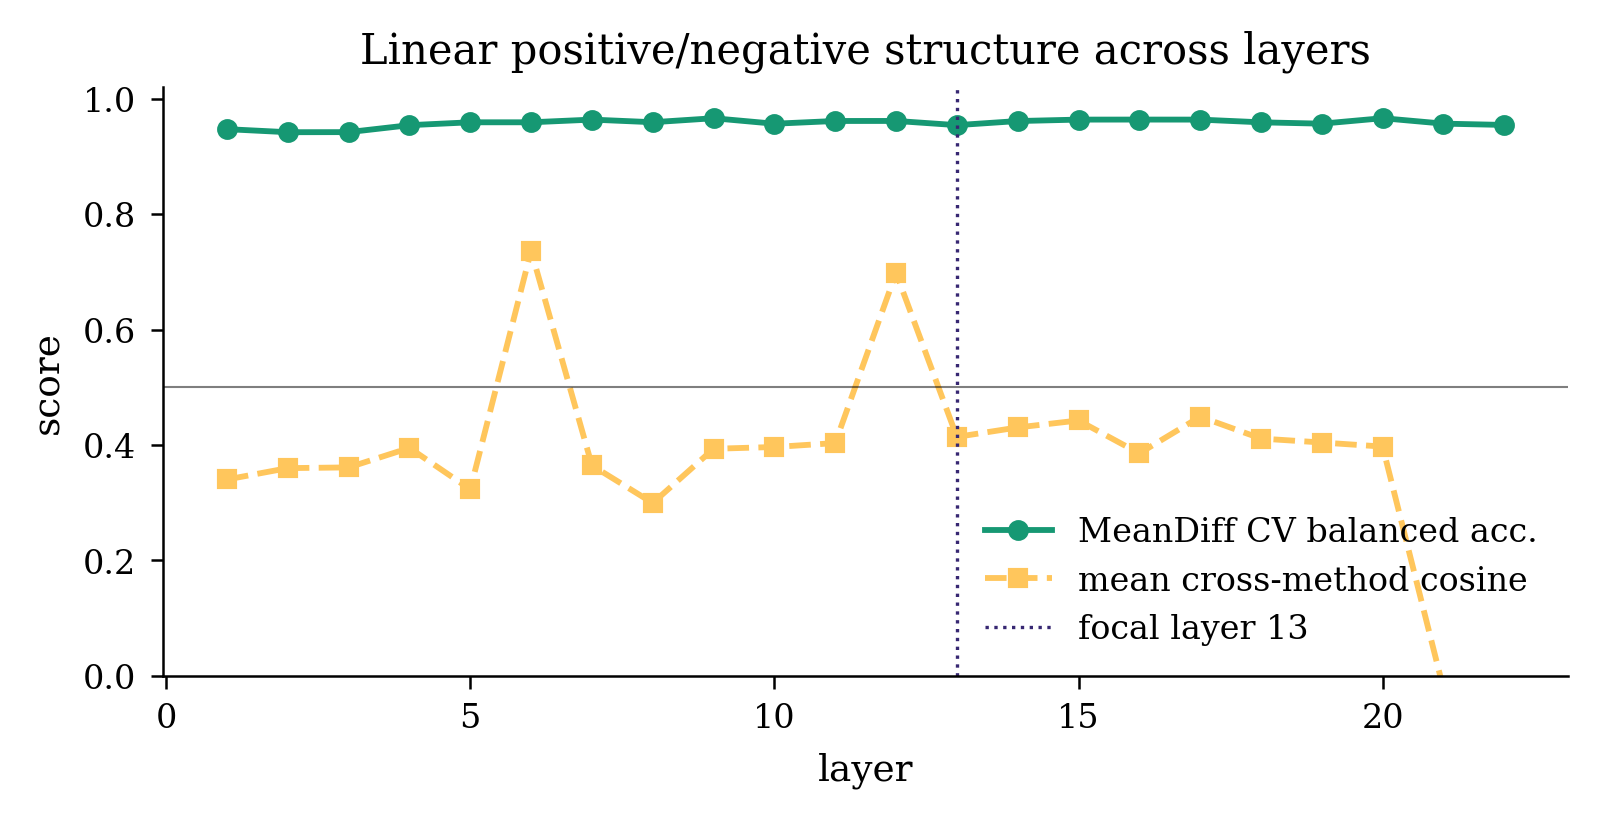
\includegraphics[width=0.49\textwidth]{replication_tigges/avg_token/layer_sweep.png}
\caption{Binary balanced accuracy across layers. \emph{Left:} last token.
\emph{Right:} mean pooling. The axis is recoverable throughout the network, with
a broad plateau around the focal layer~$13$.}
\label{fig:cv-layer}
\end{figure}

\begin{figure}[t]
\centering

\includegraphics[width=0.32\textwidth]{replication_tigges/last_token/direction_agreement_neutral_vs_negative_raw.png}

\includegraphics[width=0.32\textwidth]{replication_tigges/last_token/direction_agreement_positive_vs_neutral_raw.png}

\includegraphics[width=0.32\textwidth]{replication_tigges/last_token/direction_agreement_positive_vs_negative_raw.png}

\includegraphics[width=0.32\textwidth]{replication_tigges/last_token/direction_agreement_neutral_vs_negative_centered.png}

\includegraphics[width=0.32\textwidth]{replication_tigges/last_token/direction_agreement_positive_vs_neutral_centered.png}

\includegraphics[width=0.32\textwidth]{replication_tigges/last_token/direction_agreement_positive_vs_negative_centered.png}
\caption{Direction agreement (last token), columns neu-vs-neg, pos-vs-neu,
pos-vs-neg. \emph{Top:} raw. \emph{Bottom:} within-scenario centered.}
\label{fig:dir-agree-last}
\end{figure}

\begin{figure}[t]
\centering
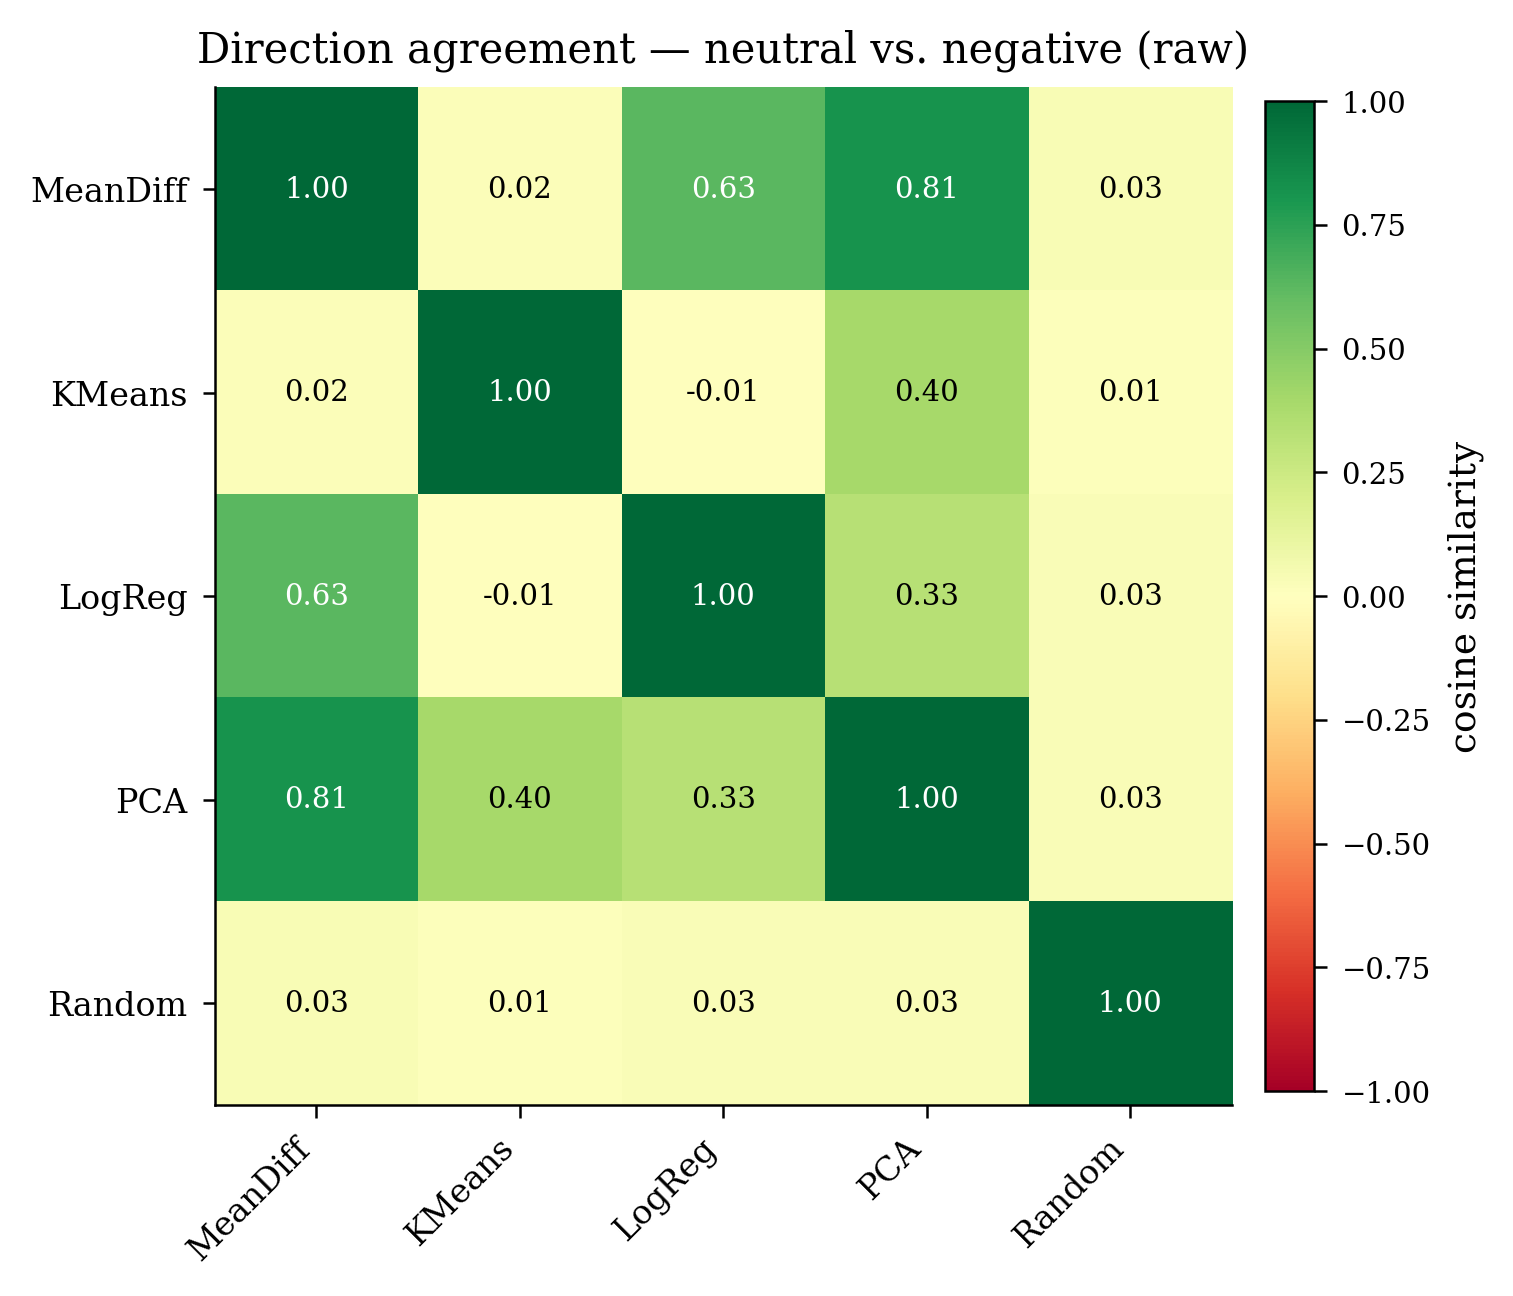
\includegraphics[width=0.32\textwidth]{replication_tigges/avg_token/direction_agreement_neutral_vs_negative_raw.png}
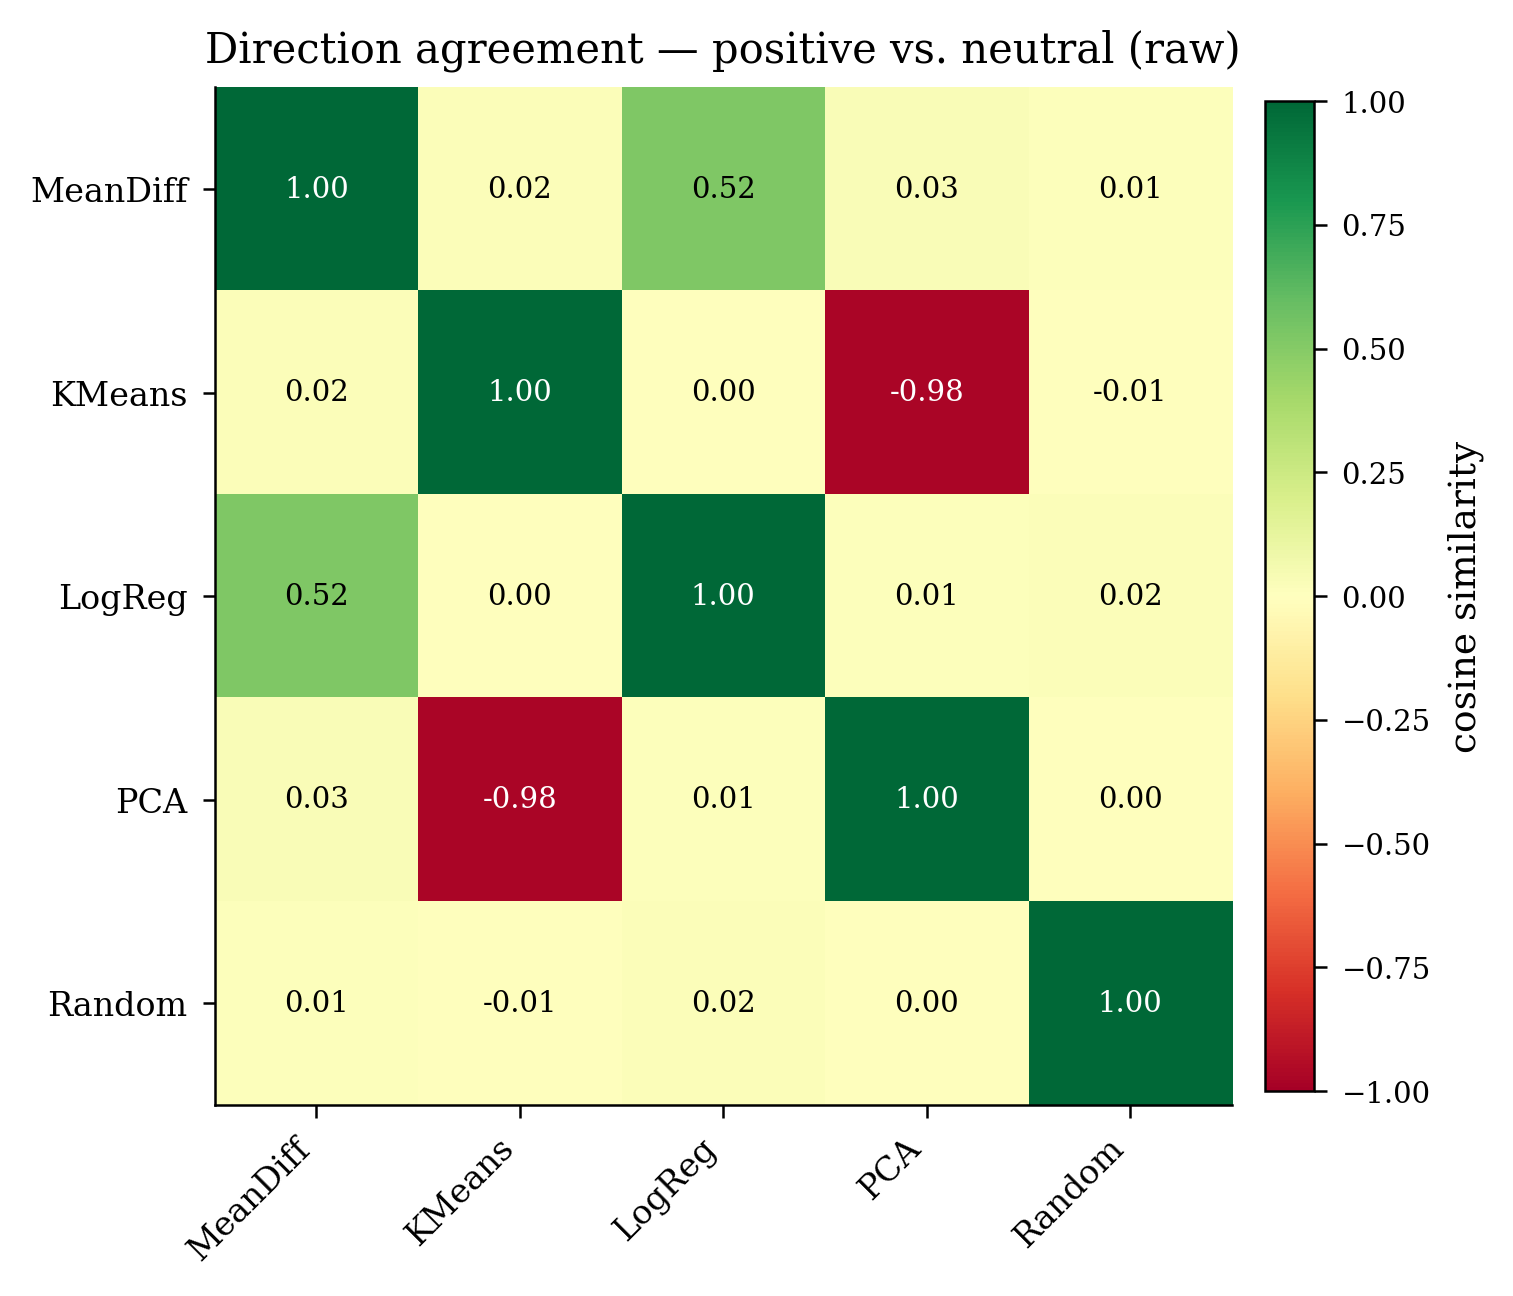
\includegraphics[width=0.32\textwidth]{replication_tigges/avg_token/direction_agreement_positive_vs_neutral_raw.png}
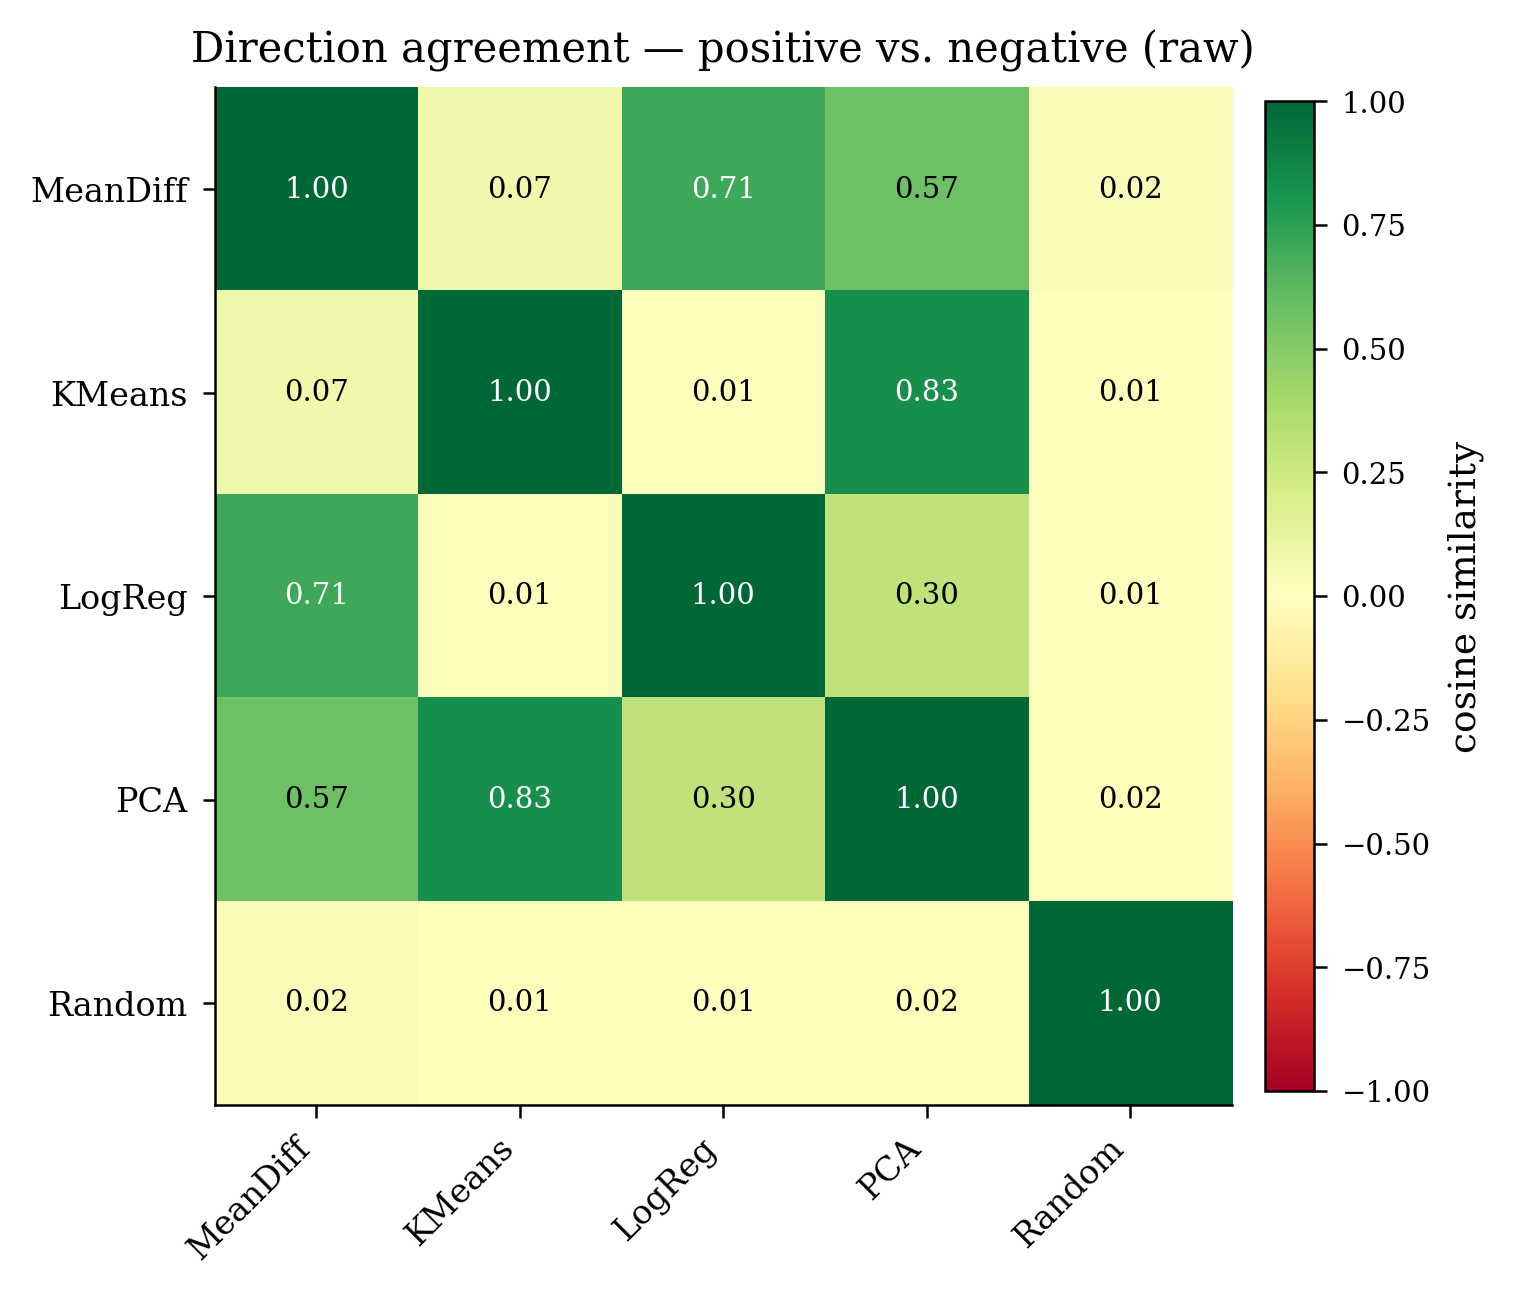
\includegraphics[width=0.32\textwidth]{replication_tigges/avg_token/direction_agreement_positive_vs_negative_raw.png}
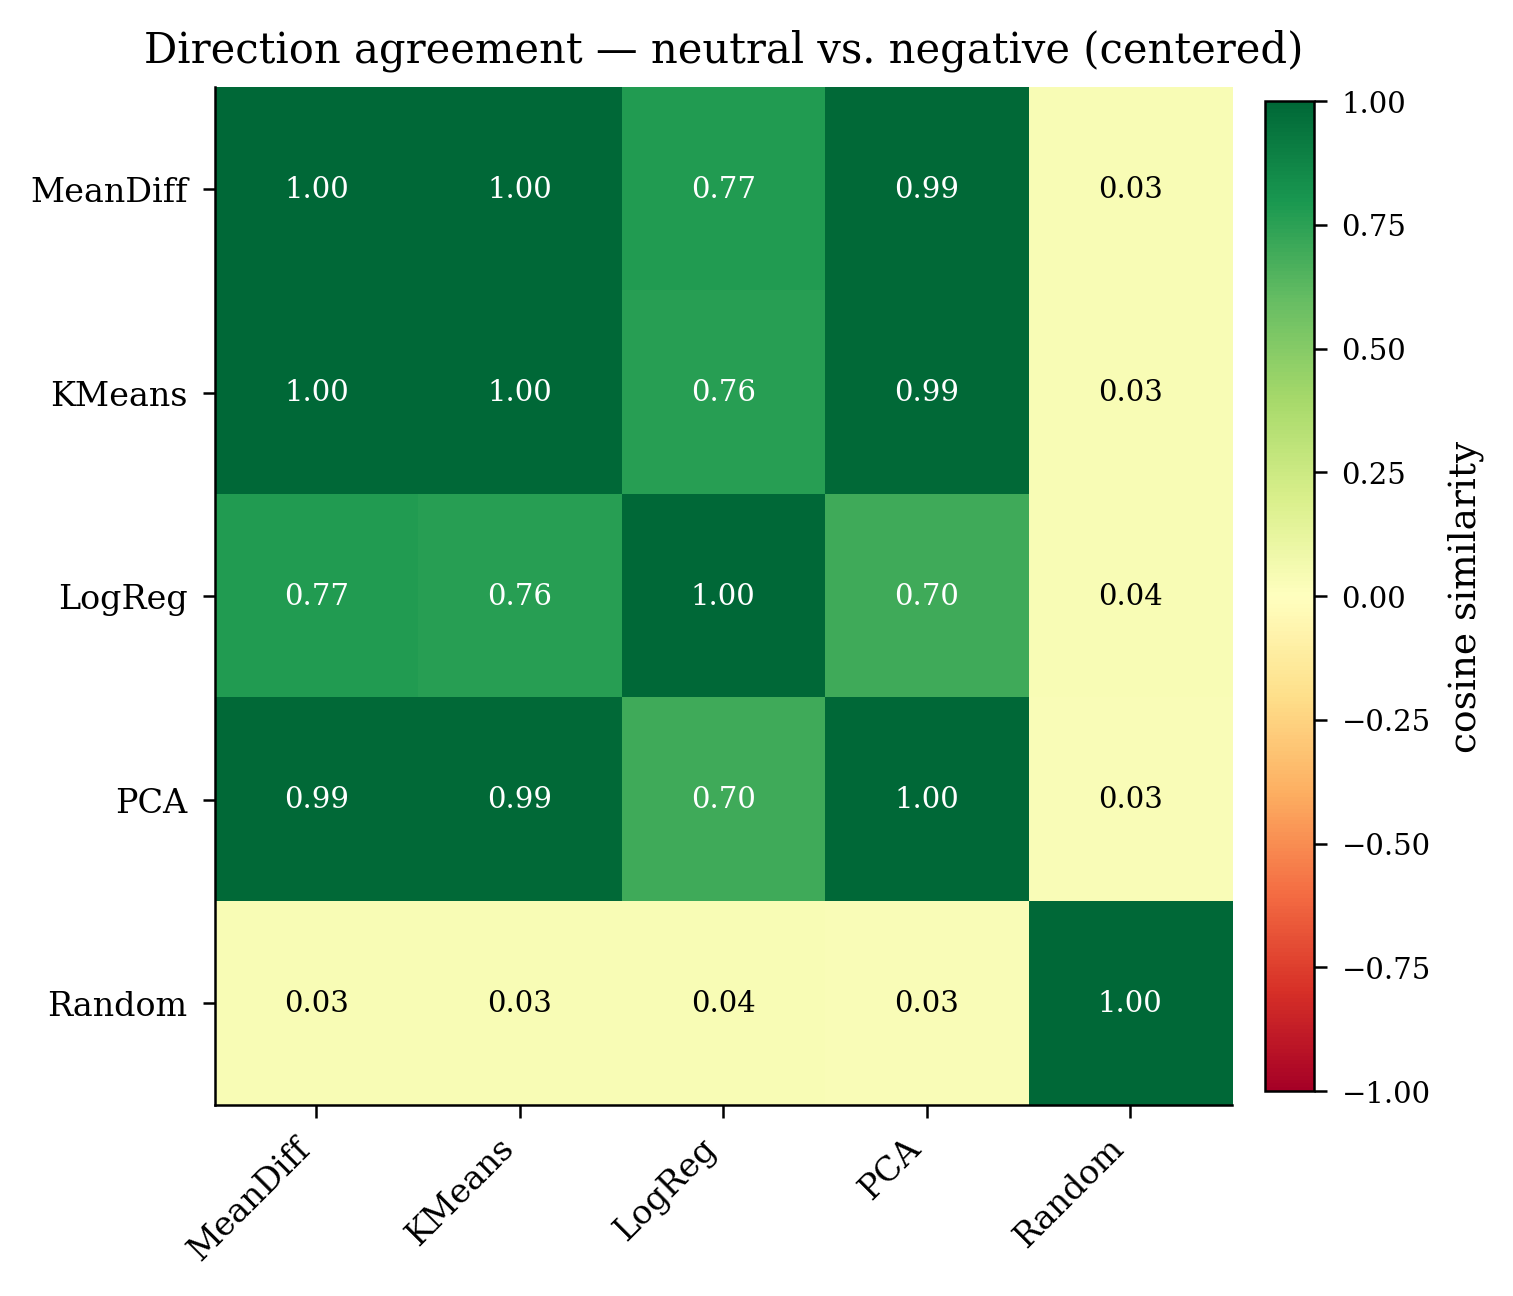
\includegraphics[width=0.32\textwidth]{replication_tigges/avg_token/direction_agreement_neutral_vs_negative_centered.png}
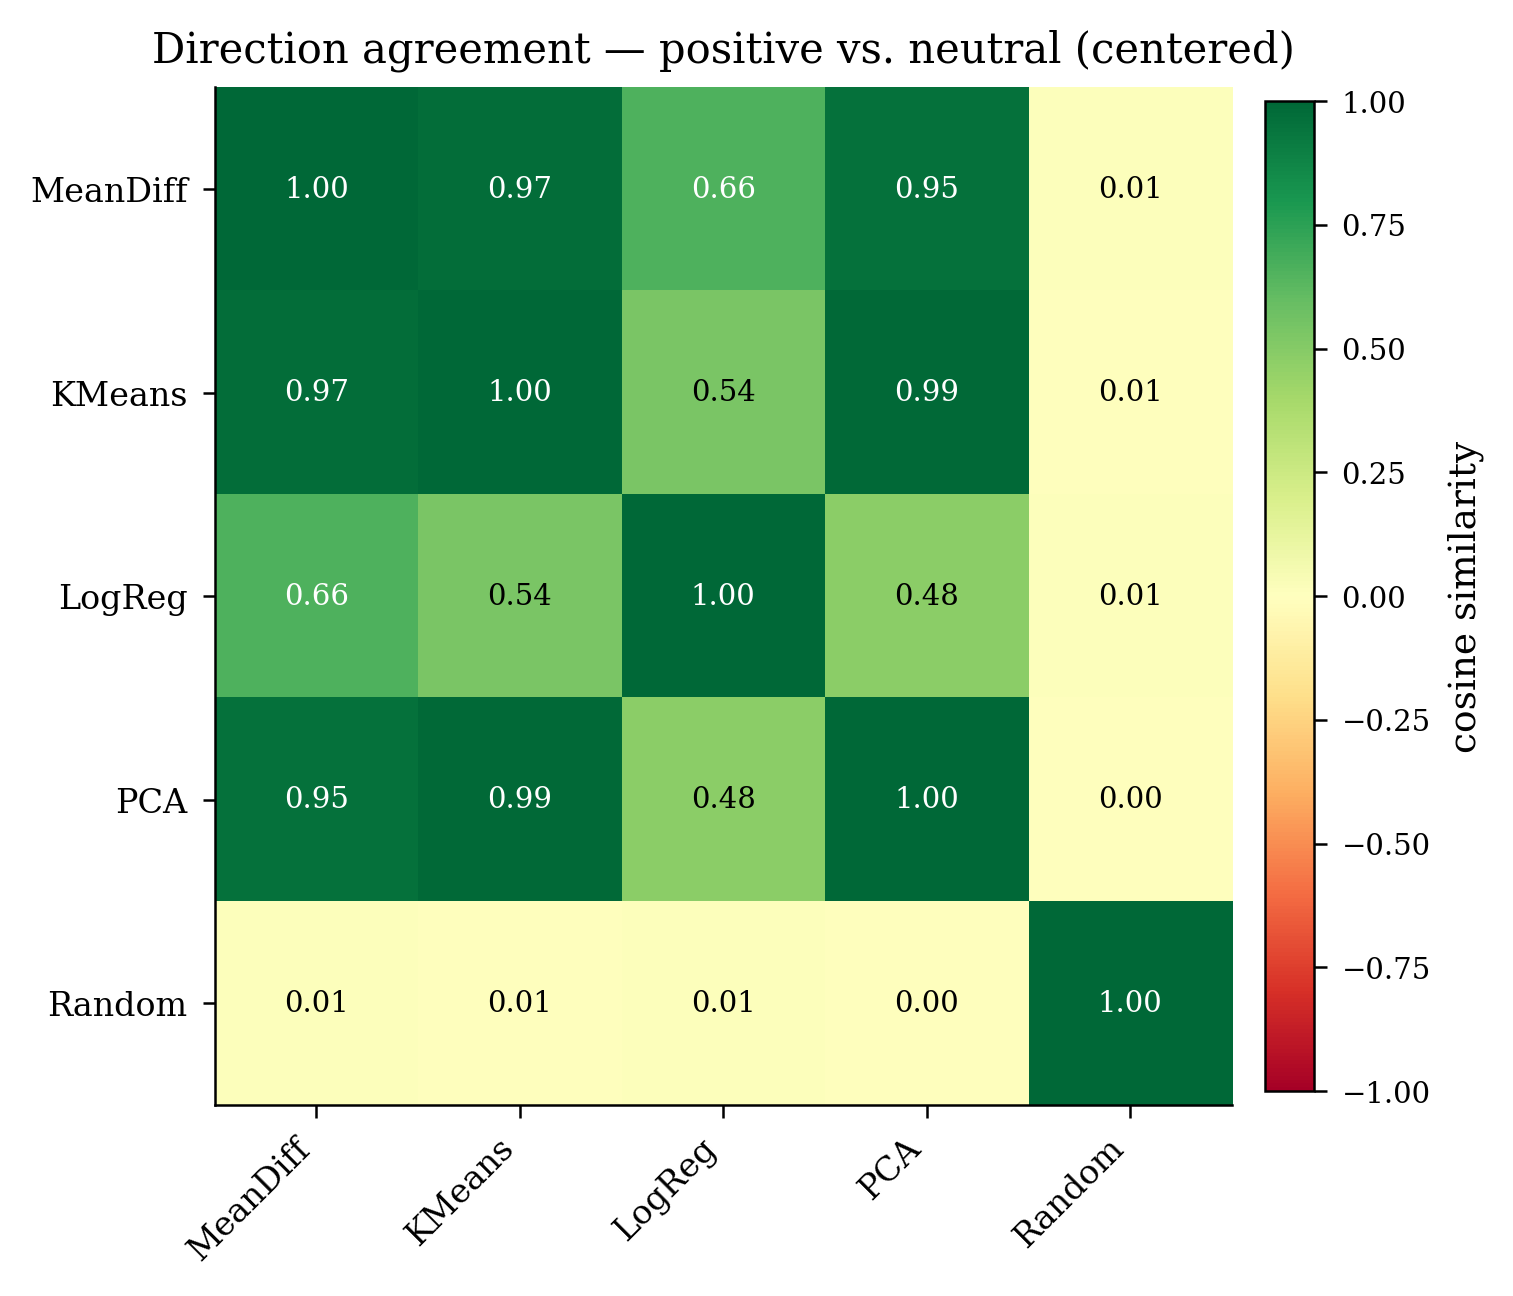
\includegraphics[width=0.32\textwidth]{replication_tigges/avg_token/direction_agreement_positive_vs_neutral_centered.png}
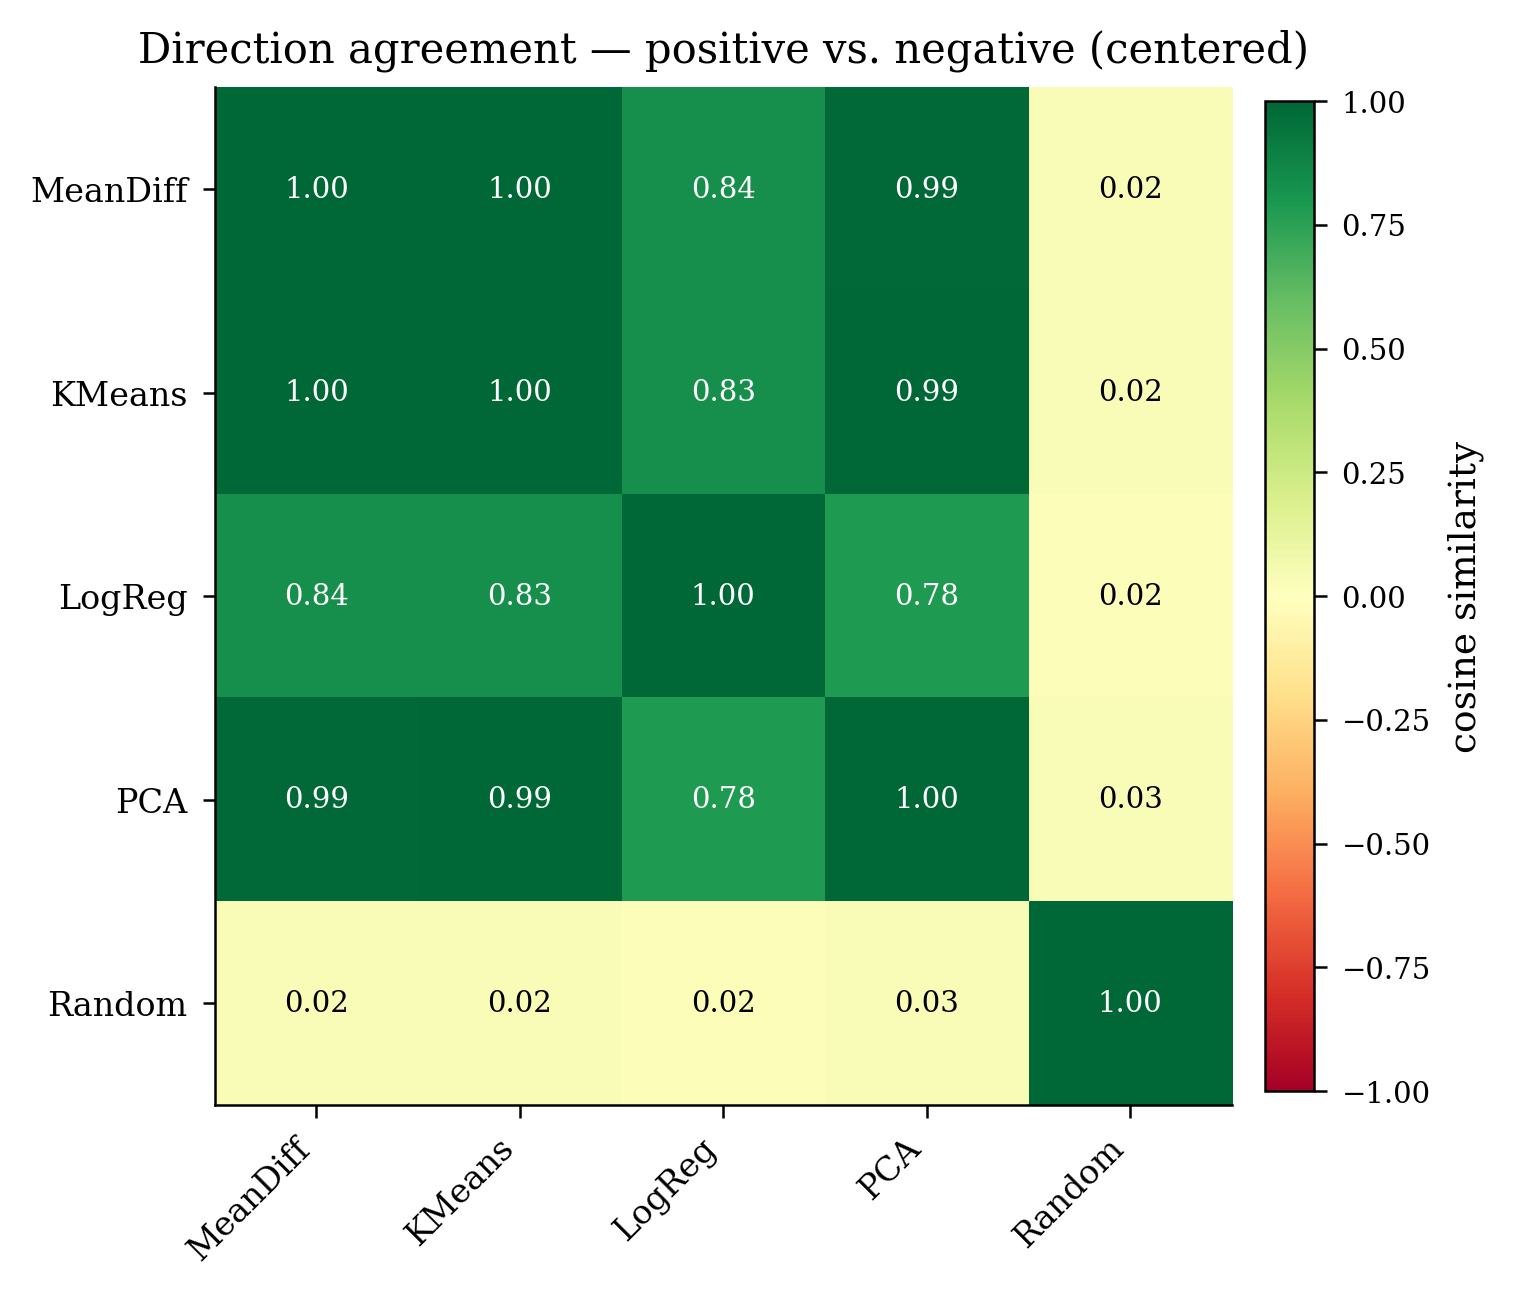
\includegraphics[width=0.32\textwidth]{replication_tigges/avg_token/direction_agreement_positive_vs_negative_centered.png}
\caption{Direction agreement (mean pooling), same layout as
\Cref{fig:dir-agree-last}.}
\label{fig:dir-agree-avg}
\end{figure}

\begin{figure}[t]
\centering

\includegraphics[width=0.32\textwidth]{replication_tigges/last_token/projection_neutral_vs_negative_raw.png}

\includegraphics[width=0.32\textwidth]{replication_tigges/last_token/projection_positive_vs_neutral_raw.png}

\includegraphics[width=0.32\textwidth]{replication_tigges/last_token/projection_positive_vs_negative_raw.png}

\includegraphics[width=0.32\textwidth]{replication_tigges/last_token/projection_neutral_vs_negative_centered.png}

\includegraphics[width=0.32\textwidth]{replication_tigges/last_token/projection_positive_vs_neutral_centered.png}

\includegraphics[width=0.32\textwidth]{replication_tigges/last_token/projection_positive_vs_negative_centered.png}
\caption{Projection onto the difference-of-means axis (last token), columns
neu-vs-neg, pos-vs-neu, pos-vs-neg. \emph{Top:} raw. \emph{Bottom:} centered.}
\label{fig:proj-last}
\end{figure}

\begin{figure}[t]
\centering
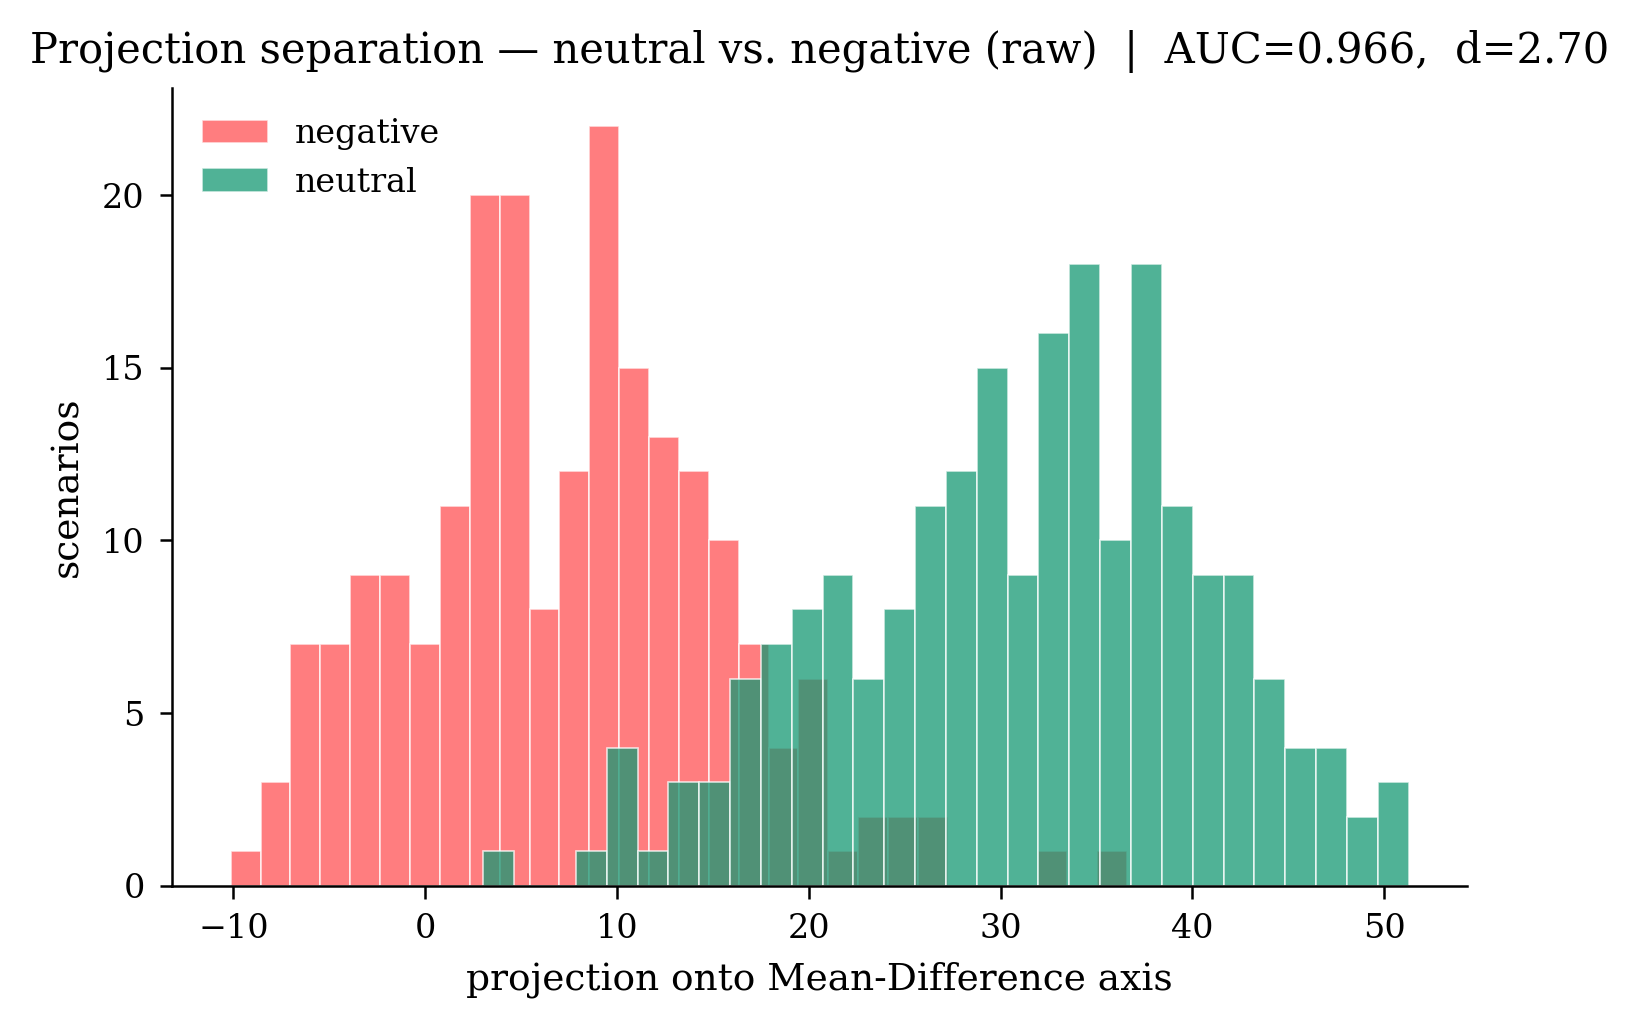
\includegraphics[width=0.32\textwidth]{replication_tigges/avg_token/projection_neutral_vs_negative_raw.png}
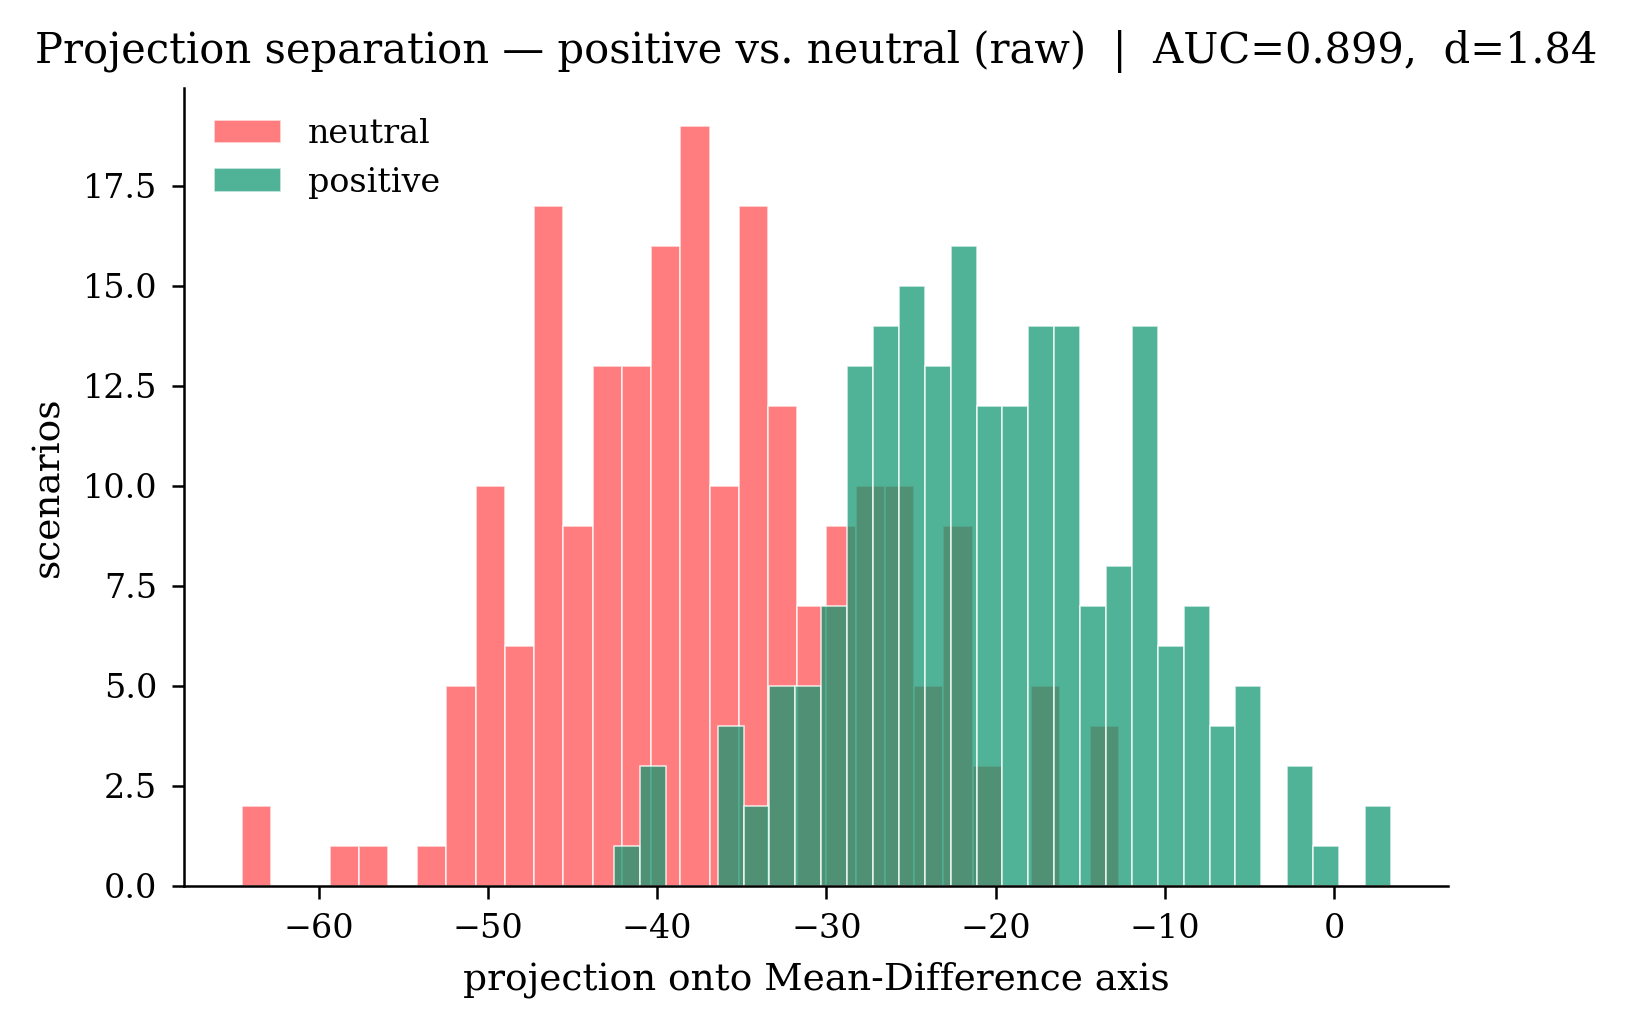
\includegraphics[width=0.32\textwidth]{replication_tigges/avg_token/projection_positive_vs_neutral_raw.png}
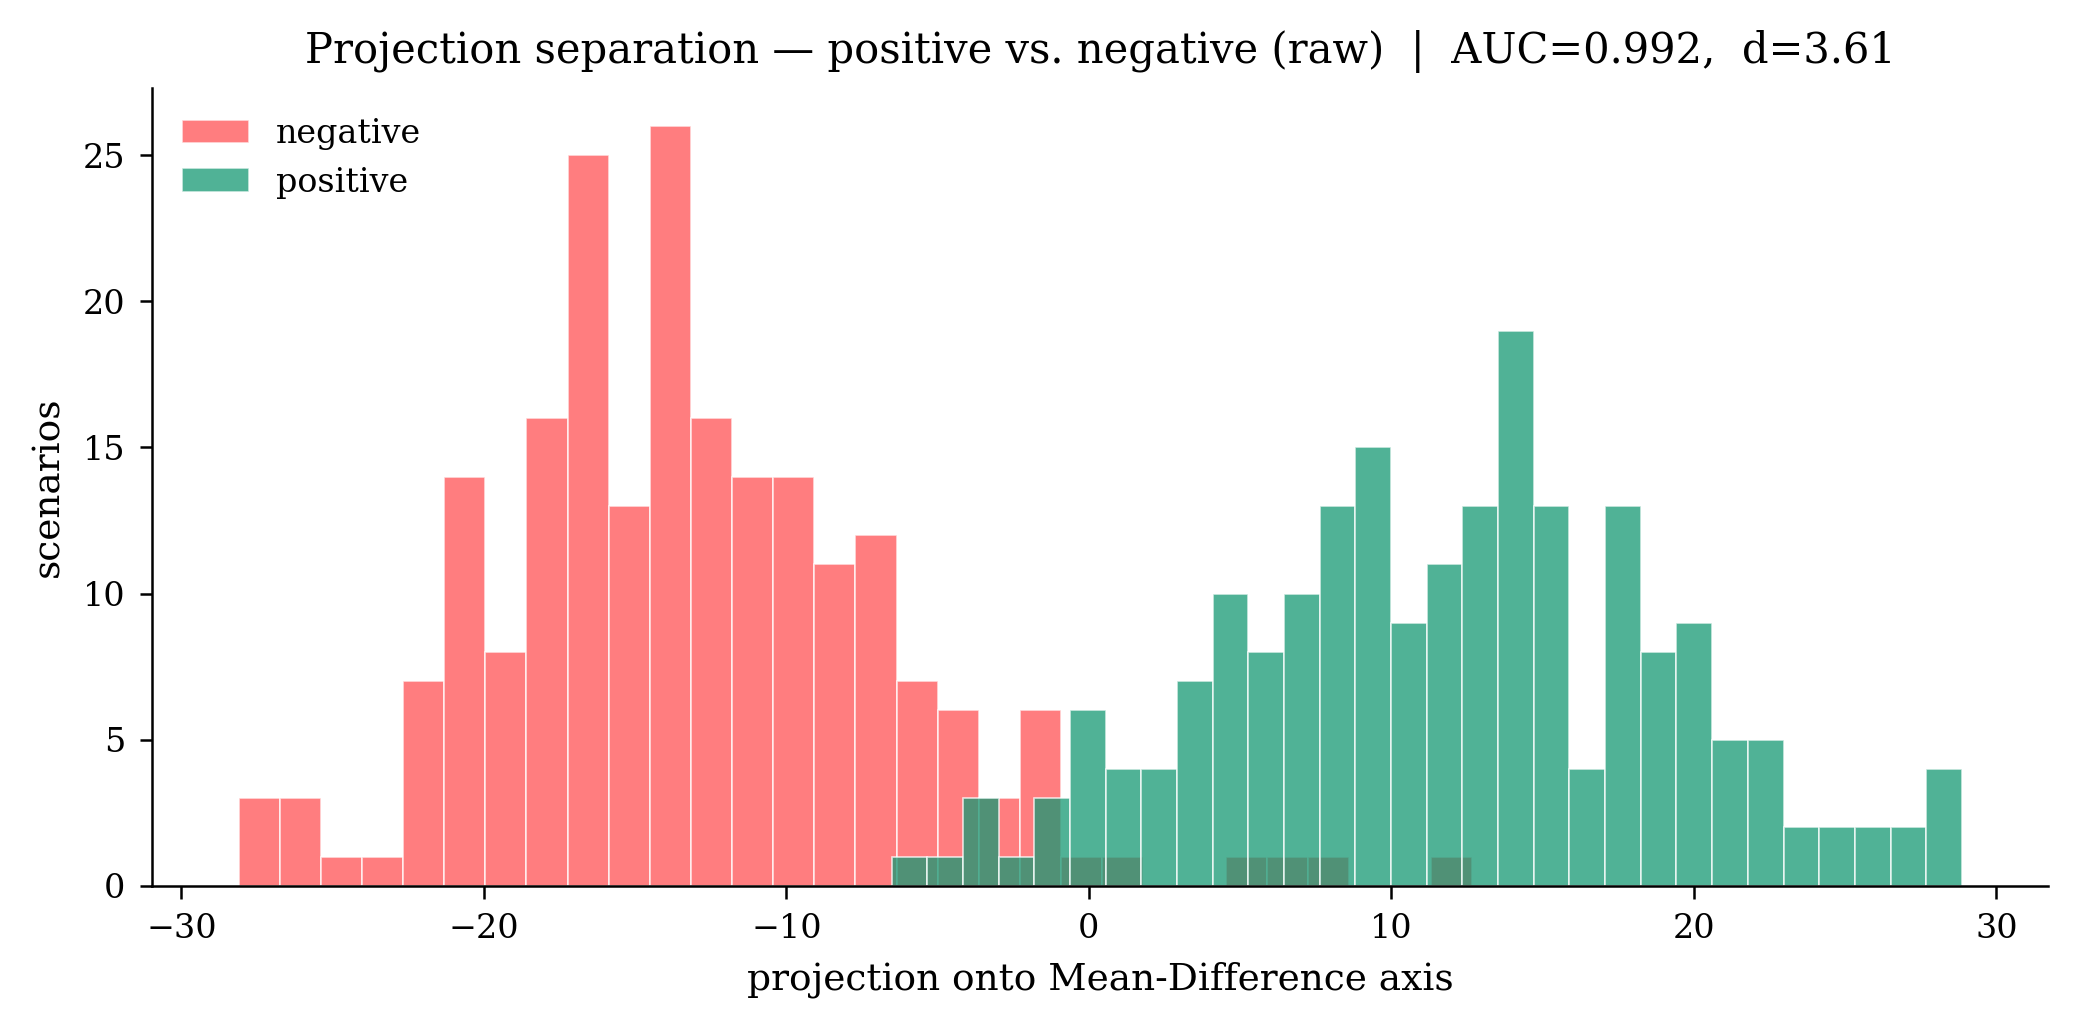
\includegraphics[width=0.32\textwidth]{replication_tigges/avg_token/projection_positive_vs_negative_raw.png}
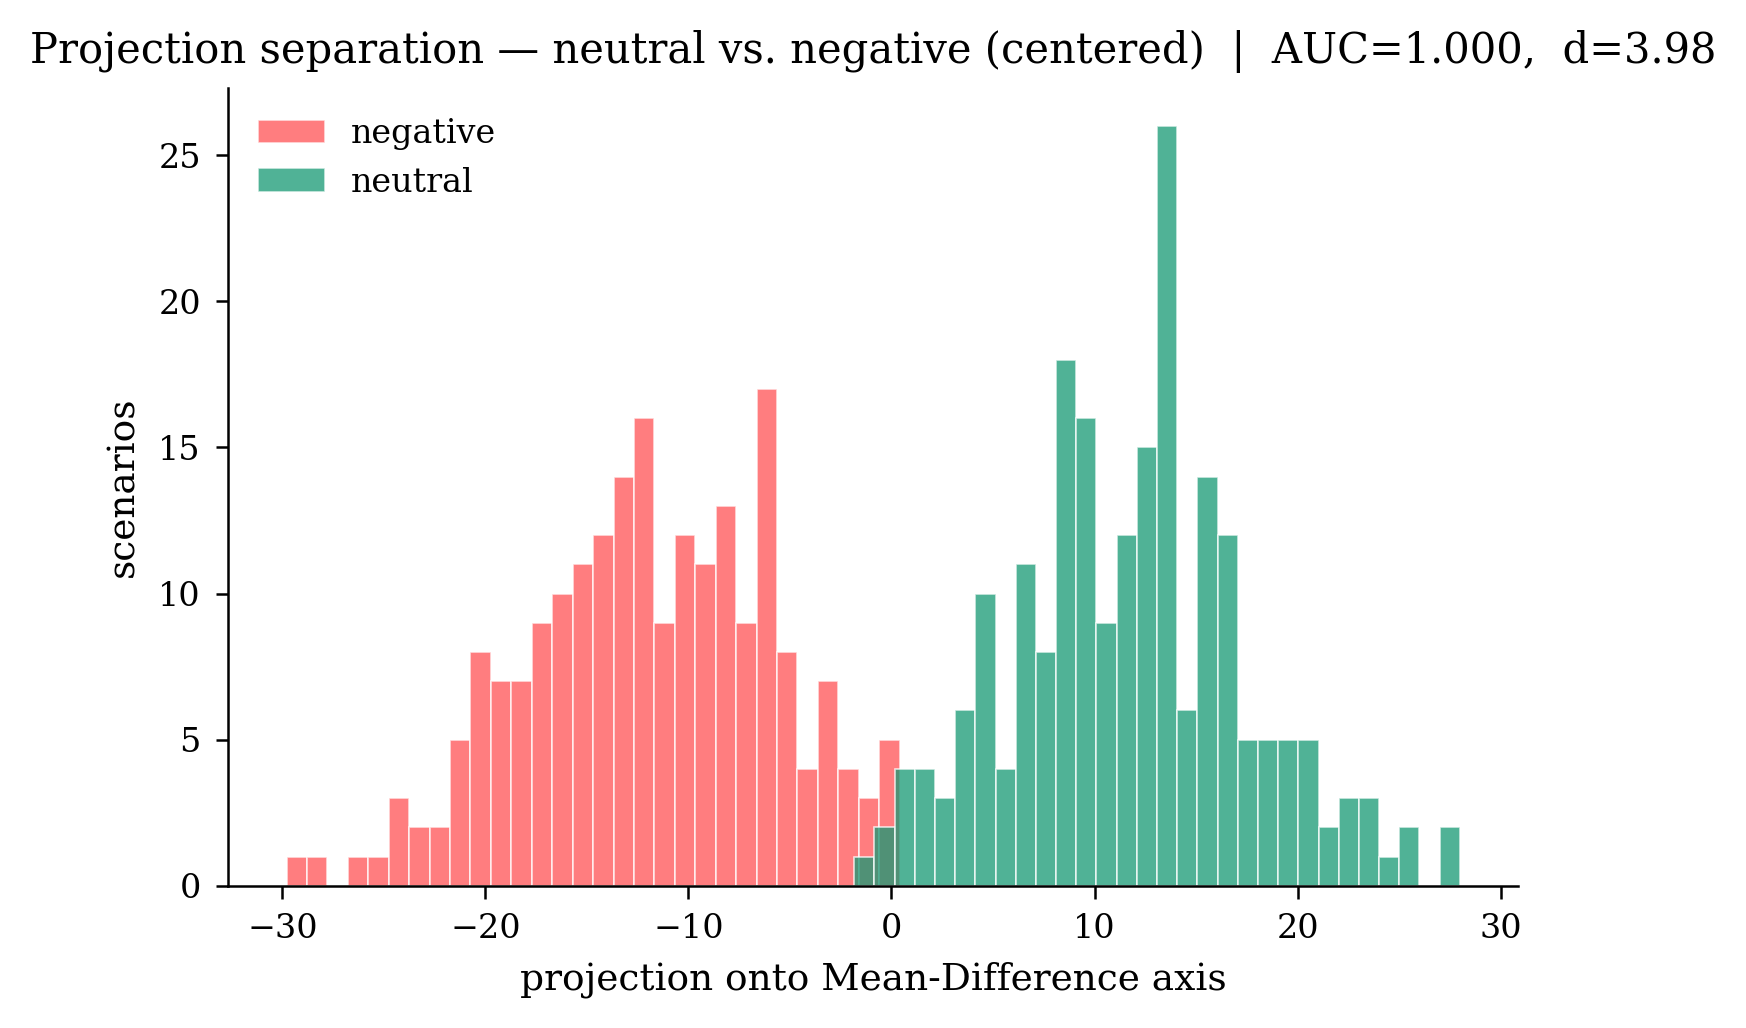
\includegraphics[width=0.32\textwidth]{replication_tigges/avg_token/projection_neutral_vs_negative_centered.png}
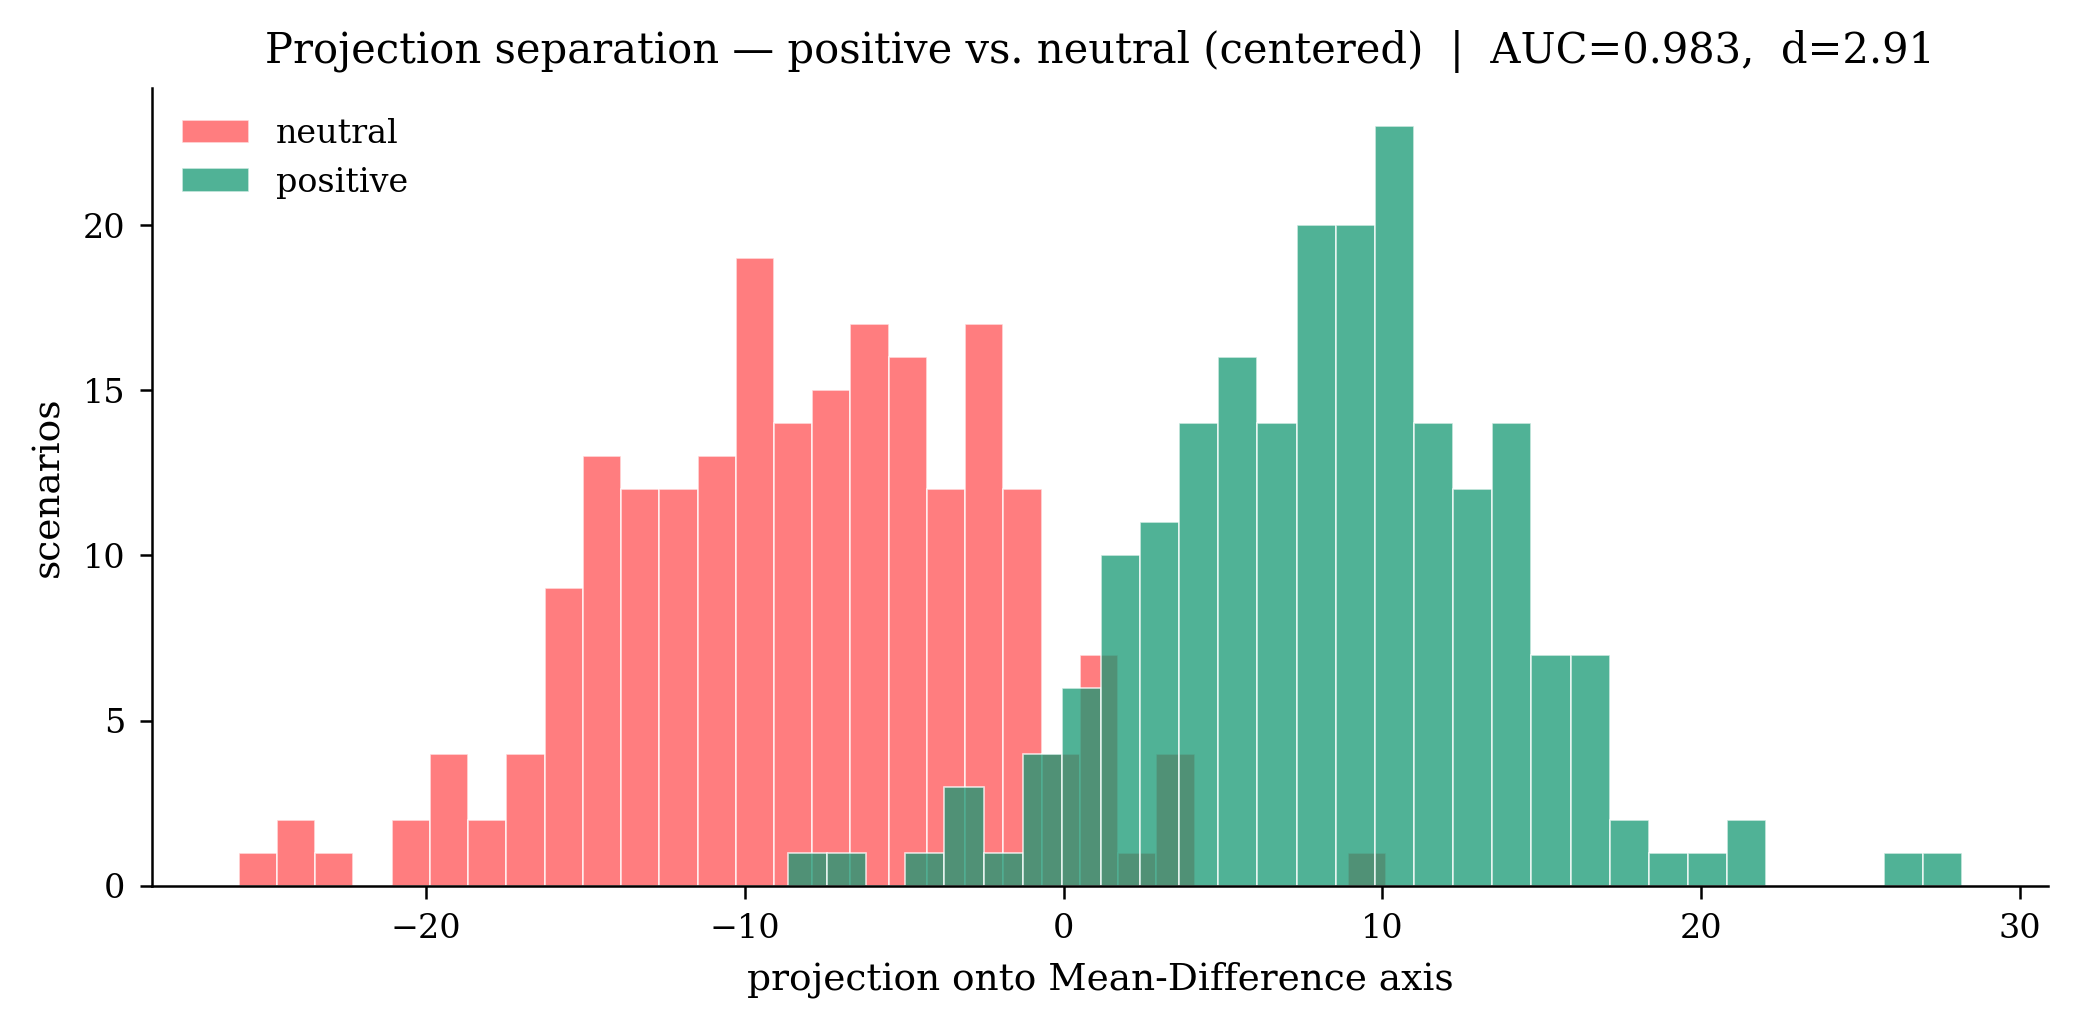
\includegraphics[width=0.32\textwidth]{replication_tigges/avg_token/projection_positive_vs_neutral_centered.png}
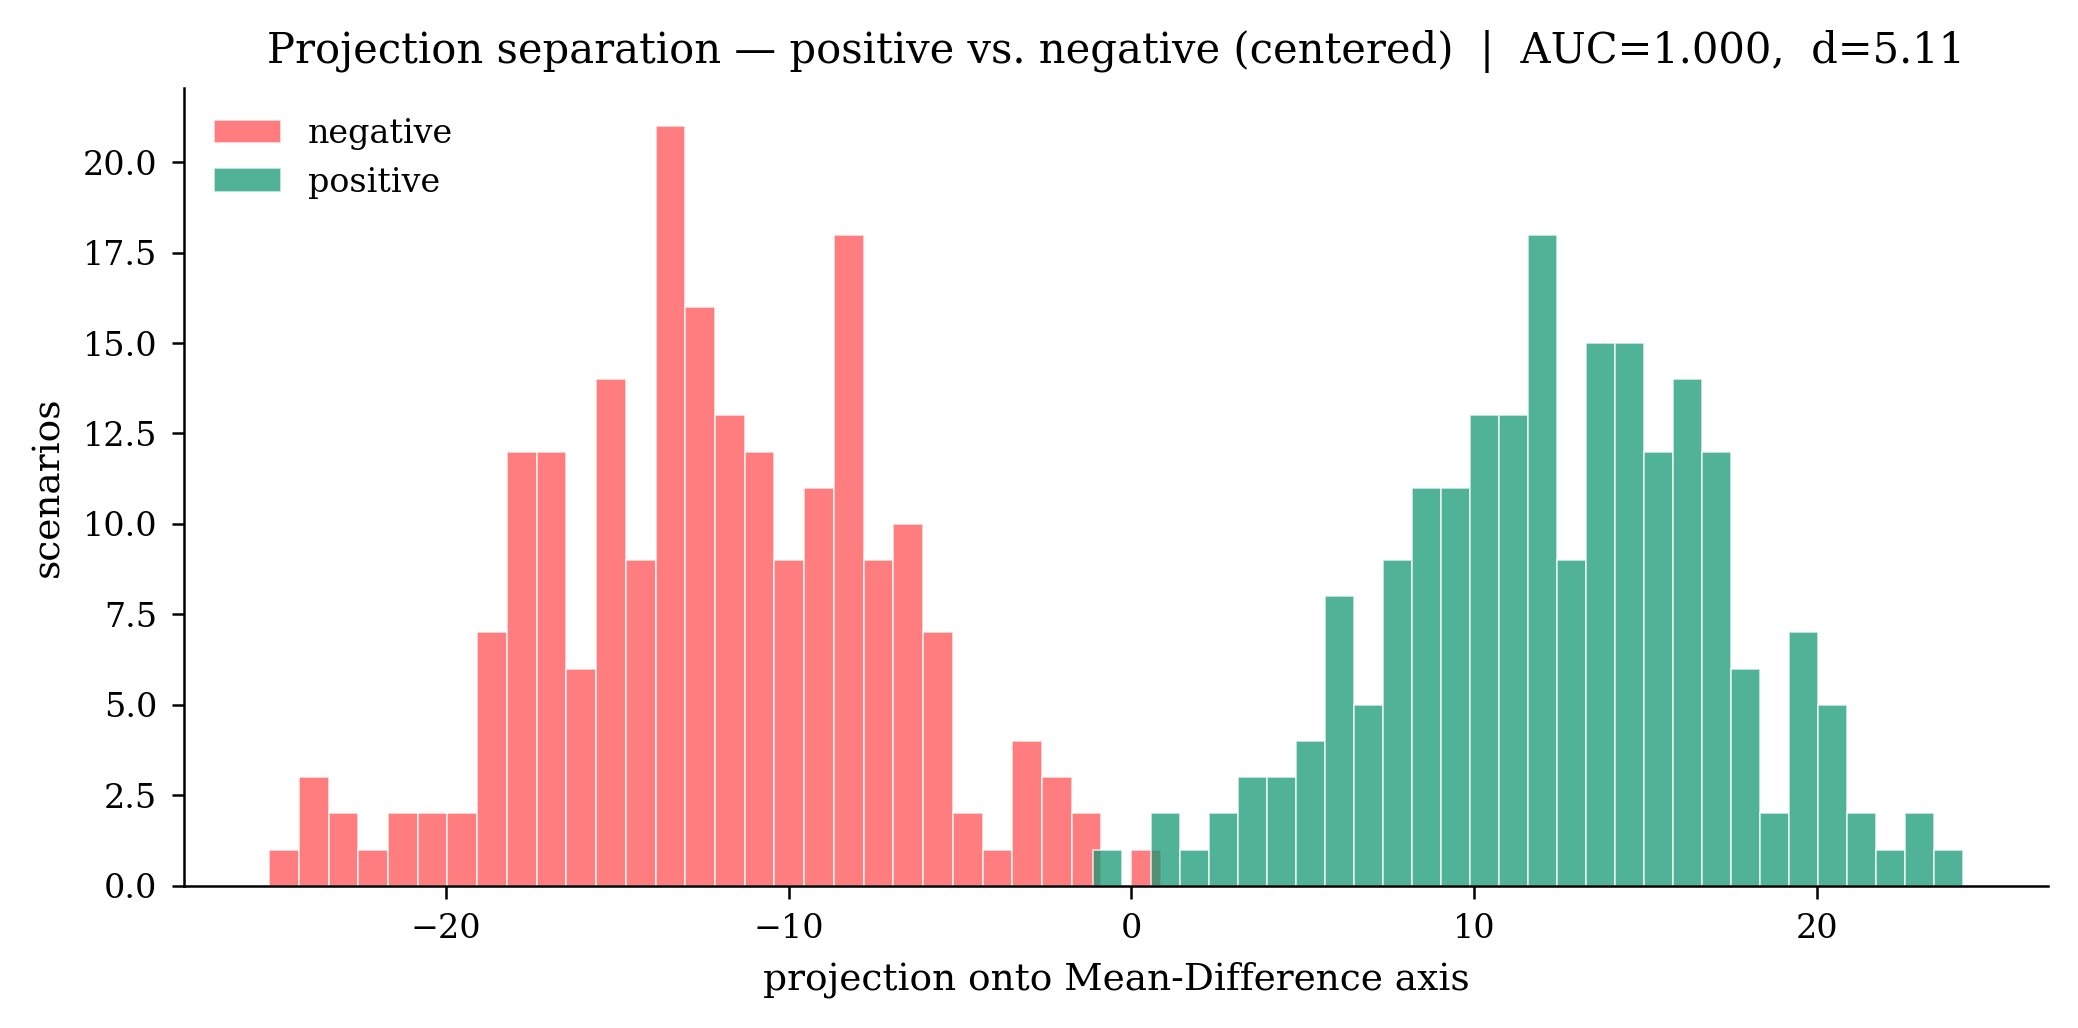
\includegraphics[width=0.32\textwidth]{replication_tigges/avg_token/projection_positive_vs_negative_centered.png}
\caption{Projection onto the difference-of-means axis (mean pooling), same layout
as \Cref{fig:proj-last}.}
\label{fig:proj-avg}
\end{figure}

\clearpage
\subsection{Graded-ladder geometry}\label{app:res-geometry}

\Cref{tab:geom-both} reports the seven geometry descriptors with
scenario-bootstrap $95\%$ intervals for both poolings, and \Cref{tab:noise-both}
the linear-ladder noise null. The bend is unambiguous in both: the adjacent steps
anti-align (step cosine $-0.23$/$-0.29$), the apex sits near a right angle rather
than the straight-ladder $180^\circ$, and the midpoint residual is far above what
noise on a straight ladder can produce ($p=0.001$). \Cref{tab:per-intent} breaks
the geometry down by communicative intent: every one of the ten intents is bent
(apex $59$--$90^\circ$, none near $180^\circ$), with requests and disagreements
the straightest and complaints, corrections, and refusals the most bent under
both poolings. Figures \ref{fig:geometry} and \ref{fig:geometry-avg} show the
bootstrap and noise-null distributions; \Cref{fig:per-intent} shows the
per-intent triangles.

\begin{table}[t]
\centering
\small
\begin{tabular}{lrr}
\toprule
 & Last token & Mean pooling \\
Descriptor & point\,[$95\%$\,CI] & point\,[$95\%$\,CI] \\
\midrule
Step cosine          & $-0.229$\,[$-0.331,-0.127$] & $-0.289$\,[$-0.376,-0.212$] \\
Apex angle ($^\circ$) & $76.8$\,[$70.7,82.7$] & $73.2$\,[$67.9,77.8$] \\
Midpoint residual    & $0.613$\,[$0.560,0.679$] & $0.661$\,[$0.612,0.723$] \\
Markedness           & $0.537$\,[$0.487,0.617$] & $0.619$\,[$0.571,0.686$] \\
Markedness ratio     & $1.073$\,[$0.974,1.233$] & $1.238$\,[$1.141,1.372$] \\
Valence offset       & $0.297$\,[$0.214,0.346$] & $0.232$\,[$0.159,0.294$] \\
Effective vertices   & $4.69$\,[$4.35,5.09$] & $4.92$\,[$4.63,5.30$] \\
\bottomrule
\end{tabular}
\caption{Pooled triple-geometry descriptors with scenario-bootstrap intervals
($1000$ resamples), layer~13. A straight ladder would give step cosine $+1$,
apex $180^\circ$, and midpoint residual $0$.}
\label{tab:geom-both}
\end{table}

\begin{table}[t]
\centering
\small
\begin{tabular}{lrrrrr}
\toprule
 & \multicolumn{2}{c}{observed} & \multicolumn{2}{c}{null mean (sd)} & \\
\cmidrule(lr){2-3}\cmidrule(lr){4-5}
Metric & last & avg & last & avg & $p$ \\
\midrule
Step cosine       & $-0.229$ & $-0.289$ & $0.919\,(0.015)$ & $0.946\,(0.010)$ & $0.001$ \\
Midpoint residual & $0.613$  & $0.661$  & $0.104\,(0.010)$ & $0.084\,(0.008)$ & $0.001$ \\
\bottomrule
\end{tabular}
\caption{Linear-ladder noise null ($N=1000$): Gaussian noise calibrated to the
observed scatter, placed on a perfectly straight ladder, cannot reproduce either
the negative step cosine or the large midpoint residual, under either pooling.}
\label{tab:noise-both}
\end{table}

\begin{table}[t]
\centering
\small
\setlength{\tabcolsep}{5pt}
\begin{tabular}{lrrrrrrr}
\toprule
 & & \multicolumn{3}{c}{Last token} & \multicolumn{3}{c}{Mean pooling} \\
\cmidrule(lr){3-5}\cmidrule(lr){6-8}
Intent & $n$ & Apex$^\circ$ & Step cos & Mid. & Apex$^\circ$ & Step cos & Mid. \\
\midrule
apology               & 8  & 78.2 & $-0.20$ & 0.60 & 84.0 & $-0.10$ & 0.55 \\
bad-news-delivery     & 4  & 72.3 & $-0.30$ & 0.64 & 59.3 & $-0.51$ & 0.83 \\
complaint             & 7  & 66.2 & $-0.40$ & 0.76 & 63.7 & $-0.44$ & 0.80 \\
correction            & 9  & 67.9 & $-0.38$ & 0.73 & 74.5 & $-0.27$ & 0.66 \\
criticism-or-feedback & 8  & 67.9 & $-0.38$ & 0.73 & 70.9 & $-0.33$ & 0.69 \\
disagreement          & 6  & 82.9 & $-0.12$ & 0.56 & 90.3 & $+0.01$ & 0.50 \\
inquiry-sensitive     & 4  & 79.8 & $-0.18$ & 0.60 & 74.6 & $-0.27$ & 0.66 \\
refusal               & 8  & 73.7 & $-0.28$ & 0.65 & 63.4 & $-0.45$ & 0.80 \\
reminder              & 6  & 73.2 & $-0.29$ & 0.66 & 71.2 & $-0.32$ & 0.68 \\
request               & 12 & 88.6 & $-0.02$ & 0.51 & 82.7 & $-0.13$ & 0.57 \\
\midrule
\textbf{ALL}          & 72 & 76.8 & $-0.23$ & 0.61 & 73.2 & $-0.29$ & 0.66 \\
\bottomrule
\end{tabular}
\caption{Triple geometry pooled within each communicative intent, both poolings
(layer~13). Apex angles stay well below the straight-ladder $180^\circ$ for every
intent.}
\label{tab:per-intent}
\end{table}

\begin{figure}[t]
\centering

\includegraphics[width=0.49\textwidth]{trait_geometry/last_token/geometry_bootstrap.png}

\includegraphics[width=0.49\textwidth]{trait_geometry/last_token/noise_null.png}
\caption{Triple geometry, last token. \emph{Left:} bootstrap distributions of the
geometry descriptors against the straight-ladder and pentagon references.
\emph{Right:} the linear-ladder noise null.}
\label{fig:geometry}
\end{figure}

\begin{figure}[t]
\centering
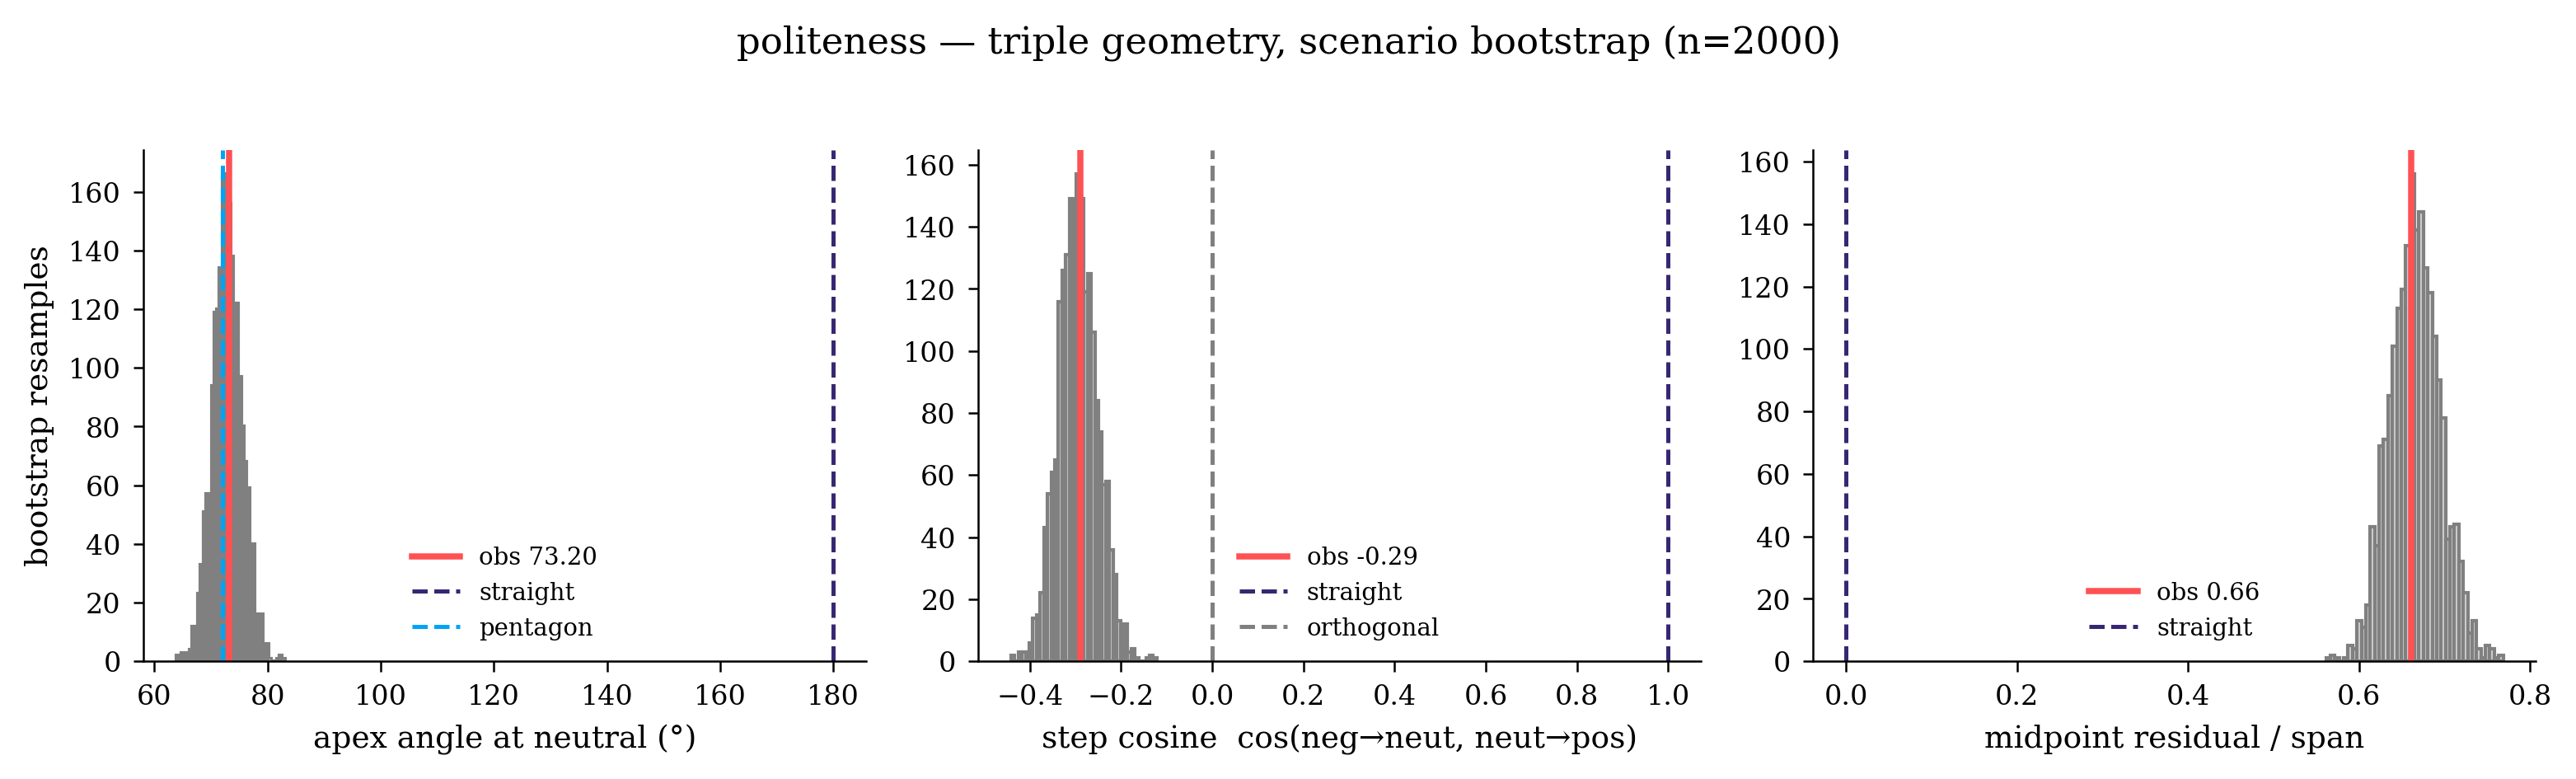
\includegraphics[width=0.49\textwidth]{trait_geometry/avg_token/geometry_bootstrap.png}
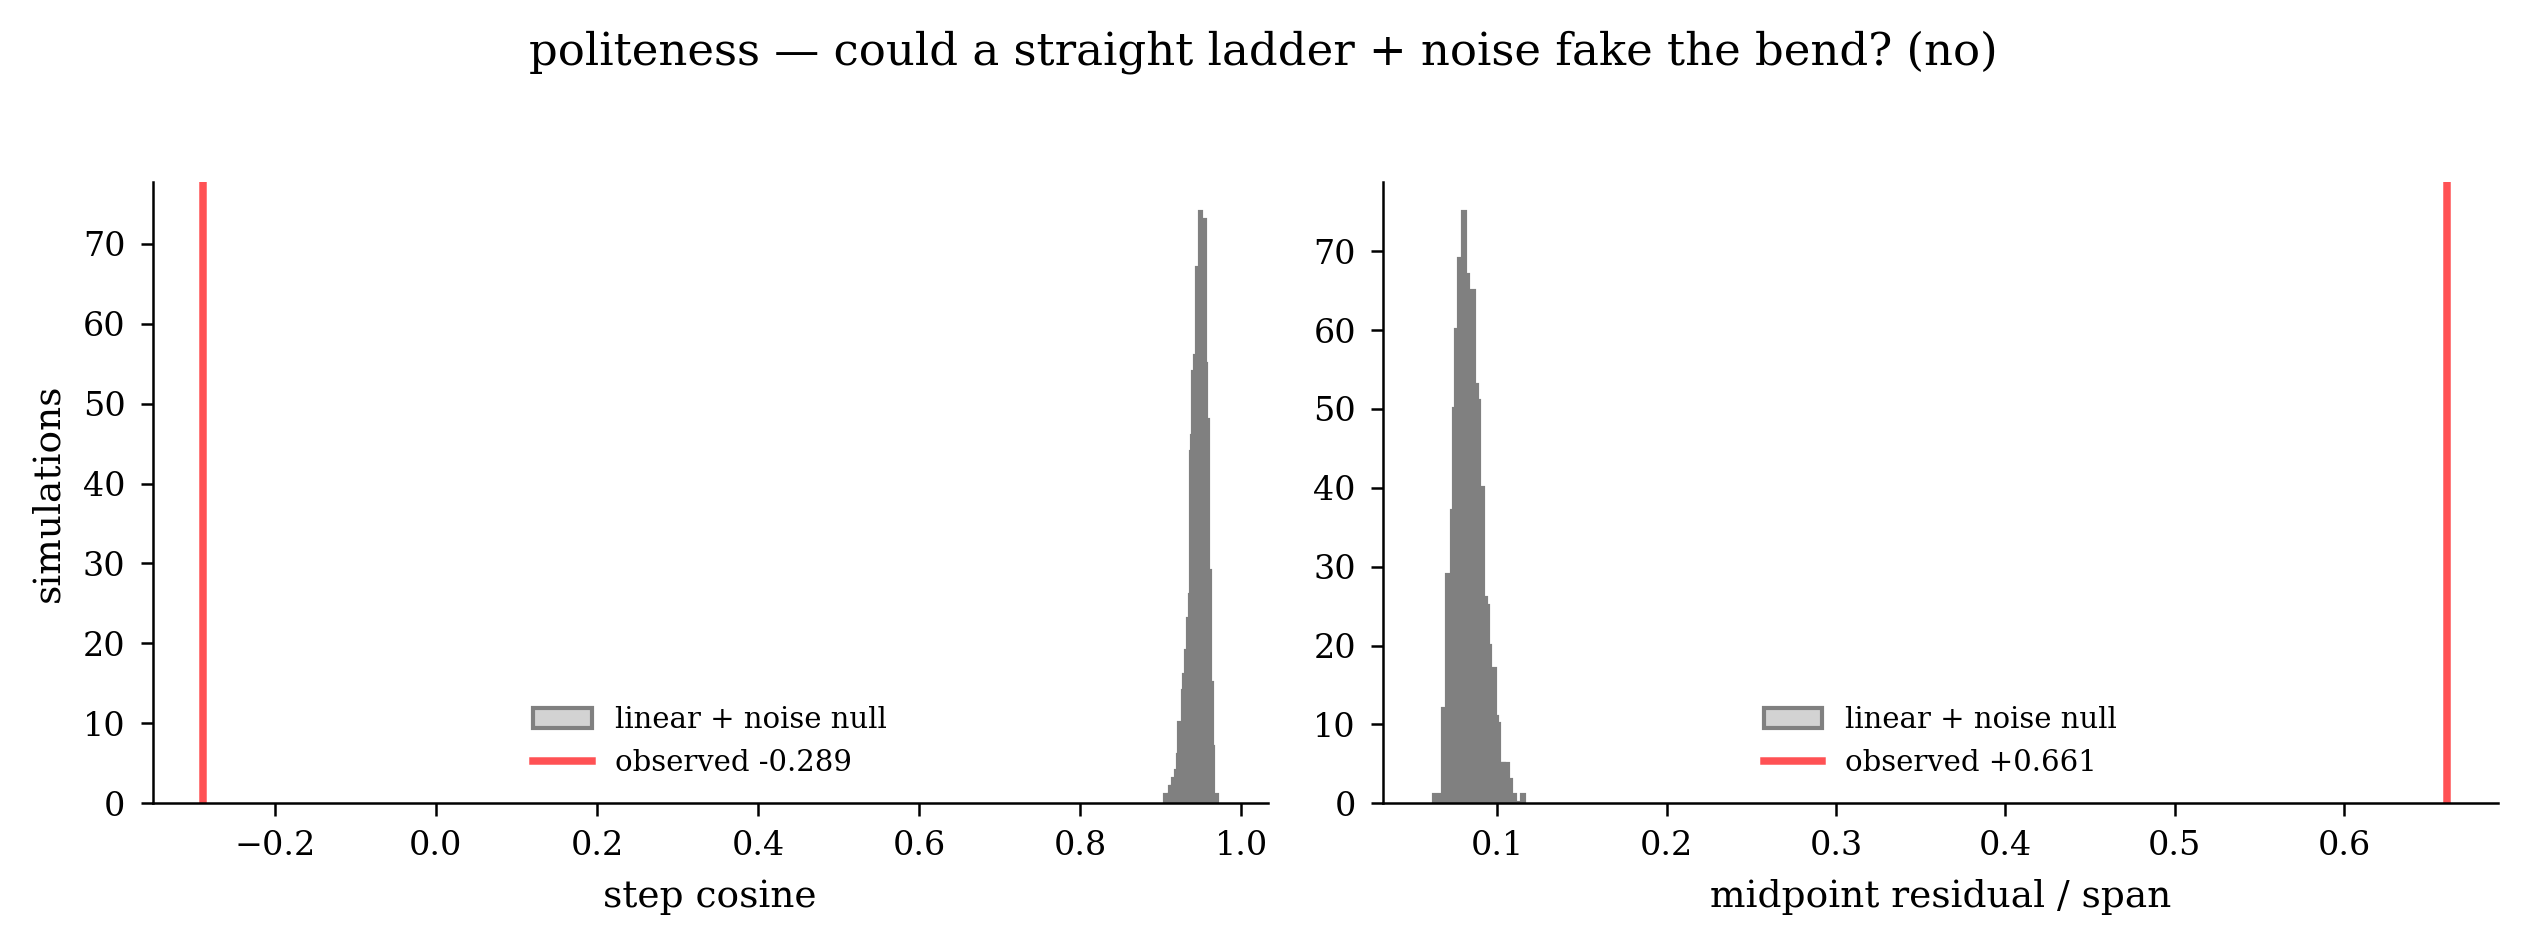
\includegraphics[width=0.49\textwidth]{trait_geometry/avg_token/noise_null.png}
\caption{Triple geometry, mean pooling; same panels as \Cref{fig:geometry}.}
\label{fig:geometry-avg}
\end{figure}

\begin{figure}[t]
\centering

\includegraphics[width=0.49\textwidth]{trait_geometry/last_token/per_intent_geometry.png}
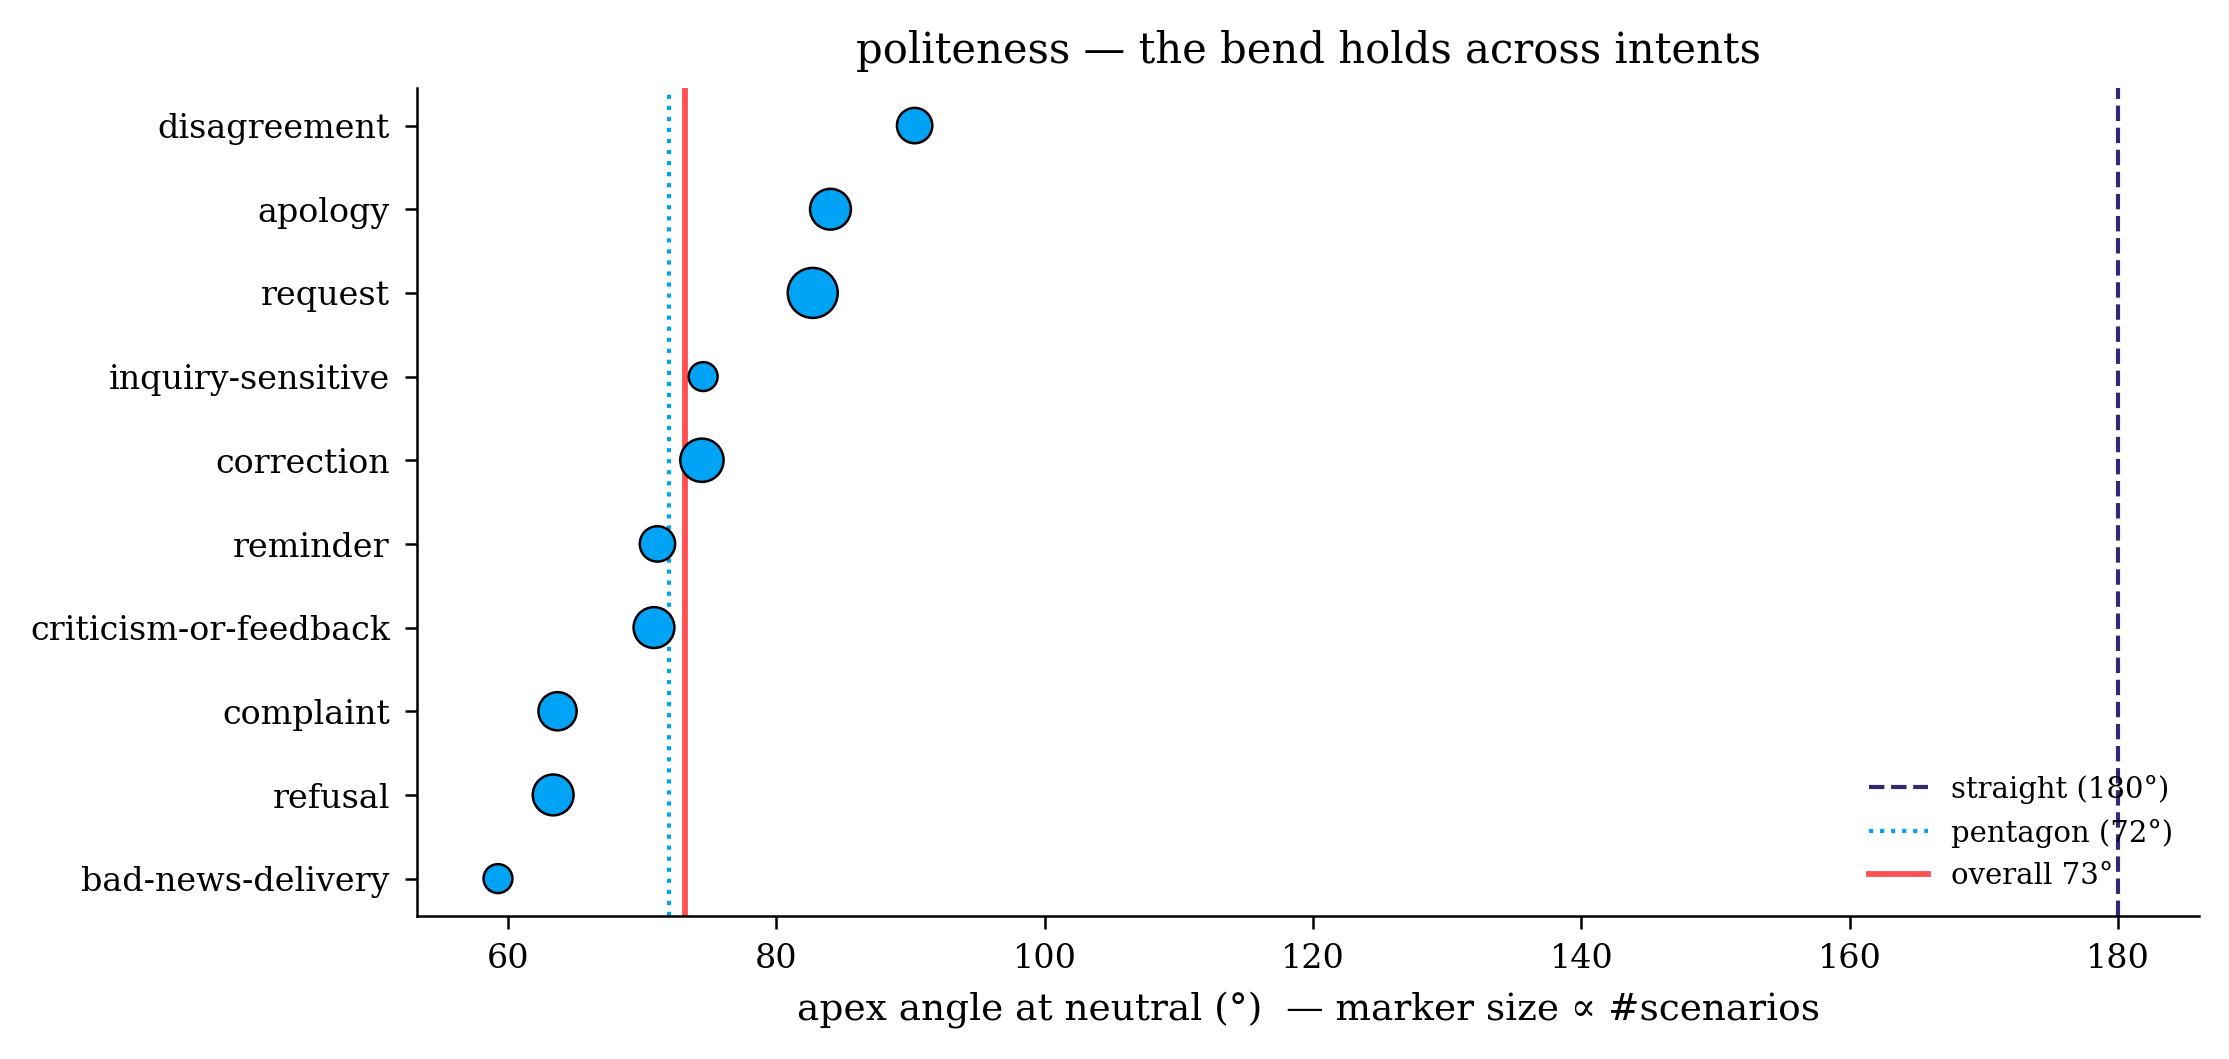
\includegraphics[width=0.49\textwidth]{trait_geometry/avg_token/per_intent_geometry.png}
\caption{Per-intent triangles. \emph{Left:} last token. \emph{Right:} mean
pooling. Every intent's triple is bent at an interior apex.}
\label{fig:per-intent}
\end{figure}

\clearpage
\subsection{Ordinal structure and the bend}\label{app:res-ordinal}

\Cref{tab:lin-both} reports the five ordinal-linearity metrics under the blocked
(within-scenario) and naive-pooled estimators for both poolings; blocking raises
every metric, and the within-scenario ladder is strongly ordered
($\rho=0.84$/$0.90$, probe $R^2=0.85$/$0.92$) yet its midpoint residual stays
high. \Cref{tab:perm-both} gives the within-scenario permutation null: all six
metrics clear it at $p\approx0.01$ (the sole exception is the mean-pooled
PC1-fraction at $p=0.05$, since the centroids are already nearly planar).
\Cref{tab:inner-both} re-measures the adjacent-step cosine under five inner
products, raw and disattenuated by split-half reliability; it remains negative in
every space under both poolings, so the bend is neither a coordinate nor a
reliability artefact. \Cref{tab:stepmat} lists the full step-vector cosine
matrix. The supporting figures are
\Cref{fig:ordinal,fig:ordinal-avg,fig:inner,fig:pca-last,fig:pca-avg,fig:lin-sweep}.

\begin{table}[t]
\centering
\small
\begin{tabular}{lrrrr}
\toprule
 & \multicolumn{2}{c}{Last token} & \multicolumn{2}{c}{Mean pooling} \\
\cmidrule(lr){2-3}\cmidrule(lr){4-5}
Metric & pooled & within & pooled & within \\
\midrule
Spearman $\rho$    & 0.775 & 0.841 & 0.812 & 0.895 \\
Kendall $\tau$     & 0.631 & 0.701 & 0.668 & 0.764 \\
Probe $R^2$        & 0.769 & 0.853 & 0.791 & 0.916 \\
Midpoint residual  & 0.613 & 0.717 & 0.661 & 0.727 \\
PC1 fraction       & 0.782 & 0.782 & 0.715 & 0.715 \\
\bottomrule
\end{tabular}
\caption{Ordinal-linearity metrics under the naive-pooled and blocked
(within-scenario) estimators. Ordering is high and rises under blocking; the
midpoint residual stays high, marking the bend.}
\label{tab:lin-both}
\end{table}

\begin{table}[t]
\centering
\small
\begin{tabular}{lrrrrrr}
\toprule
 & \multicolumn{2}{c}{observed} & \multicolumn{2}{c}{null mean} & \multicolumn{2}{c}{$p$} \\
\cmidrule(lr){2-3}\cmidrule(lr){4-5}\cmidrule(lr){6-7}
Metric & last & avg & last & avg & last & avg \\
\midrule
Spearman $\rho$         & 0.841 & 0.895 & $-0.006$ & $-0.006$ & 0.010 & 0.010 \\
Kendall $\tau$          & 0.701 & 0.764 & $-0.005$ & $-0.004$ & 0.010 & 0.010 \\
Probe $R^2$             & 0.853 & 0.916 & $-0.388$ & $-0.409$ & 0.010 & 0.010 \\
Monotone fraction       & 0.806 & 0.889 & $0.345$  & $0.310$  & 0.010 & 0.010 \\
Midpoint resid.\ median & 0.717 & 0.727 & $0.844$  & $0.852$  & 0.010 & 0.010 \\
PC1 fraction            & 0.782 & 0.715 & $0.600$  & $0.619$  & 0.010 & 0.050 \\
\bottomrule
\end{tabular}
\caption{Within-scenario label-permutation null ($N=100$, add-one $p$): level
labels are shuffled inside each scenario, holding block structure intact. Every
ordinal metric clears the null.}
\label{tab:perm-both}
\end{table}

\begin{table}[t]
\centering
\small
\begin{tabular}{lrrrr}
\toprule
 & \multicolumn{2}{c}{Last token} & \multicolumn{2}{c}{Mean pooling} \\
\cmidrule(lr){2-3}\cmidrule(lr){4-5}
Inner product & raw & disatt. & raw & disatt. \\
\midrule
Euclidean (raw)        & $-0.229$ & $-0.253$ & $-0.289$ & $-0.307$ \\
Anisotropy-corrected   & $-0.203$ & $-0.229$ & $-0.133$ & $-0.146$ \\
Park causal            & $-0.208$ & $-0.231$ & $-0.278$ & $-0.296$ \\
Mahalanobis / LDA      & $-0.135$ & $-0.138$ & $-0.192$ & $-0.196$ \\
Within-subjects noise  & $-0.088$ & $-0.089$ & $-0.151$ & $-0.152$ \\
\bottomrule
\end{tabular}
\caption{Adjacent-step cosine under five inner products, raw and disattenuated by
split-half reliability ($300$ halves, Spearman--Brown). The bend survives every
whitening and the reliability correction.}
\label{tab:inner-both}
\end{table}

\begin{table}[t]
\centering
\small
\begin{tabular}{lrr}
\toprule
Step pair & Last token & Mean pooling \\
\midrule
(pos$-$neu) $\cdot$ (neu$-$neg) & $-0.229$ & $-0.289$ \\
(pos$-$neu) $\cdot$ (pos$-$neg) & $+0.354$ & $+0.397$ \\
(neu$-$neg) $\cdot$ (pos$-$neg) & $+0.829$ & $+0.764$ \\
\bottomrule
\end{tabular}
\caption{Cosines among the three step vectors. The two adjacent half-steps
anti-align, while each aligns with the full neg$\to$pos contrast---the signature
of a bent ladder.}
\label{tab:stepmat}
\end{table}

\begin{figure}[t]
\centering

\includegraphics[width=0.49\textwidth]{ordinal_linearity/last_token/step_vectors_cosine_matrix.png}

\includegraphics[width=0.49\textwidth]{ordinal_linearity/last_token/linearity_permutation_null.png}
\caption{Last token. \emph{Left:} cosines among the three step vectors; the
adjacent half-steps anti-align ($-0.23$). \emph{Right:} the within-scenario
permutation null for the six ordinal metrics.}
\label{fig:ordinal}
\end{figure}

\begin{figure}[t]
\centering
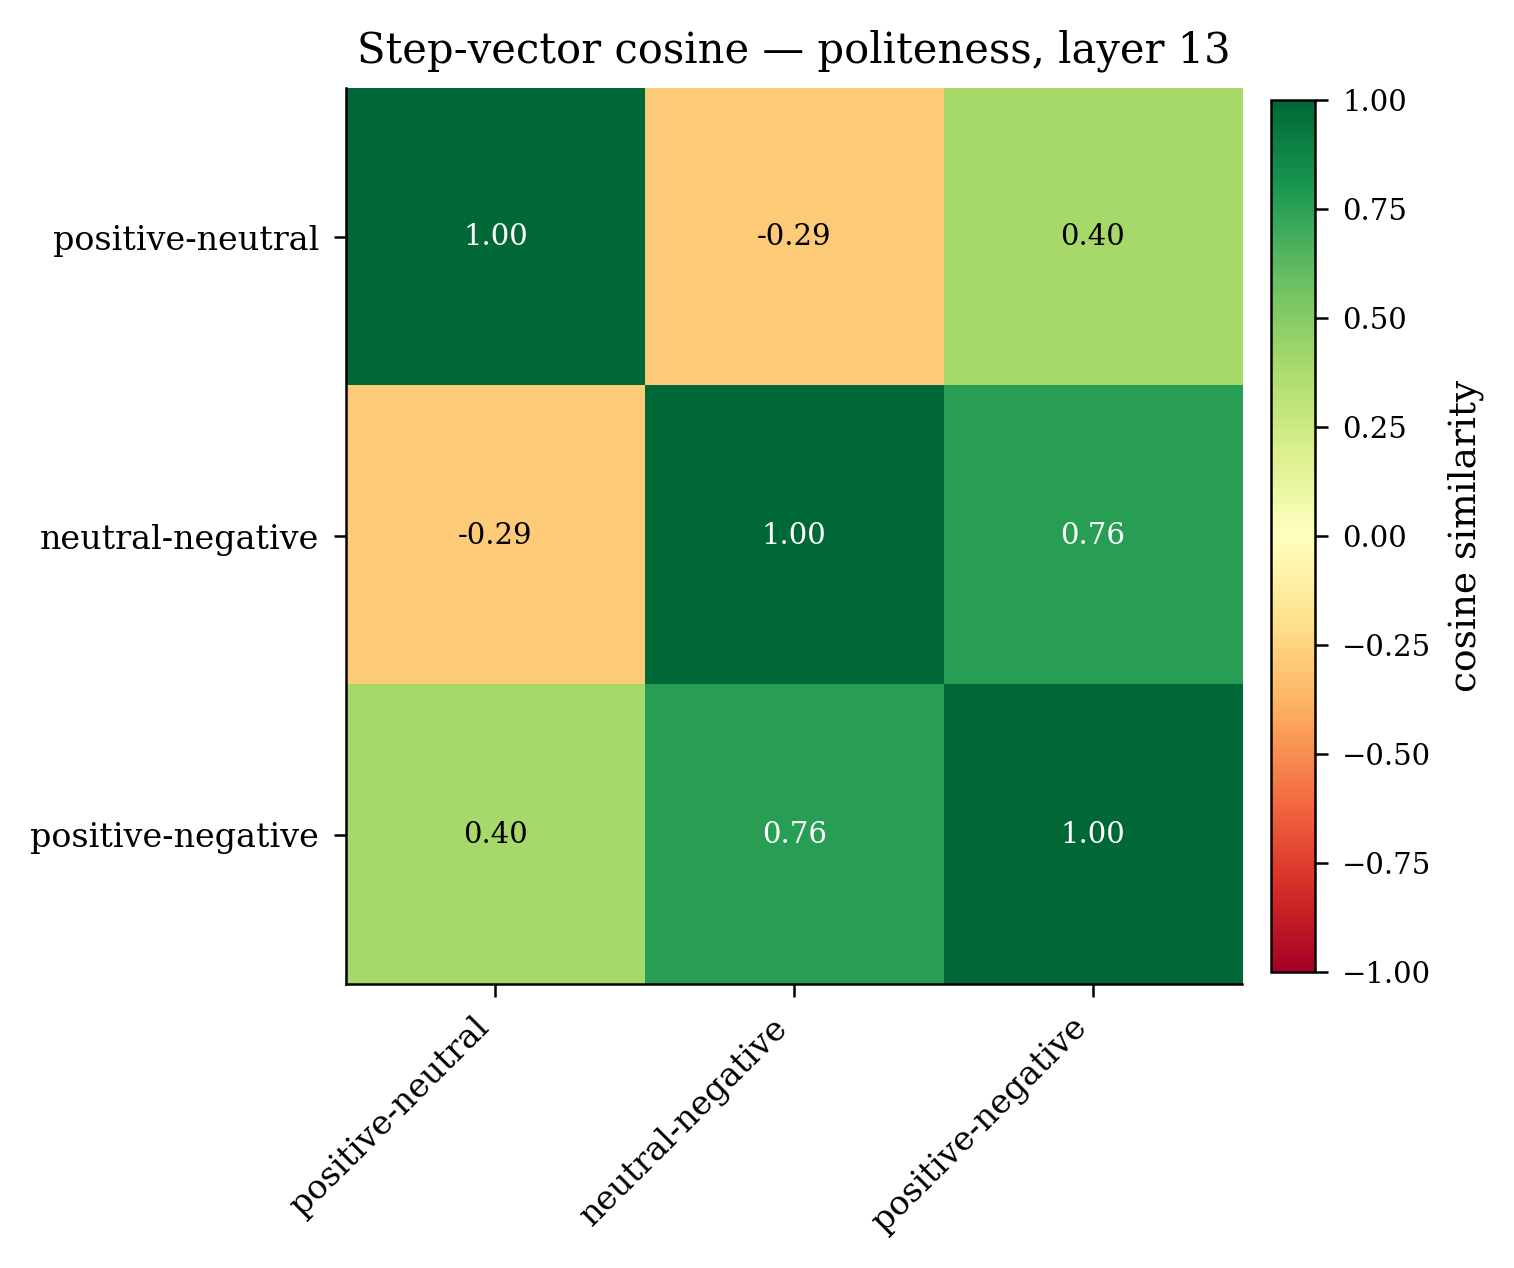
\includegraphics[width=0.49\textwidth]{ordinal_linearity/avg_token/step_vectors_cosine_matrix.png}
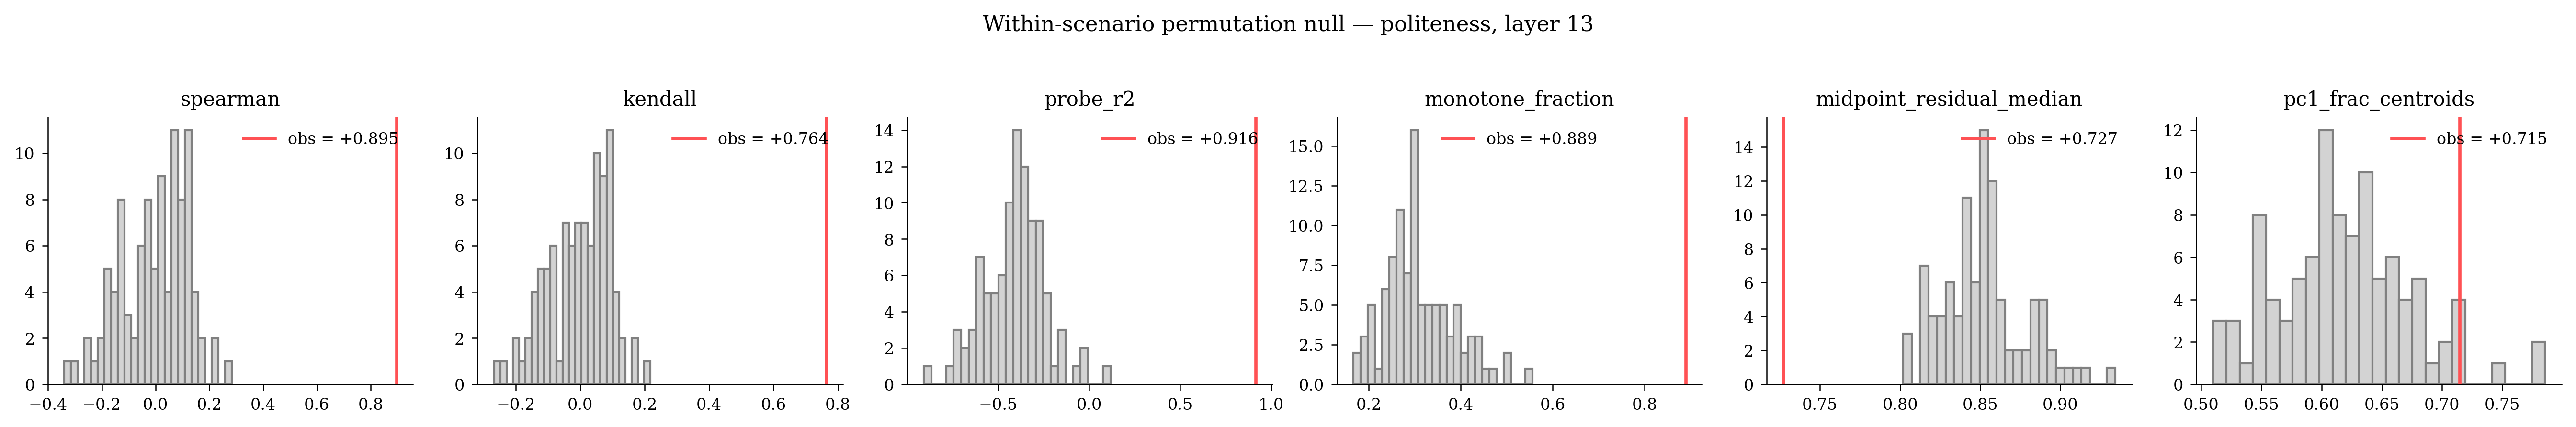
\includegraphics[width=0.49\textwidth]{ordinal_linearity/avg_token/linearity_permutation_null.png}
\caption{Mean pooling; same panels as \Cref{fig:ordinal}.}
\label{fig:ordinal-avg}
\end{figure}

\begin{figure}[t]
\centering

\includegraphics[width=0.49\textwidth]{ordinal_linearity/last_token/inner_products_adjacent_step.png}

\includegraphics[width=0.49\textwidth]{ordinal_linearity/last_token/inner_products_cosine_grid.png}\\[2pt]
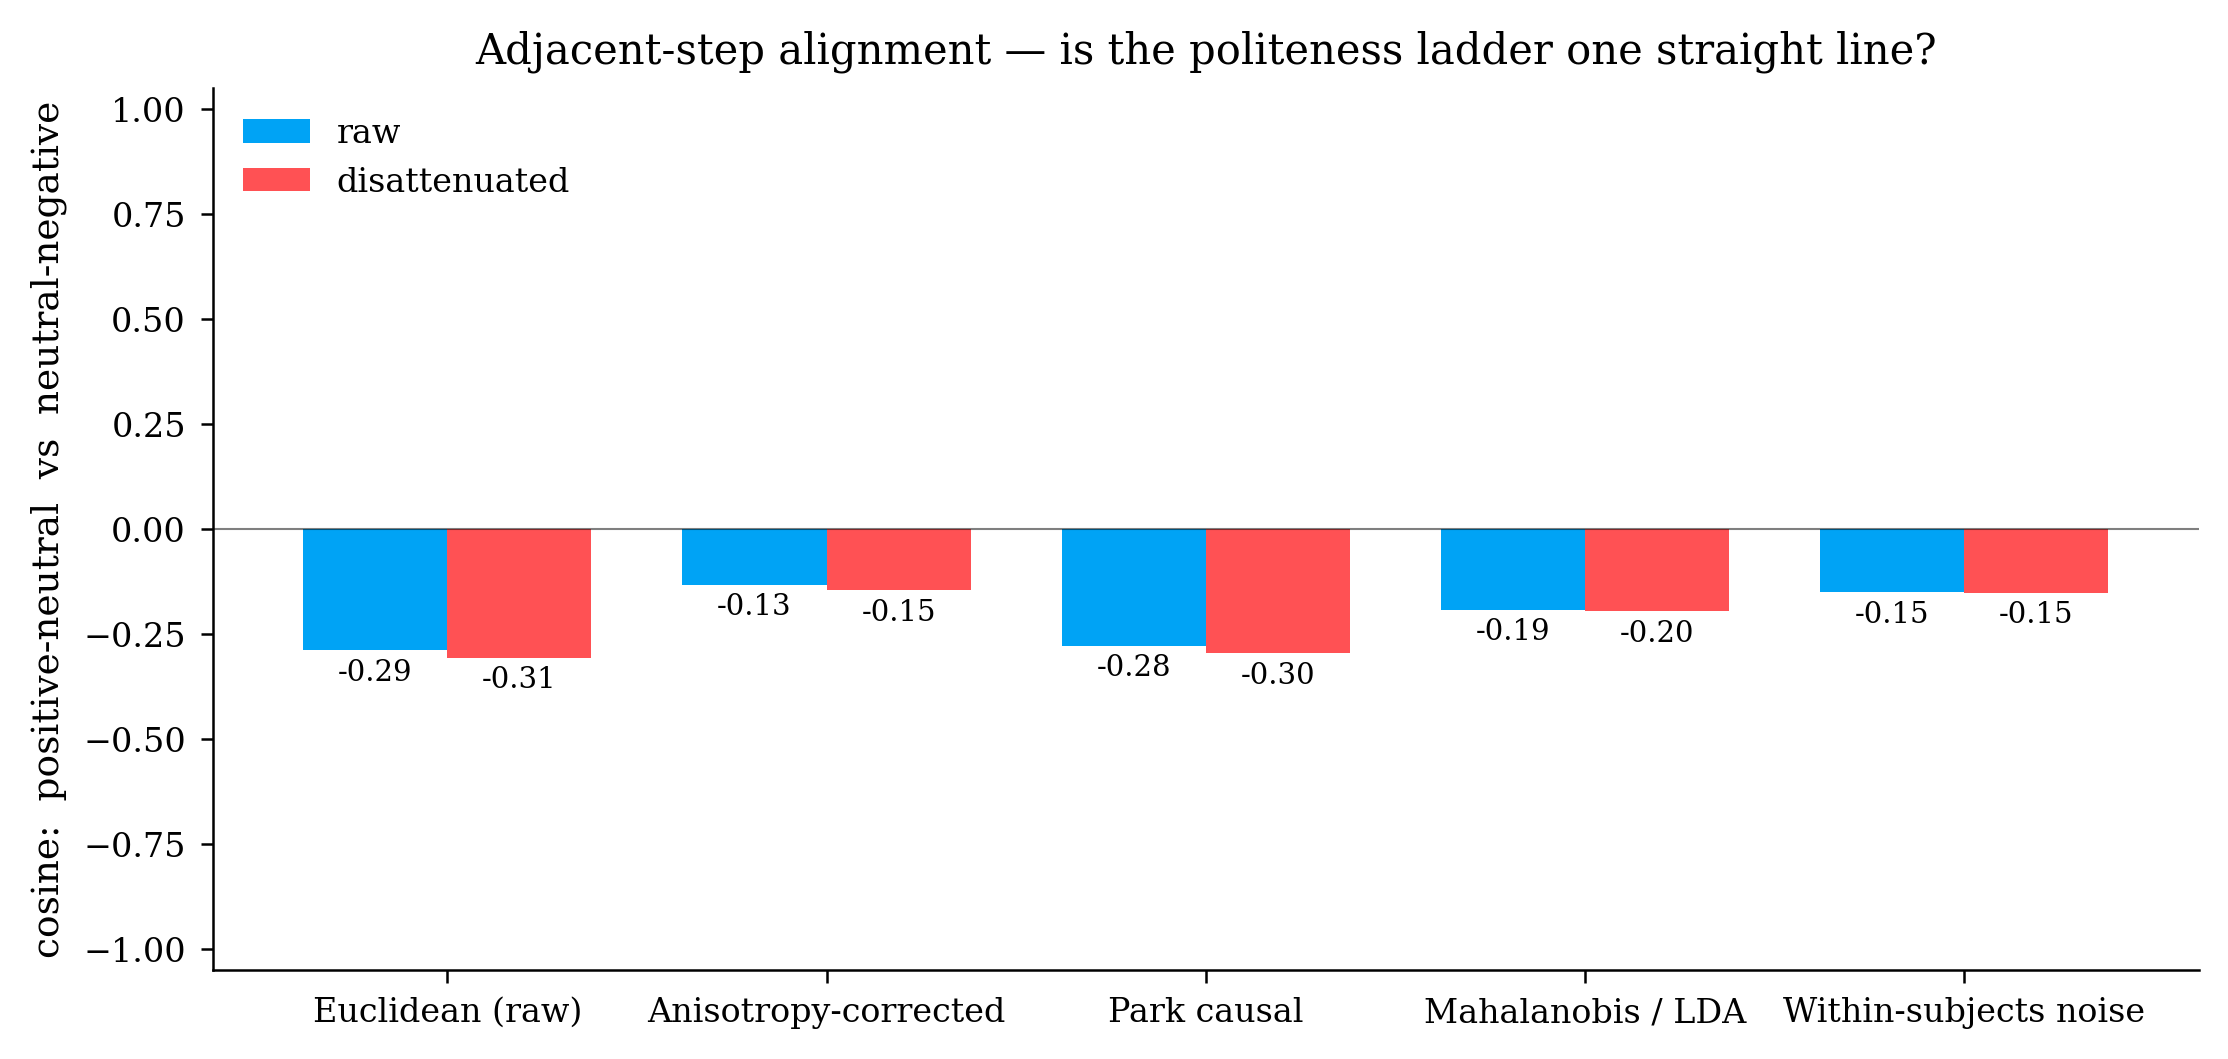
\includegraphics[width=0.49\textwidth]{ordinal_linearity/avg_token/inner_products_adjacent_step.png}
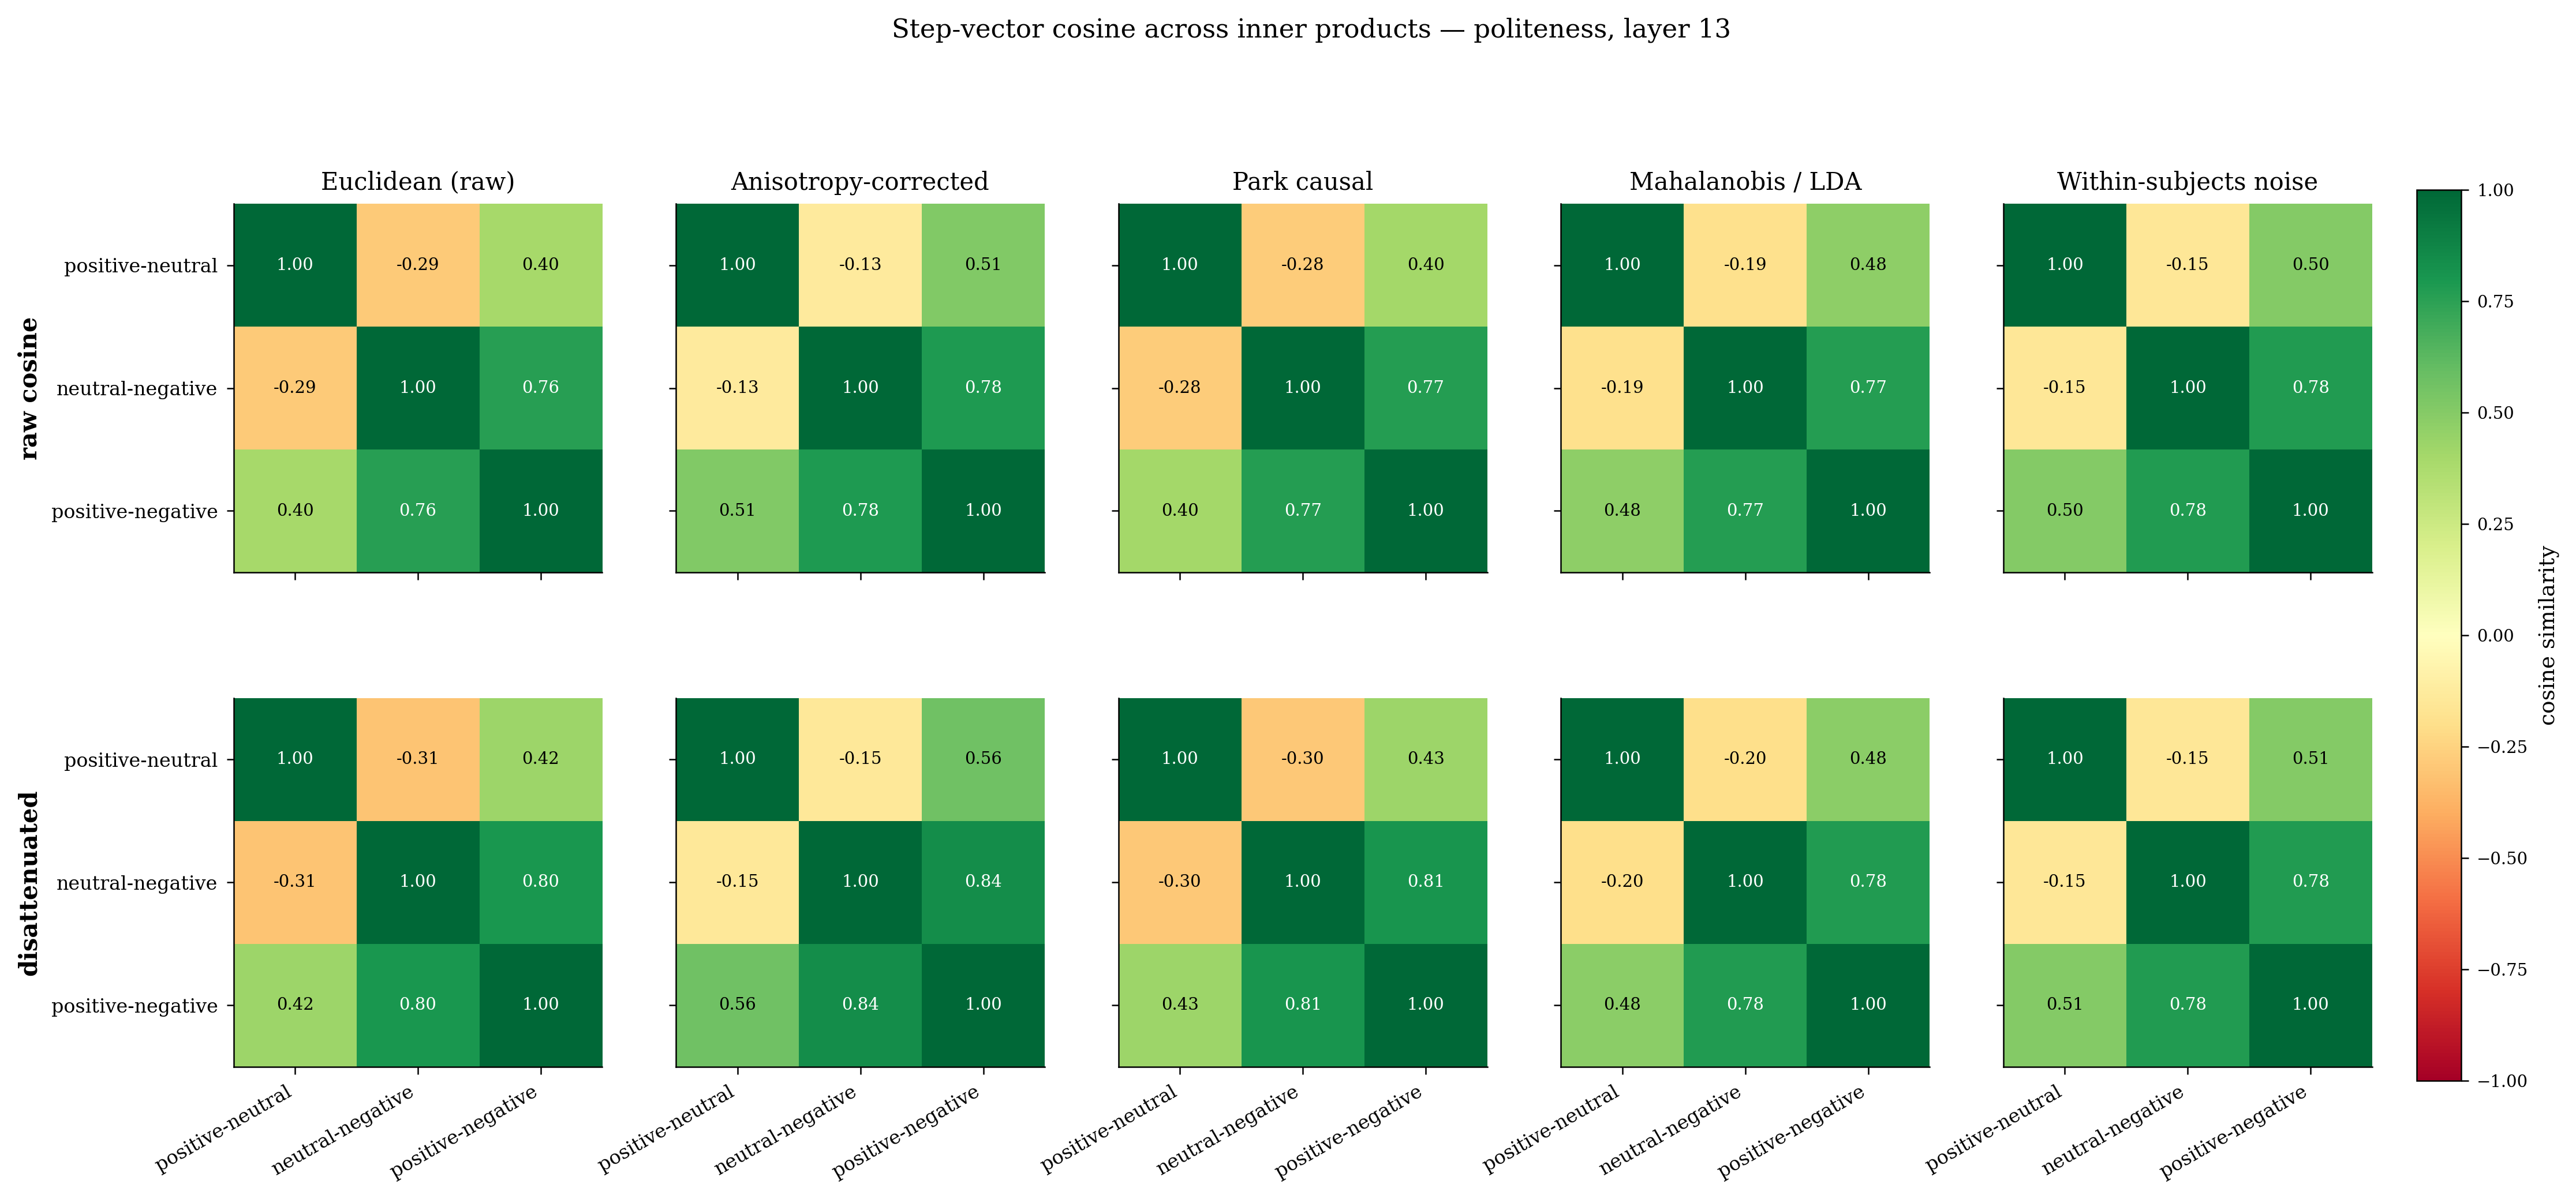
\includegraphics[width=0.49\textwidth]{ordinal_linearity/avg_token/inner_products_cosine_grid.png}
\caption{Inner-product geometry. \emph{Top:} last token. \emph{Bottom:} mean
pooling. \emph{Left:} adjacent-step cosine across the five inner products with
disattenuation. \emph{Right:} the full step-pair cosine grid per inner product.}
\label{fig:inner}
\end{figure}

\begin{figure}[t]
\centering

\includegraphics[width=0.49\textwidth]{ordinal_linearity/last_token/pca_raw_vs_centered.png}

\includegraphics[width=0.49\textwidth]{ordinal_linearity/last_token/per_scenario_grid.png}
\caption{Last token. \emph{Left:} PCA of the level centroids, raw vs.\
within-scenario centered. \emph{Right:} a grid of per-scenario triples showing
the recurring bend.}
\label{fig:pca-last}
\end{figure}

\begin{figure}[t]
\centering
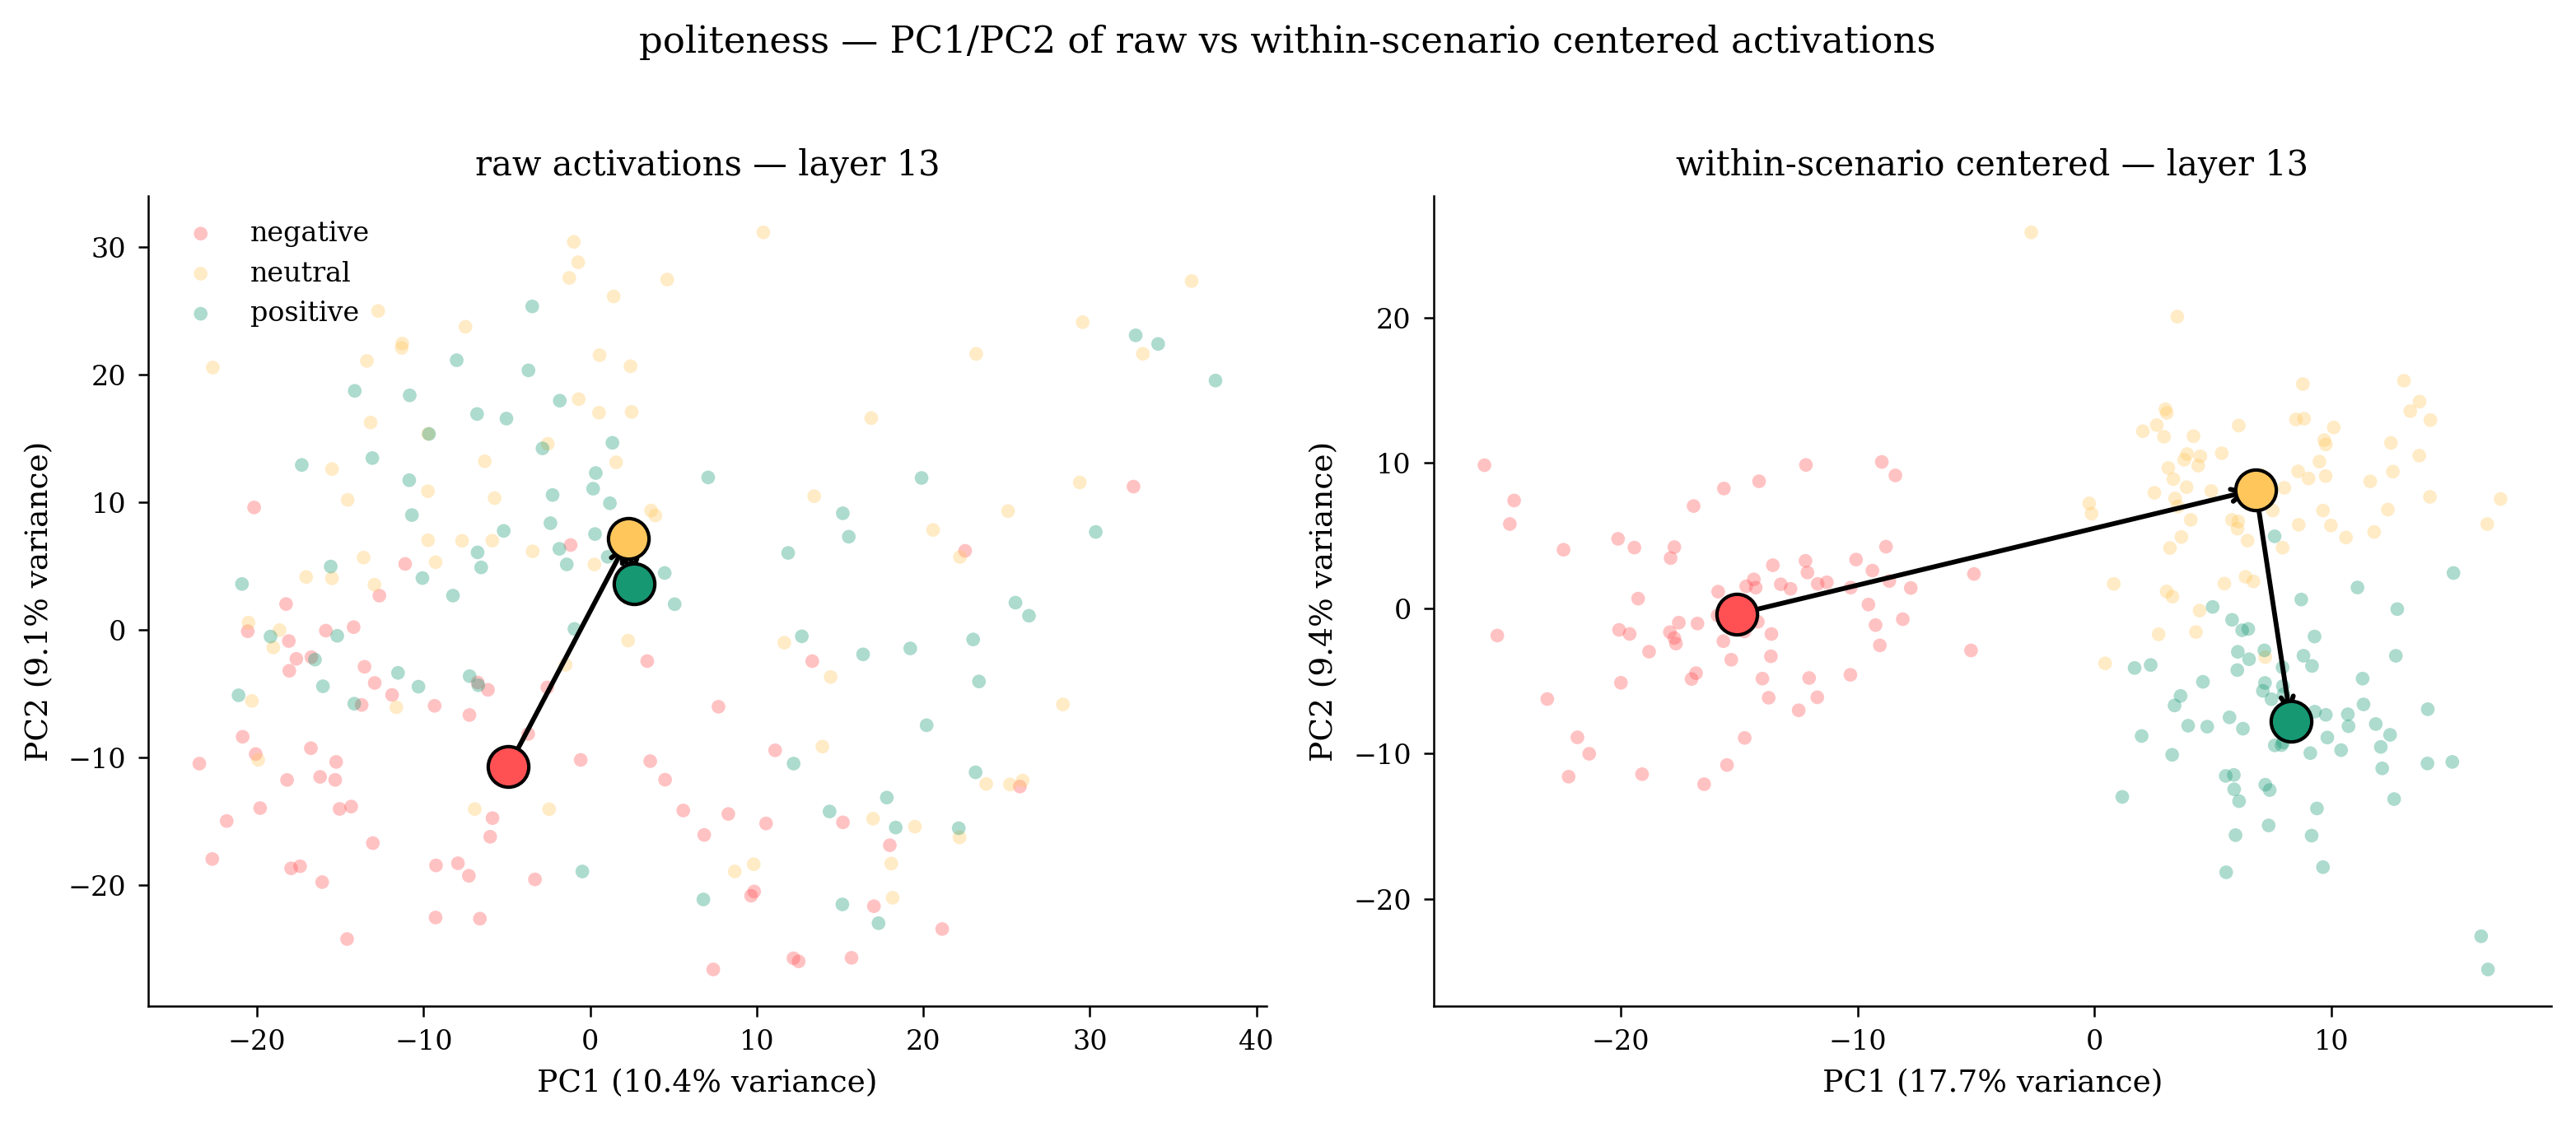
\includegraphics[width=0.49\textwidth]{ordinal_linearity/avg_token/pca_raw_vs_centered.png}
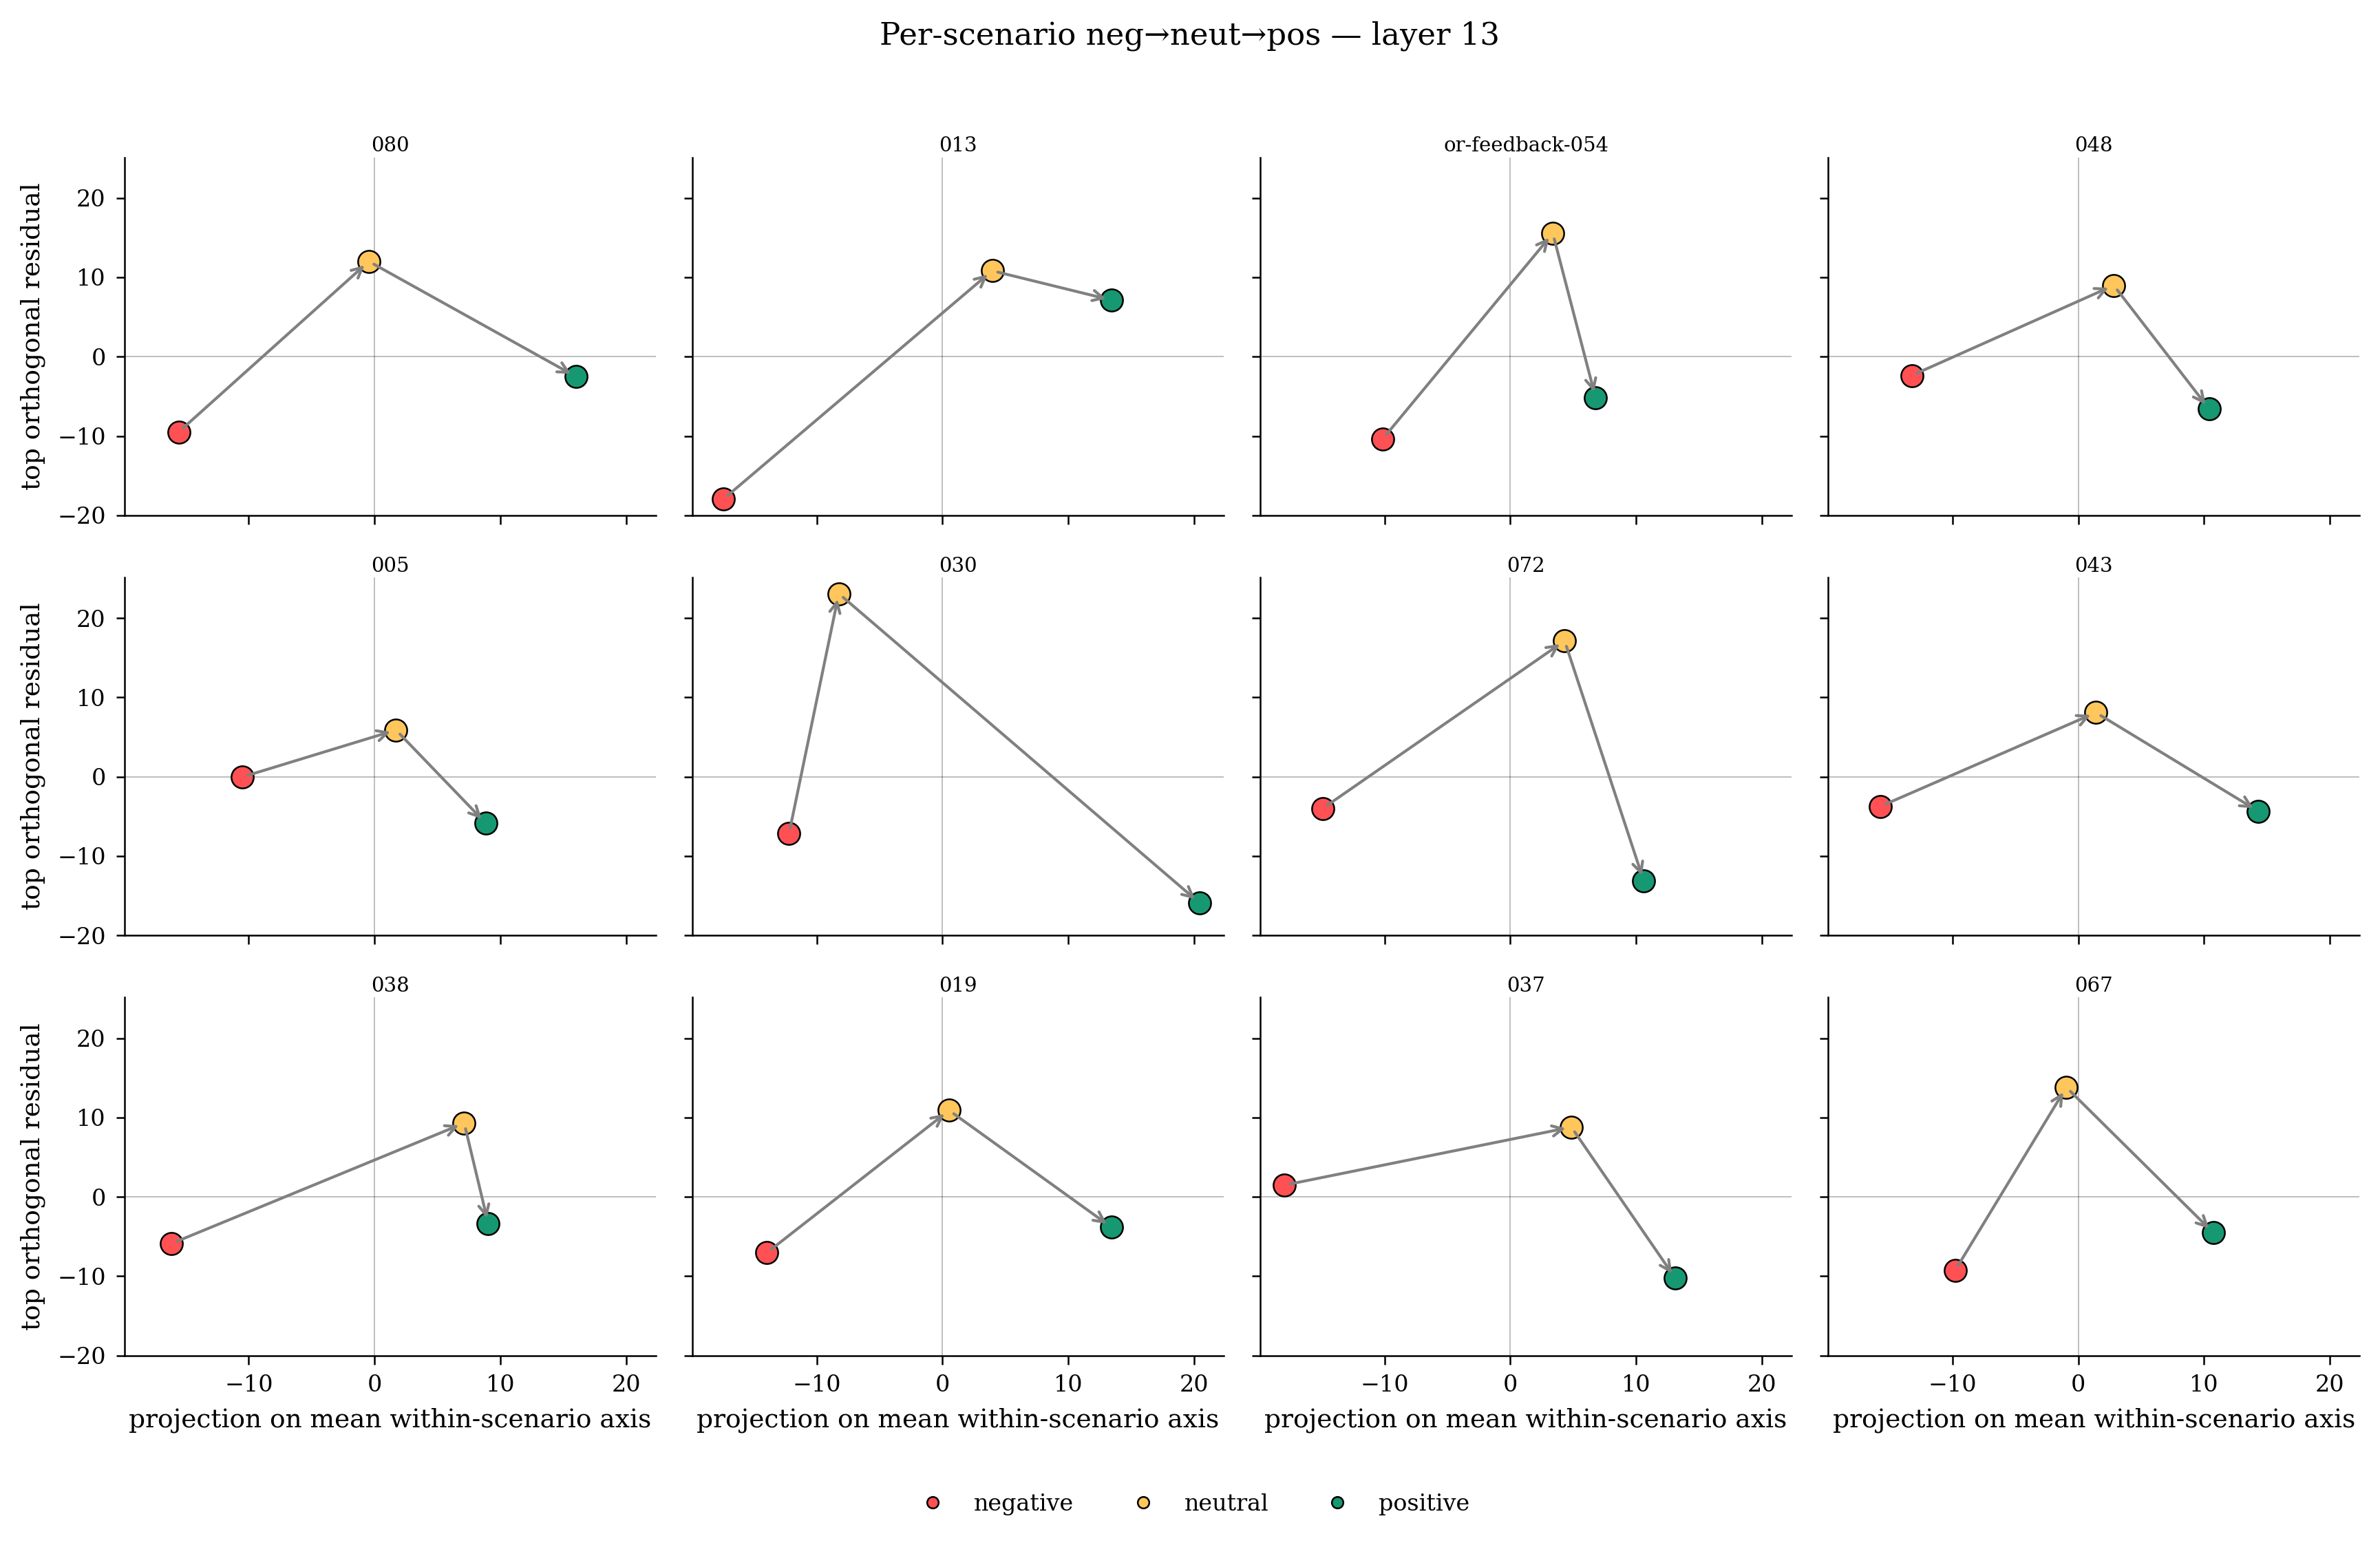
\includegraphics[width=0.49\textwidth]{ordinal_linearity/avg_token/per_scenario_grid.png}
\caption{Mean pooling; same panels as \Cref{fig:pca-last}.}
\label{fig:pca-avg}
\end{figure}

\begin{figure}[t]
\centering

\includegraphics[width=0.49\textwidth]{ordinal_linearity/last_token/linearity_metric_sweep.png}

\includegraphics[width=0.49\textwidth]{ordinal_linearity/last_token/step_vectors_layer_sweep.png}\\[2pt]
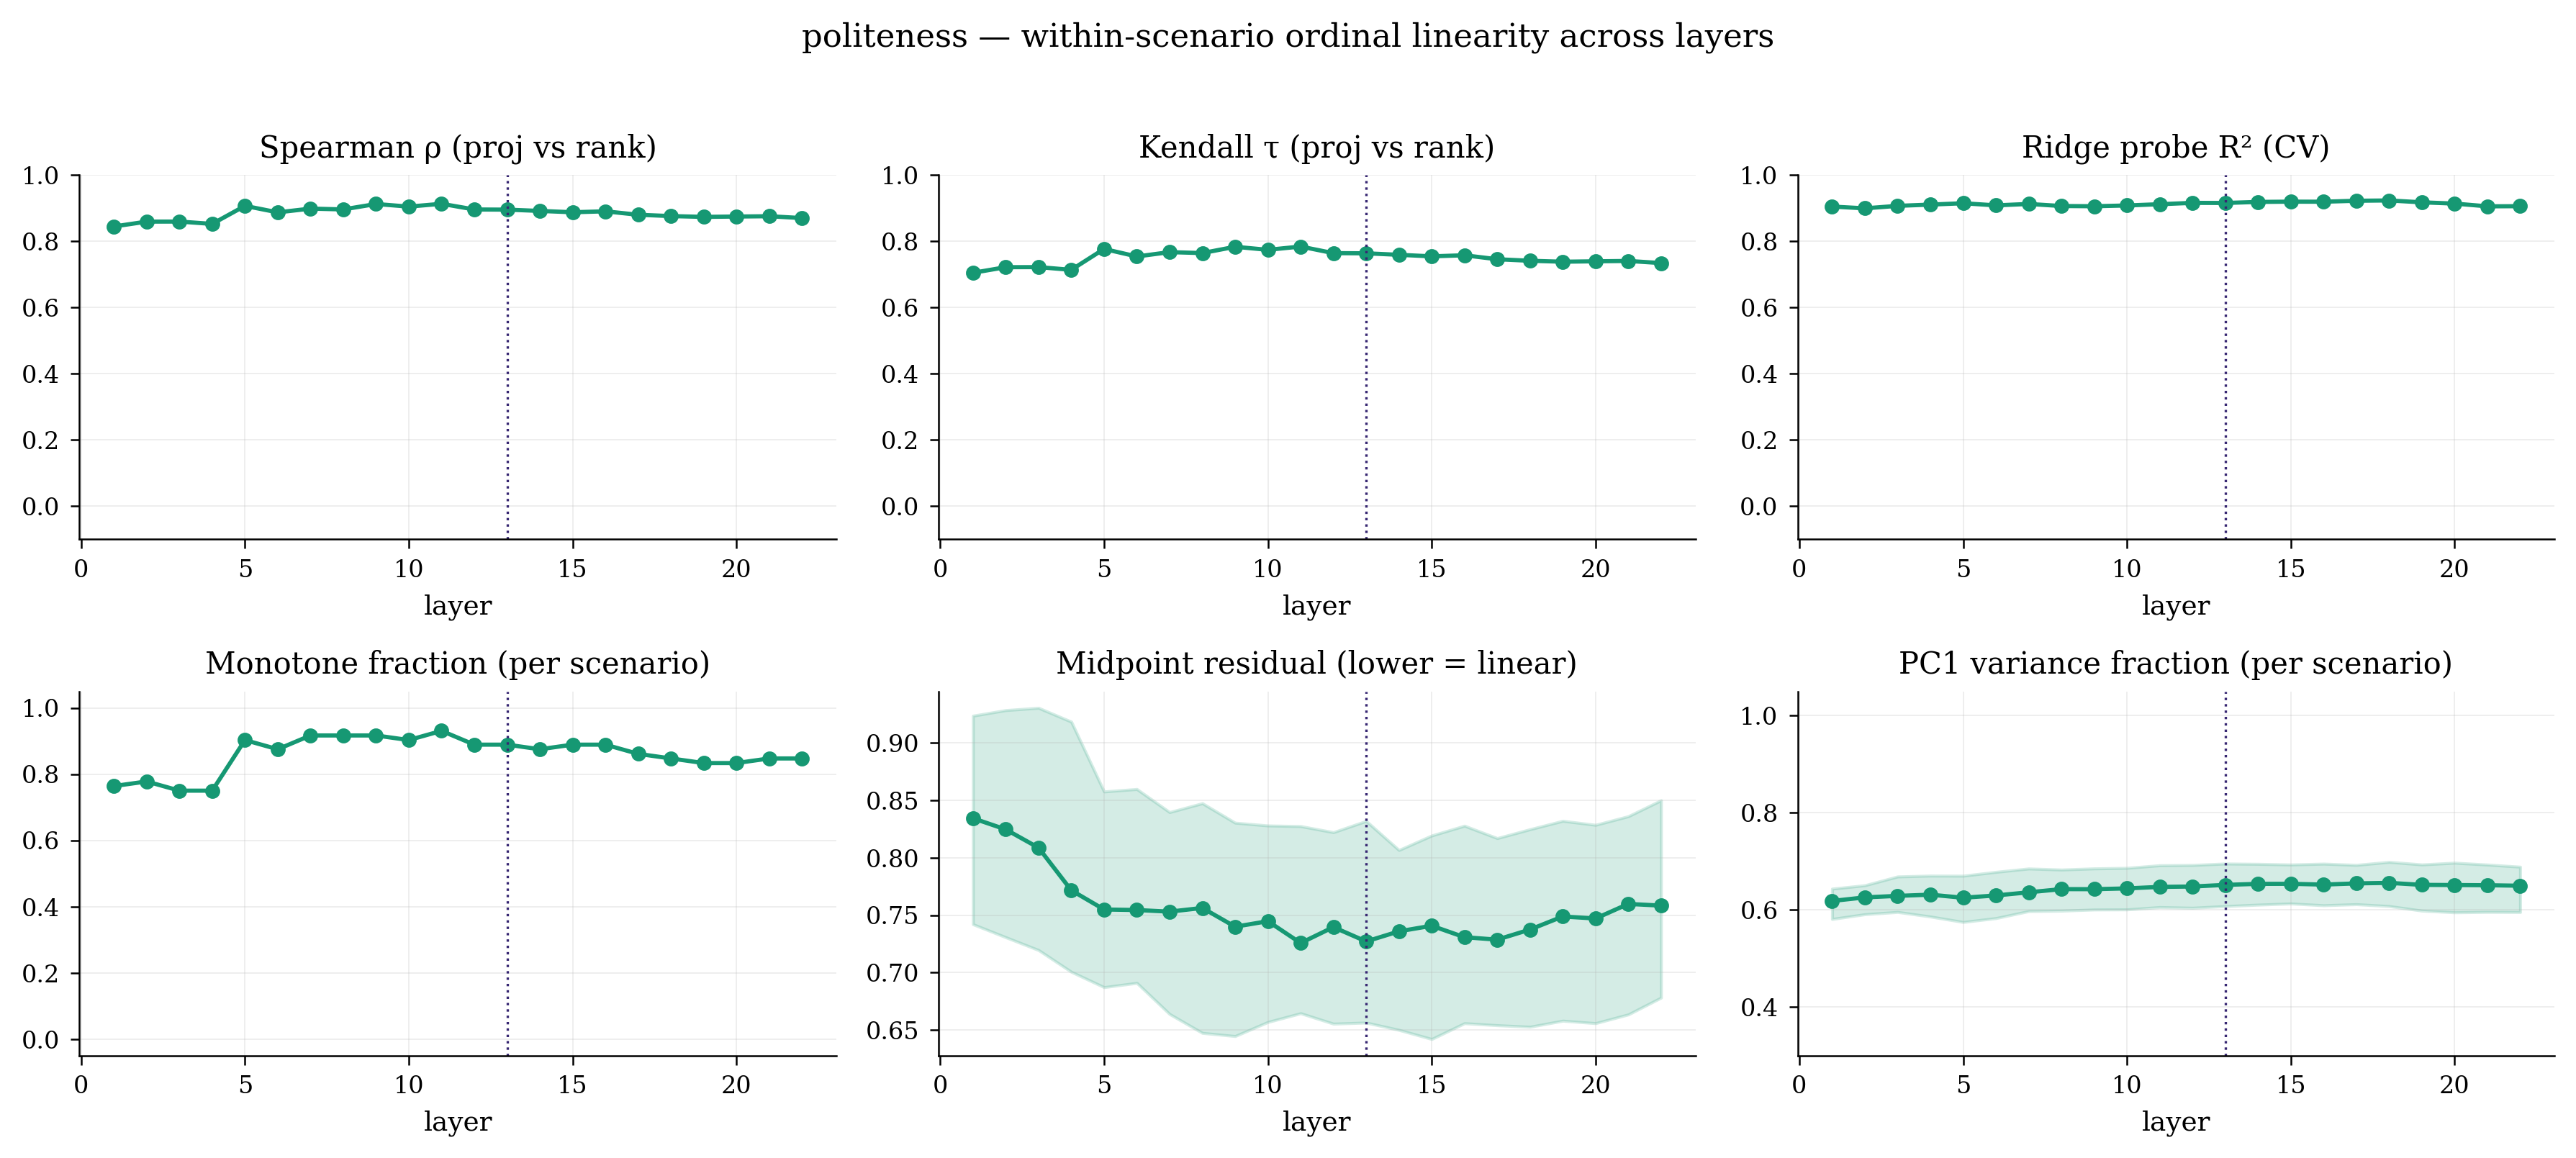
\includegraphics[width=0.49\textwidth]{ordinal_linearity/avg_token/linearity_metric_sweep.png}
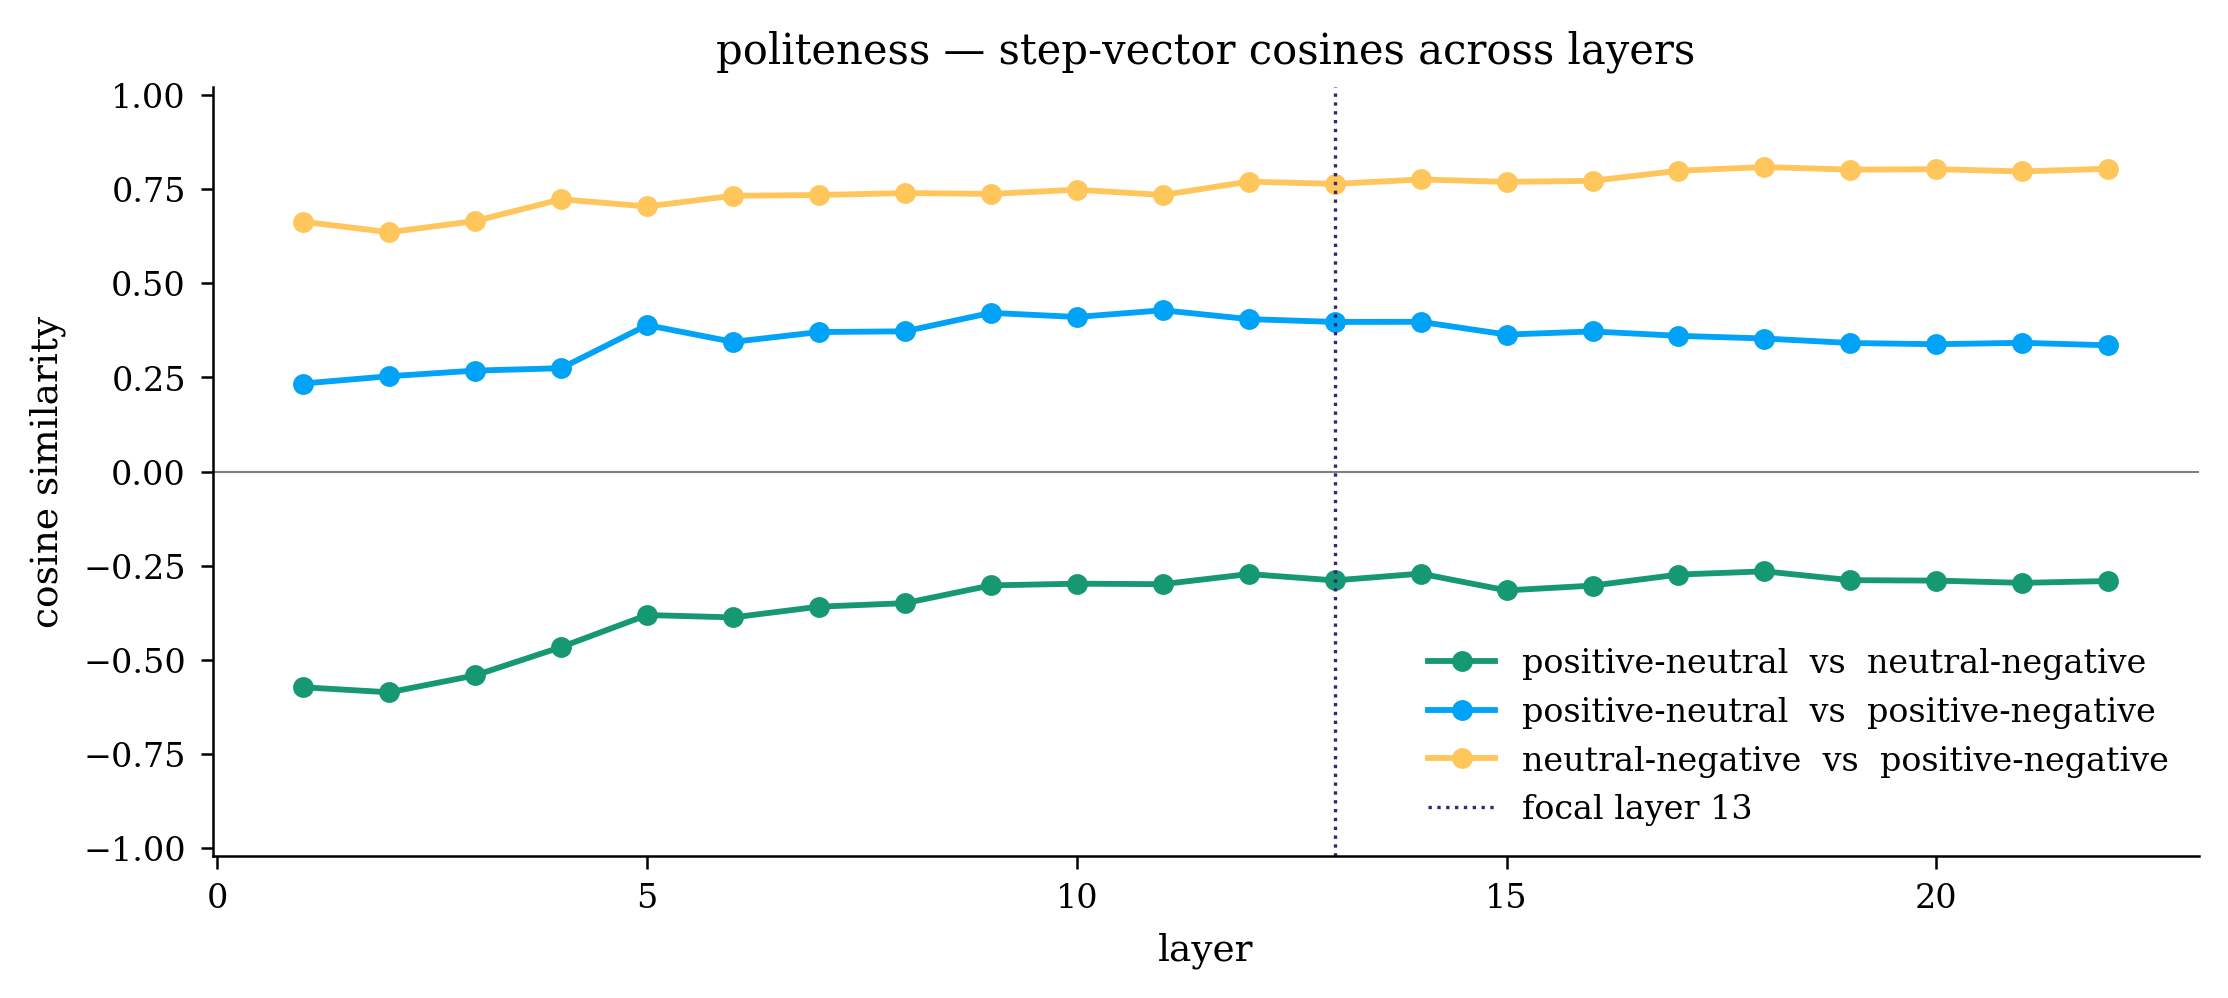
\includegraphics[width=0.49\textwidth]{ordinal_linearity/avg_token/step_vectors_layer_sweep.png}
\caption{Layer robustness. \emph{Top:} last token. \emph{Bottom:} mean pooling.
\emph{Left:} ordinal-linearity metrics across layers. \emph{Right:} step-vector
cosines across layers. The ordering-with-a-bend pattern holds throughout.}
\label{fig:lin-sweep}
\end{figure}

\clearpage
\subsection{Steering geometry and subspace dimensionality}\label{app:res-steering}

\Cref{tab:steer-both} collects the steering decomposition for both poolings.
Throughout, the \emph{valence axis} is the global pole-to-pole politeness
direction (negative$\to$positive), and the \emph{markedness axis} is the shared
off-line direction along which the neutral level is displaced from that line. The
global valence axis is highly reliable ($R=0.94$/$0.96$) but a single vector
captures only $\cos^2=0.20$/$0.25$ of any scenario's own neg$\to$pos contrast.
Adding the markedness axis (the shared plane) raises the captured fraction to
$0.21$/$0.26$, which is $\approx94\%$ of the per-scenario two-dimensional ceiling,
yet the per-scenario planes are themselves spread over many dimensions
(participation ratio $26.5$/$20.0$) and the residual tilt is intent-structured
(within-intent contrast cosine exceeds between-intent by $0.09$/$0.17$). The
supporting figures are \Cref{fig:steering,fig:steering-avg,fig:subspace}.

\begin{table}[t]
\centering
\small
\begin{tabular}{lrr}
\toprule
Quantity & Last token & Mean pooling \\
\midrule
Valence axis reliability $R$ (full)        & 0.938 & 0.956 \\
Mean $\cos$(contrast, global valence)      & 0.428 & 0.493 \\
Steering capture $\cos^2$ (layer 13)       & 0.196 & 0.252 \\
\quad capture IQR                          & [0.127, 0.258] & [0.186, 0.325] \\
Mean $\cos$(bend, markedness axis)         & 0.327 & 0.413 \\
Median principal angle $\theta_1$ ($^\circ$) & 59.3 & 55.3 \\
Median principal angle $\theta_2$ ($^\circ$) & 73.3 & 67.7 \\
Median plane overlap                       & 0.175 & 0.235 \\
Contrast $\cos$ within-intent              & 0.252 & 0.389 \\
Contrast $\cos$ between-intent             & 0.164 & 0.216 \\
\quad within$-$between gap                 & 0.088 & 0.174 \\
Shared plane: valence-1D captured          & 0.139 & 0.167 \\
Shared plane: 2D captured                  & 0.206 & 0.264 \\
Neutral markedness sign consistency        & 95.8\% & 98.6\% \\
Shared-bend $R^2$ (CV)                      & 0.112 & 0.167 \\
Scenarios improved by shared bend          & 83.3\% & 84.7\% \\
Participation ratio                        & 26.5 & 20.0 \\
\bottomrule
\end{tabular}
\caption{Steering and subspace decomposition, layer~13. A reproducible global
axis coexists with low per-scenario capture, an intent-structured residual tilt,
and a high-dimensional spread of per-scenario planes---no single universal
steering direction.}
\label{tab:steer-both}
\end{table}

\begin{figure}[t]
\centering

\includegraphics[width=0.32\textwidth]{trait_geometry/last_token/steering_direction.png}

\includegraphics[width=0.32\textwidth]{ordinal_linearity/last_token/steering_axis_sweep.png}

\includegraphics[width=0.32\textwidth]{trait_geometry/last_token/shared_plane.png}
\caption{No universal steering direction (last token). \emph{Left:} per-scenario
alignment to the global axis and plane-tilt angles. \emph{Middle:} steering
capture ($\cos^2$) across layers, plateauing near $0.20$. \emph{Right:} the
shared (valence,~markedness) plane.}
\label{fig:steering}
\end{figure}

\begin{figure}[t]
\centering
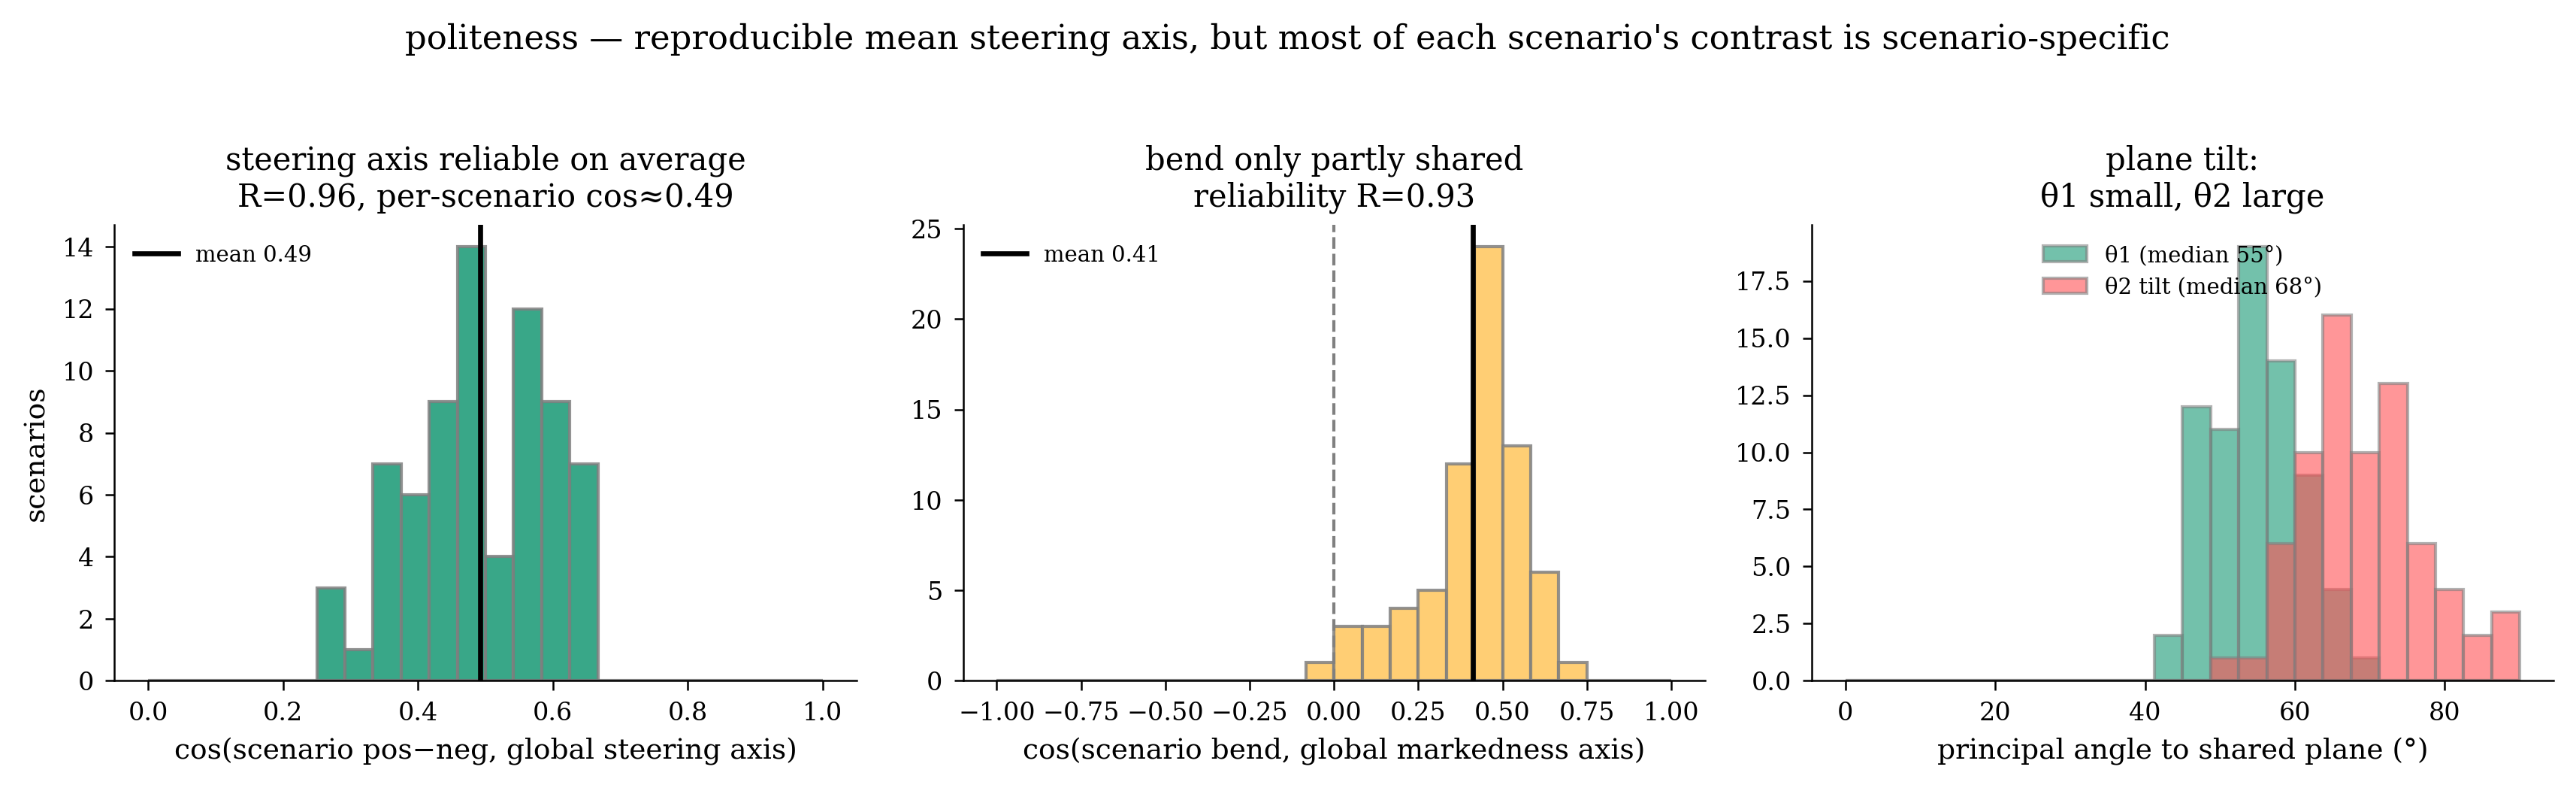
\includegraphics[width=0.32\textwidth]{trait_geometry/avg_token/steering_direction.png}
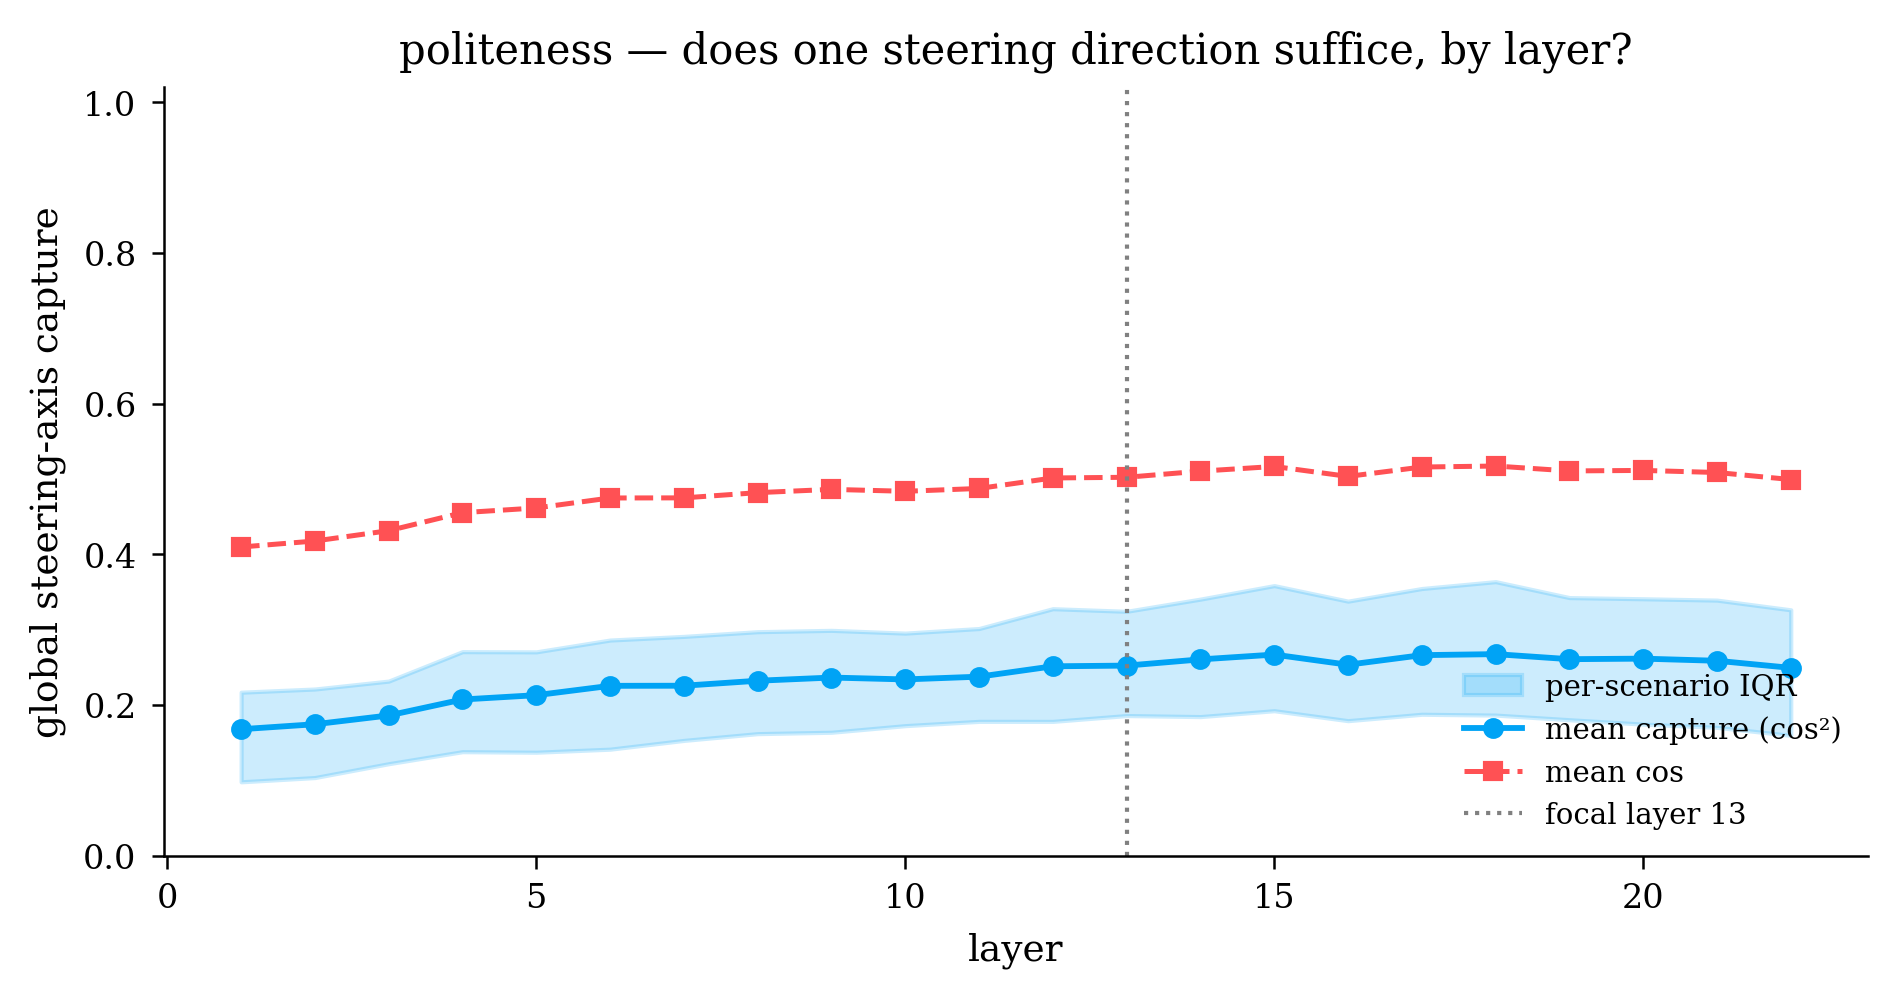
\includegraphics[width=0.32\textwidth]{ordinal_linearity/avg_token/steering_axis_sweep.png}
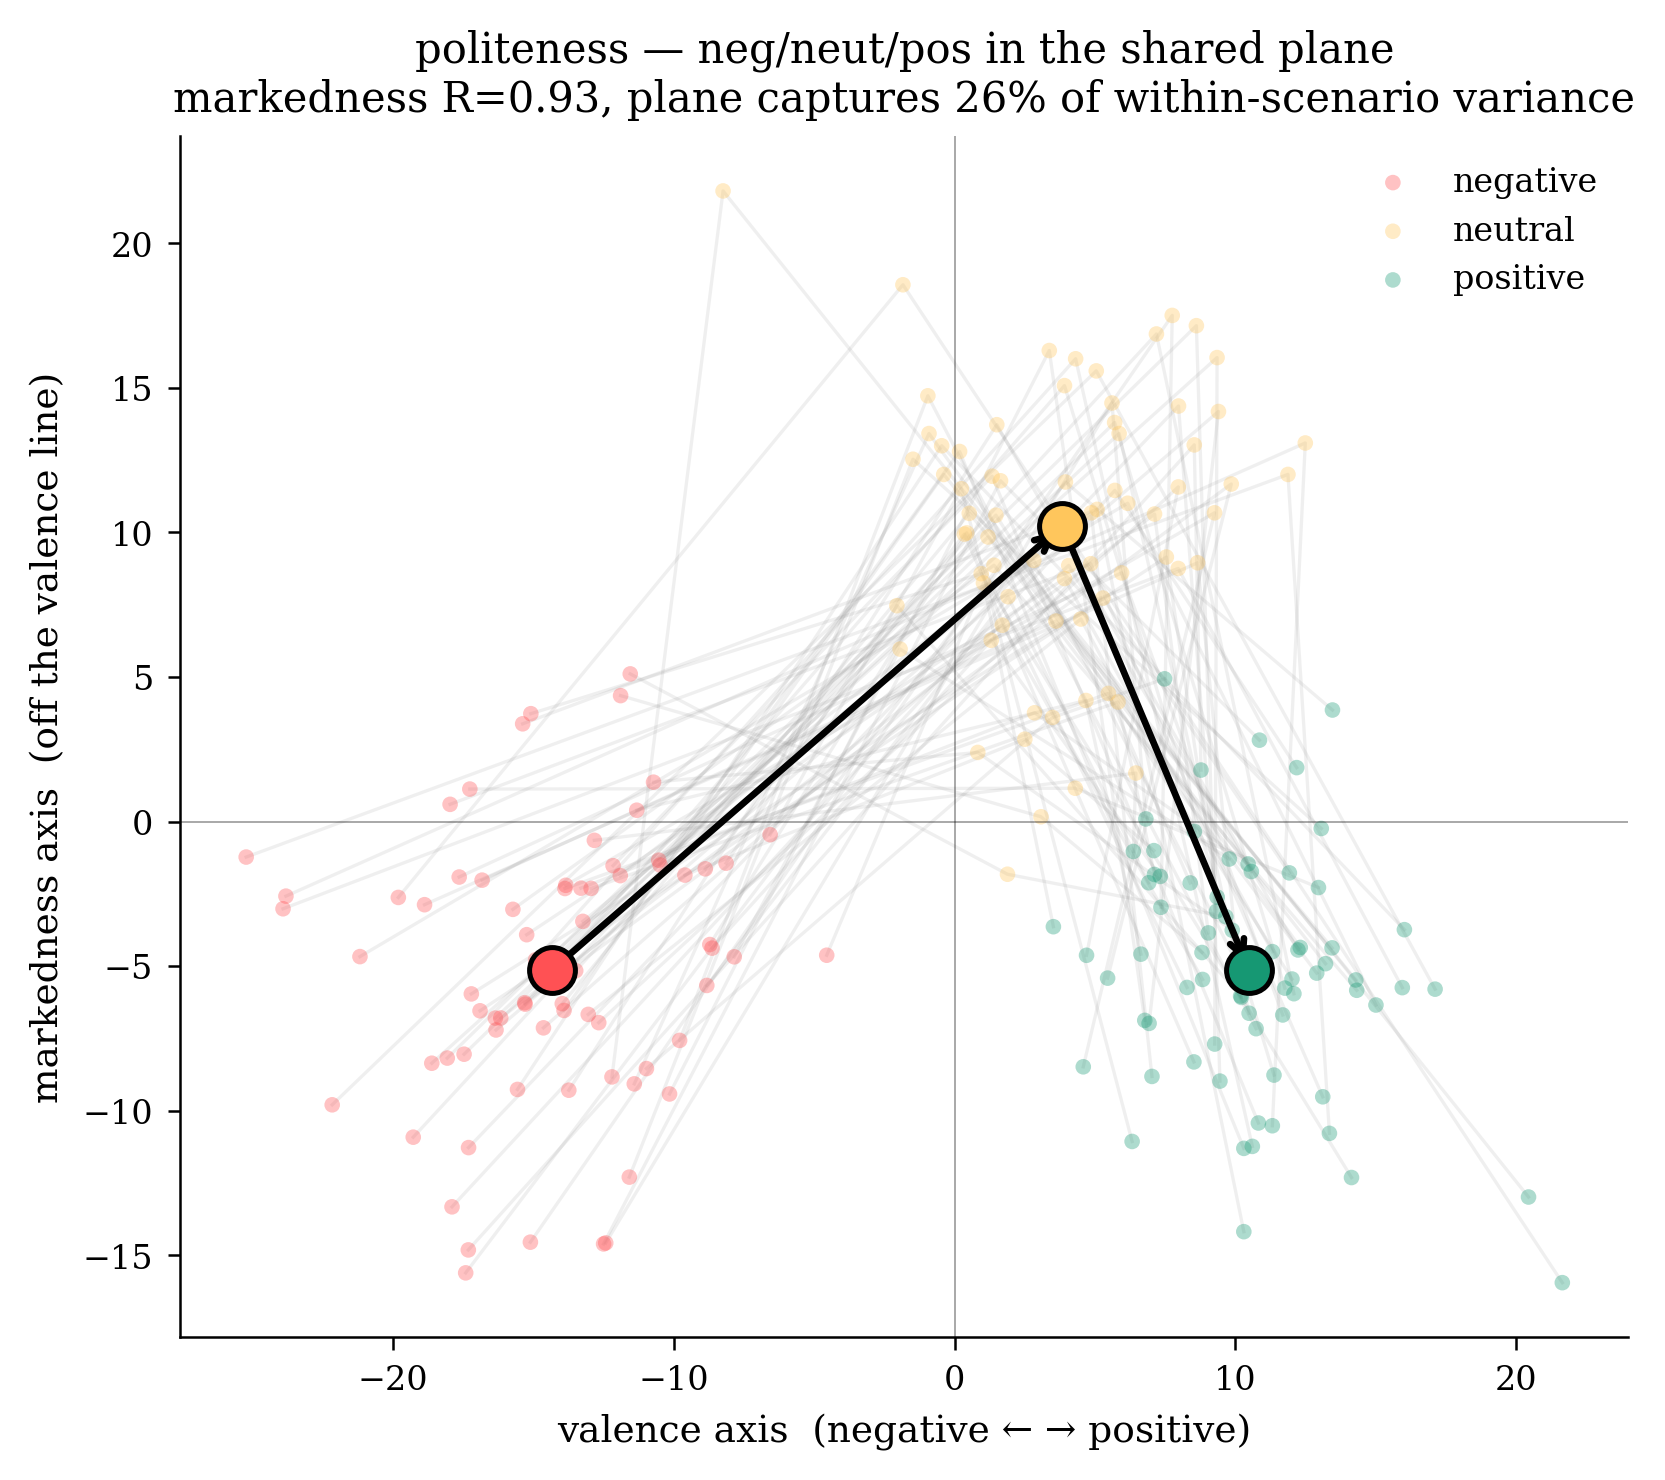
\includegraphics[width=0.32\textwidth]{trait_geometry/avg_token/shared_plane.png}
\caption{No universal steering direction (mean pooling); same panels as
\Cref{fig:steering}. Capture plateaus near $0.25$.}
\label{fig:steering-avg}
\end{figure}

\begin{figure}[t]
\centering

\includegraphics[width=0.49\textwidth]{trait_geometry/last_token/subspace_spectrum.png}
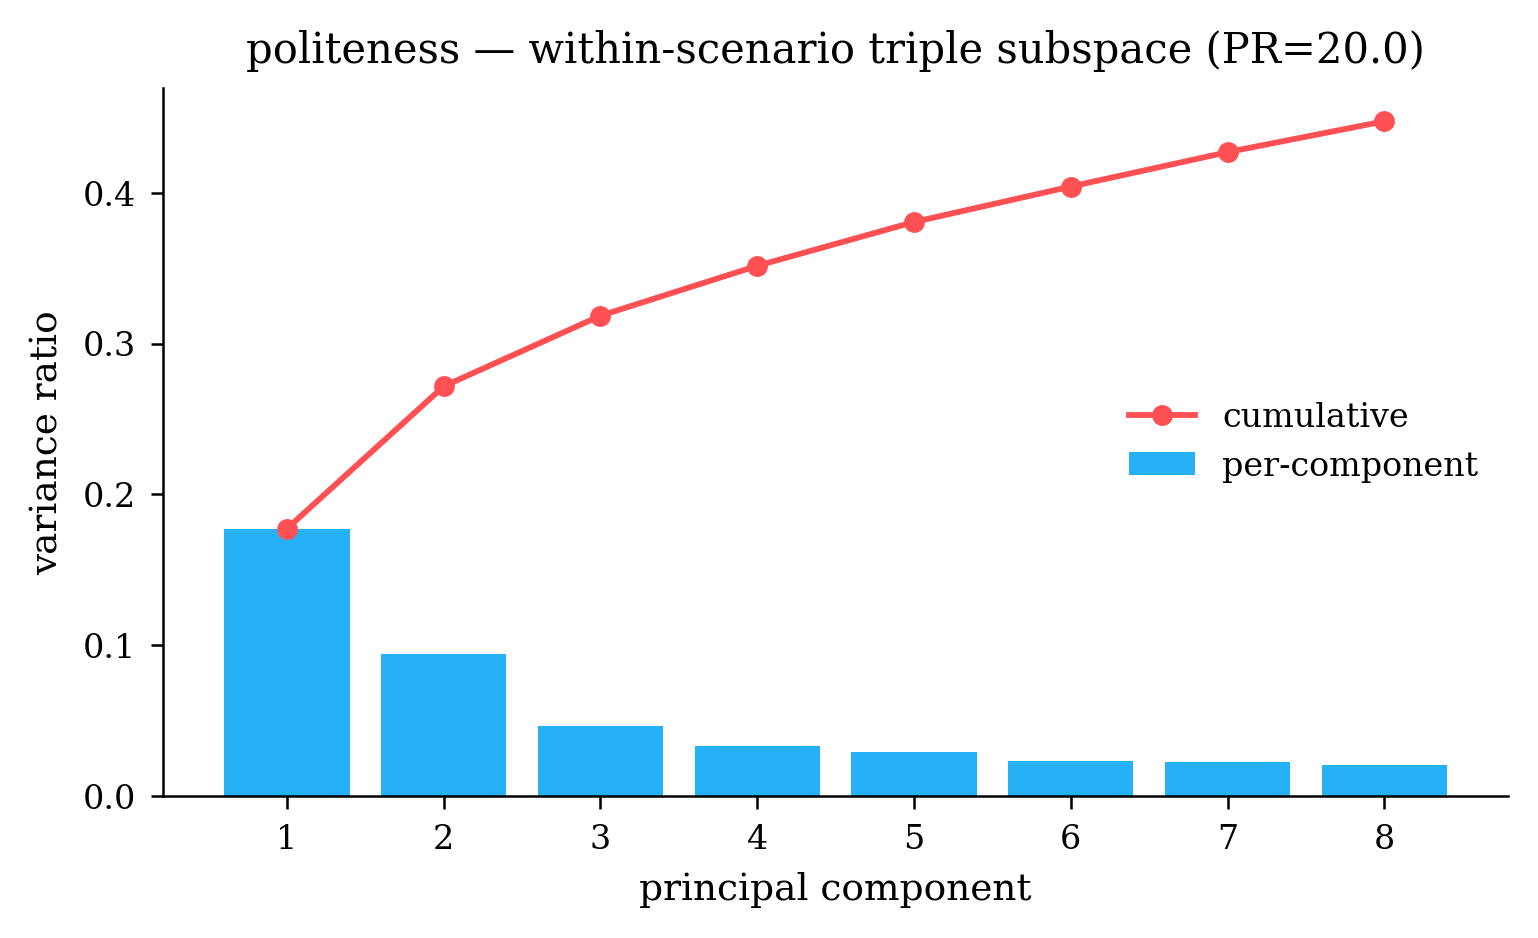
\includegraphics[width=0.49\textwidth]{trait_geometry/avg_token/subspace_spectrum.png}
\caption{Subspace spectrum of the per-scenario centred triples. \emph{Left:} last
token (participation ratio $26.5$). \emph{Right:} mean pooling ($20.0$). The
politeness variation is spread across many dimensions, not confined to a
low-rank shared subspace.}
\label{fig:subspace}
\end{figure}

\end{document}